% Options for packages loaded elsewhere
\PassOptionsToPackage{unicode}{hyperref}
\PassOptionsToPackage{hyphens}{url}
\documentclass[
]{article}
\usepackage{xcolor}
\usepackage{amsmath,amssymb}
\setcounter{secnumdepth}{5}
\usepackage{iftex}
\ifPDFTeX
  \usepackage[T1]{fontenc}
  \usepackage[utf8]{inputenc}
  \usepackage{textcomp} % provide euro and other symbols
\else % if luatex or xetex
  \usepackage{unicode-math} % this also loads fontspec
  \defaultfontfeatures{Scale=MatchLowercase}
  \defaultfontfeatures[\rmfamily]{Ligatures=TeX,Scale=1}
\fi
\usepackage{lmodern}
\ifPDFTeX\else
  % xetex/luatex font selection
\fi
% Use upquote if available, for straight quotes in verbatim environments
\IfFileExists{upquote.sty}{\usepackage{upquote}}{}
\IfFileExists{microtype.sty}{% use microtype if available
  \usepackage[]{microtype}
  \UseMicrotypeSet[protrusion]{basicmath} % disable protrusion for tt fonts
}{}
\makeatletter
\@ifundefined{KOMAClassName}{% if non-KOMA class
  \IfFileExists{parskip.sty}{%
    \usepackage{parskip}
  }{% else
    \setlength{\parindent}{0pt}
    \setlength{\parskip}{6pt plus 2pt minus 1pt}}
}{% if KOMA class
  \KOMAoptions{parskip=half}}
\makeatother
\usepackage{color}
\usepackage{fancyvrb}
\newcommand{\VerbBar}{|}
\newcommand{\VERB}{\Verb[commandchars=\\\{\}]}
\DefineVerbatimEnvironment{Highlighting}{Verbatim}{commandchars=\\\{\}}
% Add ',fontsize=\small' for more characters per line
\newenvironment{Shaded}{}{}
\newcommand{\AlertTok}[1]{\textcolor[rgb]{1.00,0.00,0.00}{\textbf{#1}}}
\newcommand{\AnnotationTok}[1]{\textcolor[rgb]{0.38,0.63,0.69}{\textbf{\textit{#1}}}}
\newcommand{\AttributeTok}[1]{\textcolor[rgb]{0.49,0.56,0.16}{#1}}
\newcommand{\BaseNTok}[1]{\textcolor[rgb]{0.25,0.63,0.44}{#1}}
\newcommand{\BuiltInTok}[1]{\textcolor[rgb]{0.00,0.50,0.00}{#1}}
\newcommand{\CharTok}[1]{\textcolor[rgb]{0.25,0.44,0.63}{#1}}
\newcommand{\CommentTok}[1]{\textcolor[rgb]{0.38,0.63,0.69}{\textit{#1}}}
\newcommand{\CommentVarTok}[1]{\textcolor[rgb]{0.38,0.63,0.69}{\textbf{\textit{#1}}}}
\newcommand{\ConstantTok}[1]{\textcolor[rgb]{0.53,0.00,0.00}{#1}}
\newcommand{\ControlFlowTok}[1]{\textcolor[rgb]{0.00,0.44,0.13}{\textbf{#1}}}
\newcommand{\DataTypeTok}[1]{\textcolor[rgb]{0.56,0.13,0.00}{#1}}
\newcommand{\DecValTok}[1]{\textcolor[rgb]{0.25,0.63,0.44}{#1}}
\newcommand{\DocumentationTok}[1]{\textcolor[rgb]{0.73,0.13,0.13}{\textit{#1}}}
\newcommand{\ErrorTok}[1]{\textcolor[rgb]{1.00,0.00,0.00}{\textbf{#1}}}
\newcommand{\ExtensionTok}[1]{#1}
\newcommand{\FloatTok}[1]{\textcolor[rgb]{0.25,0.63,0.44}{#1}}
\newcommand{\FunctionTok}[1]{\textcolor[rgb]{0.02,0.16,0.49}{#1}}
\newcommand{\ImportTok}[1]{\textcolor[rgb]{0.00,0.50,0.00}{\textbf{#1}}}
\newcommand{\InformationTok}[1]{\textcolor[rgb]{0.38,0.63,0.69}{\textbf{\textit{#1}}}}
\newcommand{\KeywordTok}[1]{\textcolor[rgb]{0.00,0.44,0.13}{\textbf{#1}}}
\newcommand{\NormalTok}[1]{#1}
\newcommand{\OperatorTok}[1]{\textcolor[rgb]{0.40,0.40,0.40}{#1}}
\newcommand{\OtherTok}[1]{\textcolor[rgb]{0.00,0.44,0.13}{#1}}
\newcommand{\PreprocessorTok}[1]{\textcolor[rgb]{0.74,0.48,0.00}{#1}}
\newcommand{\RegionMarkerTok}[1]{#1}
\newcommand{\SpecialCharTok}[1]{\textcolor[rgb]{0.25,0.44,0.63}{#1}}
\newcommand{\SpecialStringTok}[1]{\textcolor[rgb]{0.73,0.40,0.53}{#1}}
\newcommand{\StringTok}[1]{\textcolor[rgb]{0.25,0.44,0.63}{#1}}
\newcommand{\VariableTok}[1]{\textcolor[rgb]{0.10,0.09,0.49}{#1}}
\newcommand{\VerbatimStringTok}[1]{\textcolor[rgb]{0.25,0.44,0.63}{#1}}
\newcommand{\WarningTok}[1]{\textcolor[rgb]{0.38,0.63,0.69}{\textbf{\textit{#1}}}}
\usepackage{longtable,booktabs,array}
\usepackage{calc} % for calculating minipage widths
\usepackage{graphicx} % v2.8 — needed for figures/fig5_v28_recalibration
% Correct order of tables after \paragraph or \subparagraph
\usepackage{etoolbox}
\makeatletter
\patchcmd\longtable{\par}{\if@noskipsec\mbox{}\fi\par}{}{}
\makeatother
% Allow footnotes in longtable head/foot
\IfFileExists{footnotehyper.sty}{\usepackage{footnotehyper}}{\usepackage{footnote}}
\makesavenoteenv{longtable}
\setlength{\emergencystretch}{3em} % prevent overfull lines
\providecommand{\tightlist}{%
  \setlength{\itemsep}{0pt}\setlength{\parskip}{0pt}}
\usepackage{bookmark}
\IfFileExists{xurl.sty}{\usepackage{xurl}}{} % add URL line breaks if available
\urlstyle{same}
\hypersetup{
  hidelinks,
  pdfcreator={LaTeX via pandoc}}

\author{Alberto Giovanni Gerli\\
Tourbillon Tech Srl, Padova, Italy\\
Università degli Studi di Milano, Italy\\
\texttt{alberto@albertogerli.it}}
\date{Version 2.8 --- May 2026}

\begin{document}

\section{A Calibrated LLM-Conditioned Agent-Based Model of Public
Opinion Dynamics with Null-Baseline Benchmarking, Data-Contamination
Auditing, and Online
Assimilation}\label{a-calibrated-llm-conditioned-agent-based-model-of-public-opinion-dynamics-with-null-baseline-benchmarking-data-contamination-auditing-and-online-assimilation}

\textbf{Alberto Giovanni Gerli}\^{}\{1,2\}

\^{}1 Tourbillon Tech Srl, Padova, Italy \^{}2 Dipartimento di Scienze
Cliniche e di Comunità, Università degli Studi di Milano, Italy

\textbf{Keywords:} opinion dynamics, agent-based modeling, large
language models, Bayesian calibration, Ensemble Kalman filter,
computational social science, Diebold--Mariano test, null baselines,
data contamination, blinding protocol

\begin{center}\rule{0.5\linewidth}{0.5pt}\end{center}

\subsection{Abstract}\label{abstract}

We present a calibrated LLM-conditioned agent-based model (ABM) of
public opinion dynamics. LLM-agent social simulations are expressive but
uncalibrated; we close that gap with a force-based opinion update ---
direct LLM influence, social conformity, herd behaviour, anchor
rigidity, and exogenous shocks, combined through a gauge-fixed softmax
mixture --- and a three-level hierarchical Bayesian calibration (global
/ domain / scenario) with explicit readout discrepancy, fit via
stochastic variational inference (SVI) on 42 empirical scenarios across
ten domains (2011--2023).

The calibrated model attains 12.6 pp mean absolute error on verified
held-out scenarios (17.6~pp including one data-quality-flagged scenario)
and 87.5\% nominal coverage of 90\% logit-space credible intervals
(v2.8 re-calibration tightened test MAE by 1.62~pp and lifted coverage
by 12.5~pp over v2.7 thanks to thirteen sprints of simulator hardening;
see Section 10).
Simulation-based calibration confirms well-specification under NUTS (6/6
KS uniformity \(p>0.20\)); variance-based sensitivity isolates herd
behaviour (\(S_T=0.55\)) and anchor rigidity (\(S_T=0.45\)) as the
dominant mechanisms. A multi-modal extension fits polling and financial
returns jointly on fourteen financially-enriched scenarios, improving
test coverage from 75.0\% to 87.5\% at comparable MAE; the learned
linkage weight \(\lambda_{\text{fin}}=0.045\) is a principled null
result that quantifies the signal-to-noise of market returns for ABM
calibration.

We report three negative-control findings that discipline the predictive
claims. First, against four standard forecasters on 43 empirical
trajectories, naive persistence is a strong baseline (mean RMSE 0.038)
that no alternative dominates (OLS trend wins \(p<0.05\) on only 4--6 /
43). Second, a four-axis LLM contamination probe (outcome, trajectory,
events, actors) on the full corpus finds 11 high-leak political
scenarios with contamination index \(\geq 0.60\) (peak 0.913 on Scottish
2014); a deterministic blinding protocol --- title template, country
alias, relative dates, position-bucketed agent aliases --- reduces their
mean contamination index from 0.721 to 0.000 on all four axes while
preserving every numeric field the simulator consumes. Third, an
apples-to-apples retrospective sim-lift run on the 11 high-leak
scenarios, under both contaminated and blinded variants, finds blinded
mean DTW 0.0997 vs.~contaminated 0.096 (delta \(-0.0036\), so blinding
does not worsen skill --- ruling out pure memorisation), but on 0 / 11
scenarios does the simulator beat the persistence baseline at \(p<0.05\)
by Diebold--Mariano with Harvey--Leybourne--Newbold correction, in
either variant. The calibrated ABM therefore matches persistence and
improves over naive trajectory forecasters only when fused with
streaming observations: an Ensemble Kalman Filter assimilation on Brexit
reduces final-round error to 1.8 pp (77\% over last-poll baseline) with
six polls.

We position the framework as scenario-exploration and counterfactual
tooling, not out-of-the-box forecasting, and release the blinding,
probe, and benchmark packages to establish a reproducible skill floor
for calibrated LLM-agent simulations.

\begin{center}\rule{0.5\linewidth}{0.5pt}\end{center}

\subsection{1. Introduction}\label{introduction}

Agent-based models (ABMs) have long been used to study opinion dynamics,
social influence, and collective decision-making. Classical
approaches---bounded confidence models (Hegselmann \& Krause, 2002),
voter models (Holley \& Liggett, 1975), and DeGroot-style averaging
(DeGroot, 1974)---provide theoretical insight but struggle to capture
the narrative complexity, heterogeneous reasoning, and contextual
sensitivity that characterize real-world opinion formation.

The emergence of large language models (LLMs) as agent engines has
opened a new approach: equipping simulated agents with natural language
reasoning capabilities, allowing them to process news events, generate
social media posts, form coalitions, and shift positions in response to
contextual narratives. Recent work on generative agents (Park et al.,
2023), social simulacra (Park et al., 2022), and LLM-driven social
simulations (Gao et al., 2023) demonstrates the potential of this
paradigm. However, these systems share a critical limitation: their
outputs are uncalibrated. The mapping from LLM-generated agent behaviors
to quantitative opinion distributions is ad hoc, and there is no
principled mechanism to anchor simulations to empirical observations.

This paper addresses this gap by developing a complete calibration and
assimilation pipeline for LLM-agent opinion dynamics. Our contributions
are:

\begin{enumerate}
\def\labelenumi{\arabic{enumi}.}
\item
  \textbf{A differentiable opinion dynamics simulator} formulated as a
  force-based system with five competing mechanisms, combined through
  gauge-fixed softmax mixing. The simulator is implemented in JAX and
  compatible with \texttt{jax.lax.scan}, enabling automatic
  differentiation through the full simulation trajectory.
\item
  \textbf{A hierarchical Bayesian calibration framework} with three
  levels (global, domain, scenario) and explicit readout discrepancy
  terms (b\_d, b\_s), fitted via stochastic variational inference (SVI)
  on 42 empirical scenarios across 10 domains.
\item
  \textbf{Simulation-based calibration (SBC)} and \textbf{variance-based
  global sensitivity analysis (Sobol indices)} providing rigorous
  validation of posterior quality and identification of dominant
  mechanisms.
\item
  \textbf{An Ensemble Kalman Filter (EnKF)} for online data
  assimilation, bridging the offline calibrated posterior to live
  streaming observations. The EnKF jointly updates model parameters and
  agent states, producing calibrated probabilistic forecasts at each
  round.
\item
  \textbf{A preliminary regime-switching extension} for crisis dynamics
  (Appendix B), using soft sigmoid-based switching between normal and
  crisis regimes to model discontinuous trust collapses while
  maintaining JAX differentiability.
\item
  \textbf{A multi-modal calibration extension} (Section 5.8) that
  jointly fits the hierarchical model on polling outcomes and historical
  financial market returns, connecting opinion dynamics to observable
  financial signals through a learnable linkage function with
  sector-specific political beta coefficients.
\item
  \textbf{A null-baseline predictive-skill benchmark} (Section 6.6)
  built on four standard forecasters, the Diebold--Mariano test with
  Harvey--Leybourne--Newbold small-sample correction, residual-bootstrap
  coverage (Section 6.7), and a seven-by-five-by-four scenario-diversity
  matrix (Section 6.8). The benchmark operates on the same 43 empirical
  trajectories used for calibration, provides pooled skill estimates by
  domain, region, and tension level, and is released as a reusable
  module (Appendix D) so any modification to the sim can be compared
  against a fixed reference.
\item
  \textbf{A benchmark-integrity layer} (Section 6.10, new in v2.7): a
  four-axis contamination probe that quantifies per-scenario LLM prior
  knowledge on outcome, trajectory shape, events, and actors, and a
  deterministic blinding protocol that anonymizes titles, countries,
  dates, and agent names while preserving all numeric fields the
  simulator consumes. An A/B re-probe on the 11 highest-leakage
  scenarios drops their mean contamination index from 0.721 to 0.000,
  establishing that any retrospective skill measured under blinding is
  attributable to simulation dynamics rather than LLM memorization.
\item
  \textbf{A live market data integration layer} (Section 5.9, new in
  v2.7) that replaces calibration-time macro snapshots with per-scenario
  live feeds for VIX, UST yields, BTP-Bund (ECB SDMX), US
  investment-grade credit spread (FRED BAMLC0A0CM), and UK 10Y gilt
  (FRED IRLTLT01GBM156N), fetched by three parallel workers with a
  300-second TTL cache and silent fallback to the calibrated priors on
  any fetch failure. Every overlaid field carries a source-and-as-of
  provenance tag. The change is enabled by a companion refactor
  (Appendix A.5) that decomposes the simulation engine into a
  coordinator plus three services and replaces a process-wide
  \texttt{UniverseLoader} singleton with a per-scenario
  \texttt{MarketContext} bound to a geography regime, so the production
  live-feed backend is wired by swapping a \texttt{MarketDataProvider}
  rather than patching a global.
\end{enumerate}

Taken together, these components transform LLM-agent simulations from
narrative-generation tools into a \emph{calibrated,
contamination-audited, null-benchmarked ABM for scenario exploration and
counterfactual analysis.} We avoid the phrase ``digital twin'' in the
predictive sense: Section 6.10.4 documents that on the high-leak
retrospective subset the calibrated ABM matches but does not beat
persistence in trajectory space, and the framework's operational value
is strongest under EnKF online assimilation (Section 7) rather than as
an open-loop retrospective forecaster.

\subsubsection{1.1 Paper Organization}\label{paper-organization}

Section 2 reviews related work. Section 3 presents the opinion dynamics
model and its five force terms. Section 4 describes the hierarchical
Bayesian calibration framework. Section 5 presents calibration results
on 42 empirical scenarios, including a multi-modal extension that
incorporates financial market data (Section 5.8) and --- new in v2.7 ---
a live market data integration layer that replaces calibration-time
macro snapshots with three parallel live feeds (yfinance, ECB SDMX,
FRED) under per-scenario geography binding (Section 5.9). Section 6
covers validation through SBC, sensitivity analysis, robustness checks,
predictive-skill benchmarking against null forecasters (Section 6.6),
residual-bootstrap coverage (Section 6.7), a scenario-diversity matrix
(Section 6.8), a pre-simulation roster-realism benchmark (Section 6.9),
and --- new in v2.7 --- a benchmark-integrity layer that quantifies LLM
data contamination per scenario and validates a blinding protocol that
neutralizes it (Section 6.10). Section 7 introduces the EnKF online
assimilation module. Section 8 discusses limitations and future work.
Section 9 concludes. Appendix A provides implementation details,
including (A.5, new in v2.7) the engine-decomposition and market-context
dependency-injection refactor that enables the live-feed backend.
Appendix B describes the preliminary regime-switching extension.
Appendix C lists the full scenario dataset. Appendix D documents the
reproducibility package for the v2.5 benchmarks. Appendix E documents
the Layer 0 scope analyzer and realism gate introduced in v2.6. Appendix
F documents the contamination probe, blinding protocol, and
trajectory-evaluation metrics introduced in v2.7.

\begin{center}\rule{0.5\linewidth}{0.5pt}\end{center}

\subsection{2. Related Work}\label{related-work}

\subsubsection{2.1 Classical Opinion Dynamics
Models}\label{classical-opinion-dynamics-models}

The mathematical study of opinion formation has a rich history. DeGroot
(1974) introduced iterative weighted averaging, where agents update
beliefs as weighted means of their neighbors', converging to consensus
under connectivity conditions. Hegselmann \& Krause (2002) proposed the
bounded confidence model, where agents interact only with those holding
sufficiently similar opinions, producing clustering rather than global
consensus. Deffuant et al.~(2000) introduced a pairwise variant of
bounded confidence with convergence at the dyadic level. These models
provide foundational mechanisms but operate on homogeneous populations
with idealized interaction rules.

DigitalTwinSim builds on the bounded confidence tradition but introduces
three departures: (i) the tolerance threshold is smooth (sigmoid-based)
rather than a hard cutoff, preserving differentiability; (ii) five
distinct social mechanisms are combined through a learnable softmax
mixture rather than studied in isolation; and (iii) agent heterogeneity
(type, rigidity, tolerance) is derived from LLM-generated character
profiles, providing scenario-specific structure rather than
distributional assumptions.

\subsubsection{2.2 Bayesian Calibration of Agent-Based
Models}\label{bayesian-calibration-of-agent-based-models}

The systematic calibration of computer models against observational data
was formalized by Kennedy \& O'Hagan (2001), who introduced the
framework of model discrepancy---an explicit term capturing the gap
between the simulator output and reality, even at the best parameter
settings. This framework provides the theoretical foundation for our
readout discrepancy terms b\_d and b\_s.

Calibrating ABMs is notoriously difficult because the likelihood is
typically intractable. Grazzini et al.~(2017) developed Bayesian
estimation methods for ABMs using indirect inference, matching simulated
and empirical summary statistics. Platt (2020) provided a systematic
comparison of ABM calibration methods---approximate Bayesian computation
(ABC), synthetic likelihood, and sequential Monte Carlo---finding that
method choice depends strongly on the model's dimensionality and summary
statistic informativeness. Blei et al.~(2017) reviewed variational
inference as a scalable alternative to MCMC for complex probabilistic
models.

DigitalTwinSim is, to our knowledge, the first system to combine
Kennedy-O'Hagan-style discrepancy modeling with an LLM-agent ABM and
variational inference. The differentiable JAX implementation enables
direct gradient computation through the simulator, avoiding the
summary-statistic bottleneck that plagues ABC-based approaches.

\subsubsection{2.3 LLM-Agent Simulations}\label{llm-agent-simulations}

Park et al.~(2023) introduced Generative Agents---LLM-powered characters
that plan, reflect, and interact in a sandbox environment, demonstrating
emergent social behaviors. Gao et al.~(2023) surveyed the rapidly
growing field of LLM-empowered ABM, cataloging applications from
epidemic modeling to market simulation. Argyle et al.~(2023) proposed
``silicon sampling''---using LLMs as proxies for human survey
respondents---and showed that GPT-3 can reproduce demographic opinion
patterns on political topics with surprising fidelity. Horton (2023)
introduced ``homo silicus,'' demonstrating that LLMs can serve as
simulated economic agents that replicate classic behavioral economics
results.

These works establish that LLMs can generate plausible social behaviors,
but none calibrate the emergent dynamics against empirical outcome data
or provide uncertainty quantification. DigitalTwinSim fills this gap by
treating LLM outputs as inputs to a mechanistic model that is then
calibrated and validated against real-world observations.

\subsubsection{2.4 Data Assimilation in Social
Systems}\label{data-assimilation-in-social-systems}

The Ensemble Kalman Filter (Evensen, 2003) is the standard tool for
sequential data assimilation in geosciences, combining model forecasts
with observations in a computationally efficient ensemble framework.
Reich \& Cotter (2015) provide a comprehensive treatment of Bayesian
data assimilation methods. In epidemiology, EnKF and related methods
have been used to assimilate surveillance data into disease transmission
models (Mistry et al., 2021).

Despite its success in physical and biological systems, data
assimilation remains rare in computational social science. Our framework
applies the EnKF to opinion dynamics, using it to bridge offline
Bayesian calibration with streaming polling observations --- a novel
application that enables online scenario tracking under live data.

\subsubsection{2.5 Sensitivity Analysis for
ABMs}\label{sensitivity-analysis-for-abms}

Saltelli et al.~(2008) developed the theory and practice of
variance-based global sensitivity analysis using Sobol indices, which
decompose output variance into contributions from individual inputs and
their interactions. Thiele et al.~(2014) adapted these methods for ABMs,
demonstrating that global sensitivity analysis (Sobol, FAST) is far more
informative than one-at-a-time (OAT) perturbation for nonlinear models
with parameter interactions.

Our sensitivity analysis uses the Sobol method with Saltelli sampling to
justify the partition of 8 model parameters into 4 calibrable and 4
frozen, based on main effects (S\_1) and total effects (S\_T) including
all interaction terms.

\begin{center}\rule{0.5\linewidth}{0.5pt}\end{center}

\subsection{3. Opinion Dynamics Model}\label{opinion-dynamics-model}

{[}FIGURE 1: System architecture diagram. Three horizontal layers. TOP
LAYER --- ``LLM Agent Engine'': box labeled ``Gemini/GPT'' with arrows
producing ``Δ\^{}\{LLM\} per agent'' and ``Event narratives''. MIDDLE
LAYER --- ``Opinion Dynamics Simulator (JAX)'': five boxes (Direct,
Herd, Anchor, Social, Event) feeding into ``Softmax π'' then ``Position
Update p(t+1)'', then ``Readout q(t)''. Label shows ``jax.lax.scan over
T rounds''. BOTTOM LAYER --- ``Calibration \& Assimilation'': left box
``Hierarchical Bayesian (SVI)'' with arrow from ``Observation Model
(BetaBinom/Normal)'' upward to readout. Right box ``EnKF Online'' with
bidirectional arrow to ``Streaming Observations (polls, sentiment)''.
Dashed arrow from SVI posterior to EnKF initialization. Annotations:
``b\_d + b\_s'' on the readout-to-observation connection. ``θ\_s = μ\_d
+ Bx\_s + ε\_s'' between hierarchy and simulator.{]}

\subsubsection{3.1 Agent State Space}\label{agent-state-space}

Each agent \emph{i} ∈ \{1, \ldots, n\} maintains a scalar position
p\_i(t) ∈ {[}-1, +1{]} representing their stance on a binary issue,
where +1 denotes maximum support (``Pro'') and -1 maximum opposition
(``Against''). Agents are characterized by three fixed attributes:

\begin{itemize}
\tightlist
\item
  \textbf{Type} τ\_i ∈ \{elite, citizen\}: determines step size and
  behavioral parameters.
\item
  \textbf{Rigidity} ρ\_i ∈ {[}0, 1{]}: resistance to opinion change.
  Elites have higher rigidity (ρ ≈ 0.7) than citizens (ρ ≈ 0.3).
\item
  \textbf{Tolerance} θ\_i ∈ {[}0, 1{]}: radius of the bounded-confidence
  window for social influence. Elites have lower tolerance (θ ≈ 0.3)
  than citizens (θ ≈ 0.6).
\end{itemize}

Agents interact through a sparse weighted graph W ∈ ℝ\^{}\{n×n\}
constructed from LLM-assigned influence scores using a
k-nearest-neighbor scheme (k = 5, matching the NumPy simulation's
feed-based top-5 selection).

\subsubsection{3.2 Five Force Terms}\label{five-force-terms}

At each round t, five independent forces act on each agent. These forces
capture distinct social mechanisms:

\textbf{Force 1: Direct LLM Influence.} The LLM generates per-agent
opinion shifts Δ\_i\^{}\{LLM\}(t) based on the current narrative
context. The direct force is:

\[f_i^{\text{direct}}(t) = \Delta_i^{\text{LLM}}(t) \cdot (1 - \rho_i) \cdot \max(0, 1 - |p_i(t)|) \quad \text{(Eq. 1)}\]

The susceptibility factor (1 - ρ\_i) attenuates influence on rigid
agents, while the boundary factor max(0, 1 - \textbar p\_i\textbar)
prevents extreme agents from being pushed further.

\textbf{Force 2: Herd Behavior (Consensus Pull).} Agents experience a
pull toward the weighted mean of their neighborhood when the deviation
exceeds a learned threshold θ\_h:

\[f_i^{\text{herd}}(t) = (\bar{p}_i^{\text{feed}} - p_i) \cdot (1 - \rho_i) \cdot \sigma\left(\frac{|\bar{p}_i^{\text{feed}} - p_i| - \theta_h}{\tau_H}\right) \quad \text{(Eq. 2)}\]

where \(\bar{p}_i^{\text{feed}}\) is the normalized weighted mean of
neighbors' positions, θ\_h = σ(logit\_herd\_threshold) is a learned
threshold, and τ\_H = 0.02 is a steepness parameter. The sigmoid
activation creates a smooth transition: agents ignore small deviations
but respond to large consensus gaps.

\textbf{Force 3: Anchor Rigidity.} A restorative force pulling agents
toward their original position:

\[f_i^{\text{anchor}}(t) = \rho_i \cdot (p_i^{\text{orig}}(t) - p_i(t)) \quad \text{(Eq. 3)}\]

where \(p_i^{\text{orig}}(t)\) drifts slowly toward the current position
at rate δ\_drift = σ(logit\_anchor\_drift), modeling gradual
internalization of new positions.

\textbf{Force 4: Social Influence (Bounded Confidence).} Weighted
averaging with tolerance-gated interaction:

\[f_i^{\text{social}}(t) = \frac{\sum_j w_{ij}(t) \cdot (p_j(t) - p_i(t))}{\sum_j w_{ij}(t)} \quad \text{(Eq. 4)}\]

where
\(w_{ij}(t) = W_{ij} \cdot \sigma\left(\frac{\theta_i - |p_j - p_i|}{\tau_{BC}}\right)\)
and τ\_\{BC\} = 0.02. This implements smooth bounded confidence: agents
preferentially interact with like-minded peers, but the transition is
differentiable rather than a hard cutoff.

\textbf{Force 5: Exogenous Event Shock.} External events apply a uniform
directional push:

\[f_i^{\text{event}}(t) = m_t \cdot d_t \cdot (1 - \rho_i) \quad \text{(Eq. 5)}\]

where m\_t ∈ {[}0, 1{]} is the event magnitude and d\_t ∈ \{-1, +1\} its
direction. Events are generated by the LLM based on the simulated
scenario narrative.

\subsubsection{3.3 Force Standardization}\label{force-standardization}

Raw forces have heterogeneous scales (e.g., social forces depend on
graph density, event forces on shock magnitude). We standardize all five
forces per round using exponential moving averages:

\[\tilde{f}_k(t) = \frac{f_k(t) - \mu_k(t)}{\sigma_k(t) + \epsilon} \quad \text{(Eq. 6)}\]

where μ\_k(t) and σ\_k(t) are updated via EMA with decay α = 0.3,
computed across ALL agents in each round. The per-round statistics (mean
and standard deviation) are symmetric functions over the agent set,
ensuring that the standardization is permutation-invariant with respect
to agent ordering. A permutation invariance test confirms this property
empirically: max \textbar Δpro\_fraction\textbar{} \textless{} 6 × 10⁻⁸
under random agent permutation. The temporal EMA smoothing provides
stability across rounds without introducing dependence on agent array
order.

\subsubsection{3.4 Gauge-Fixed Softmax
Mixing}\label{gauge-fixed-softmax-mixing}

The five standardized forces are combined through a softmax mixture with
a gauge-fixing constraint:

\[\boldsymbol{\alpha} = [0, \alpha_h, \alpha_a, \alpha_s, \alpha_e]^\top \quad \text{(Eq. 7)}\]

\[\pi_k = \text{softmax}(\boldsymbol{\alpha})_k, \quad \sum_k \pi_k = 1 \quad \text{(Eq. 8)}\]

The direct force weight α\_direct ≡ 0 serves as the reference level
(gauge), resolving the shift invariance of softmax. This means the four
remaining weights α\_h, α\_a, α\_s, α\_e are interpretable as log-odds
relative to the direct LLM influence.

The combined force per agent is:

\[\tilde{f}_i^{\text{combined}}(t) = \sum_k \pi_k \cdot \tilde{f}_{k,i}(t) \quad \text{(Eq. 9)}\]

\subsubsection{3.5 Position Update}\label{position-update}

The position update applies a type-specific step size with smooth
clamping:

\[\Delta p_i = \lambda_{\tau_i} \cdot \tilde{f}_i^{\text{combined}}, \quad \Delta p_i^{\text{clamped}} = \tanh\left(\frac{\Delta p_i}{c_{\tau_i}}\right) \cdot c_{\tau_i} \quad \text{(Eq. 10)}\]

where λ\_elite = exp(log\_λ\_elite), λ\_citizen = exp(log\_λ\_citizen),
c\_elite = 0.15, c\_citizen = 0.25. The tanh clamping provides smooth
saturation rather than hard clipping, preserving differentiability.

The final update is:

\[p_i(t+1) = \text{clip}(p_i(t) + \Delta p_i^{\text{clamped}}, -1, +1) \quad \text{(Eq. 11)}\]

\subsubsection{3.6 Readout Function}\label{readout-function}

The mapping from agent positions to aggregate opinion uses a soft
classification:

\[\text{pro}(t) = \frac{\sum_i \sigma\left(\frac{p_i(t) - 0.05}{0.02}\right)}{\sum_i \left[\sigma\left(\frac{p_i(t) - 0.05}{0.02}\right) + \sigma\left(\frac{-p_i(t) - 0.05}{0.02}\right)\right]} \quad \text{(Eq. 12)}\]

This readout excludes near-neutral agents (\textbar p\_i\textbar{}
\textless{} 0.05) from the decided count, producing pro\_fraction ∈
{[}0, 1{]}. The 0.02 temperature ensures smooth but sharp
classification.

\subsubsection{3.7 Parameter Summary}\label{parameter-summary}

The model has 8 mechanistic parameters, partitioned into 4 calibrable
and 4 frozen:

\textbf{Table 1: Model Parameters}

\begin{longtable}[]{@{}
  >{\raggedright\arraybackslash}p{(\linewidth - 8\tabcolsep) * \real{0.2000}}
  >{\raggedright\arraybackslash}p{(\linewidth - 8\tabcolsep) * \real{0.2000}}
  >{\raggedright\arraybackslash}p{(\linewidth - 8\tabcolsep) * \real{0.2000}}
  >{\raggedright\arraybackslash}p{(\linewidth - 8\tabcolsep) * \real{0.2000}}
  >{\raggedright\arraybackslash}p{(\linewidth - 8\tabcolsep) * \real{0.2000}}@{}}
\toprule\noalign{}
\begin{minipage}[b]{\linewidth}\raggedright
Parameter
\end{minipage} & \begin{minipage}[b]{\linewidth}\raggedright
Symbol
\end{minipage} & \begin{minipage}[b]{\linewidth}\raggedright
Role
\end{minipage} & \begin{minipage}[b]{\linewidth}\raggedright
Type
\end{minipage} & \begin{minipage}[b]{\linewidth}\raggedright
Default
\end{minipage} \\
\midrule\noalign{}
\endhead
\bottomrule\noalign{}
\endlastfoot
Herd weight & α\_h & Consensus pull strength (log-odds vs direct) &
Calibrable & --- \\
Anchor weight & α\_a & Rigidity pull strength & Calibrable & --- \\
Social weight & α\_s & Bounded-confidence averaging strength &
Calibrable & --- \\
Event weight & α\_e & Exogenous shock strength & Calibrable & --- \\
Elite step size & log λ\_elite & Step magnitude for elite agents &
Frozen & -1.2 \\
Citizen step size & log λ\_citizen & Step magnitude for citizen agents &
Frozen & -0.5 \\
Herd threshold & logit θ\_h & Minimum deviation to trigger herd behavior
& Frozen & 0.5 \\
Anchor drift & logit δ\_drift & Rate of anchor position drift & Frozen &
-1.4 \\
\end{longtable}

The calibrable/frozen partition is justified empirically by Sobol
sensitivity analysis (Section 6.2).

\begin{center}\rule{0.5\linewidth}{0.5pt}\end{center}

\subsection{4. Hierarchical Bayesian
Calibration}\label{hierarchical-bayesian-calibration}

\subsubsection{4.1 Motivation}\label{motivation}

A single set of global parameters cannot adequately describe opinion
dynamics across diverse domains. Political referenda involve different
social mechanisms than corporate crises or public health debates. At the
same time, per-scenario calibration with 4 parameters and limited
per-scenario data (typically 3--9 polling observations) leads to severe
overfitting. A hierarchical model enables partial pooling: scenarios
share information through domain and global priors while retaining
scenario-specific flexibility through model discrepancy terms.

\subsubsection{4.2 Three-Level Hierarchy}\label{three-level-hierarchy}

The model has three levels:

\textbf{Level 1 (Global).} Shared priors on the mixing weights:

\[\mu_{\text{global}} \sim \mathcal{N}(\mathbf{0}, I_4), \quad \sigma_{\text{global}} \sim \text{HalfNormal}(0.3) \quad \text{(Eq. 13)}\]

where μ\_global ∈ ℝ⁴ represents the global mean of the four calibrable
alpha parameters.

\textbf{Level 2 (Domain).} Each domain d ∈ \{political, financial,
corporate, \ldots\} has domain-level parameter means:

\[\mu_d \sim \mathcal{N}(\mu_{\text{global}}, \text{diag}(\sigma_{\text{global}}^2)) \quad \text{(Eq. 14)}\]

where μ\_d ∈ ℝ⁴ are the domain-level alpha parameters.

\textbf{Level 3 (Scenario).} Each scenario s has scenario-specific
parameters drawn from its domain:

\[\theta_s \sim \mathcal{N}(\mu_{d(s)} + B \cdot x_s, \text{diag}(\sigma_d^2)) \quad \text{(Eq. 15)}\]

where θ\_s ∈ ℝ⁴ are the four softmax weights used for simulation, σ\_d ∈
ℝ⁴ is a domain-specific dispersion (not the global σ\_global), and B ·
x\_s is the covariate regression defined in Section 4.6. The
domain-level variance σ\_d allows different domains to have different
degrees of scenario-to-scenario heterogeneity.

\subsubsection{4.3 Readout Discrepancy}\label{readout-discrepancy}

The simulator is structurally misspecified: LLM-generated narratives
cannot perfectly reproduce real-world opinion formation. Rather than
absorbing this misspecification into the parameters (which would bias
them), we model it explicitly through additive correction in logit space
on the readout.

The discrepancy operates on the scalar readout (ℝ¹), not on the
parameter space (ℝ⁴):

\[b_d \sim \mathcal{N}(0, \sigma_{b,\text{between}}^2), \quad \sigma_{b,\text{between}} \sim \text{HalfNormal}(0.2) \quad \text{(Eq. 16)}\]

\[b_s \sim \mathcal{N}(0, \sigma_{b,\text{within}}^2), \quad \sigma_{b,\text{within}} \sim \text{HalfNormal}(0.5) \quad \text{(Eq. 17)}\]

where b\_d ∈ ℝ is the domain-level readout bias (between-domain
discrepancy) and b\_s ∈ ℝ is the scenario-specific readout discrepancy
(within-domain). The corrected readout for scenario s in domain d is:

\[q_s^{\text{corrected}} = \sigma\left(\text{logit}(q_s^{\text{sim}}) + b_d + b_s\right) \quad \text{(Eq. 18)}\]

where \(q_s^{\text{sim}}\) is the raw simulator output. By operating in
logit space, the correction is unbounded and additive while the sigmoid
guarantees the result remains in {[}0, 1{]}. This decomposition follows
Kennedy \& O'Hagan (2001): the calibrated parameters θ represent genuine
opinion dynamics mechanisms, while the discrepancy terms b\_d and b\_s
absorb systematic simulator errors.

\subsubsection{4.4 Observation Model}\label{observation-model}

For scenarios with per-round polling data (sample size n\_t, observed
count y\_t):

\[y_t \mid q_t, \phi \sim \text{BetaBinomial}(n_t, q_t \cdot \phi, (1 - q_t) \cdot \phi) \quad \text{(Eq. 19)}\]

where φ = exp(log φ) is a learned concentration parameter. The
BetaBinomial accounts for both sampling noise (binomial) and
overdispersion (beta mixing).

For scenarios with only a final outcome:

\[y_{\text{final}} \mid q_T, \sigma_{\text{obs}} \sim \mathcal{N}(100 \cdot q_T, \sigma_{\text{obs}}^2) \quad \text{(Eq. 20)}\]

where σ\_obs = exp(log σ) is learned.

\subsubsection{4.5 Inference via SVI}\label{inference-via-svi}

The posterior is intractable due to the nonlinear JAX simulator in the
likelihood. We use stochastic variational inference (SVI) with an
AutoLowRankMultivariateNormal guide in NumPyro, which approximates the
posterior with a low-rank plus diagonal covariance structure:

\[q(\theta) = \mathcal{N}(\mu_q, D + VV^\top) \quad \text{(Eq. 21)}\]

where D is diagonal and V has rank ≤ dim(θ). This captures dominant
posterior correlations (e.g., between α\_h and α\_a) while scaling to
the full parameter space.

The SVI objective is the evidence lower bound (ELBO):

\[\mathcal{L}(\mu_q, D, V) = \mathbb{E}_{q(\theta)}[\log p(y \mid \theta) + \log p(\theta)] - \mathbb{E}_{q(\theta)}[\log q(\theta)] \quad \text{(Eq. 22)}\]

minimized over 3000 steps with learning rate 0.002 and cosine annealing.
Gradients are computed via JAX automatic differentiation through the
full simulate → readout → likelihood chain.

\subsubsection{4.6 Covariate Regression}\label{covariate-regression}

The covariate regression is incorporated directly into the
scenario-level prior (Eq. 15, Section 4.2). The matrix B ∈ ℝ\^{}\{4×5\}
and covariates x\_s ∈ ℝ⁵ are defined as follows:

\begin{enumerate}
\def\labelenumi{\arabic{enumi}.}
\tightlist
\item
  \textbf{initial\_polarization} --- initial spread of agent positions
\item
  \textbf{event\_volatility} --- intensity and frequency of external
  shocks
\item
  \textbf{elite\_concentration} --- power centralization among top
  agents
\item
  \textbf{institutional\_trust} --- public confidence in institutions
  (0--1)
\item
  \textbf{undecided\_share} --- initial proportion of near-neutral
  agents
\end{enumerate}

The prior on B is informative but weakly regularizing: B\_\{ij\}
\textasciitilde{} N(0, 0.3), allowing the data to determine whether
covariates have predictive power. A covariate effect is considered
significant if its 95\% CI excludes zero.

\begin{center}\rule{0.5\linewidth}{0.5pt}\end{center}

\subsection{5. Calibration Results}\label{calibration-results}

\subsubsection{5.1 Dataset}\label{dataset}

We curated 42 empirical scenarios across 10 domains, each with a
ground-truth final outcome and, where available, intermediate polling
data. The scenarios span 2012--2023 and cover political referenda,
financial crises, corporate controversies, public health debates,
technology policy, and social movements.

\textbf{Table 2: Dataset Composition by Domain}

\begin{longtable}[]{@{}
  >{\raggedright\arraybackslash}p{(\linewidth - 6\tabcolsep) * \real{0.2500}}
  >{\raggedright\arraybackslash}p{(\linewidth - 6\tabcolsep) * \real{0.2500}}
  >{\raggedright\arraybackslash}p{(\linewidth - 6\tabcolsep) * \real{0.2500}}
  >{\raggedright\arraybackslash}p{(\linewidth - 6\tabcolsep) * \real{0.2500}}@{}}
\toprule\noalign{}
\begin{minipage}[b]{\linewidth}\raggedright
Domain
\end{minipage} & \begin{minipage}[b]{\linewidth}\raggedright
N (Train)
\end{minipage} & \begin{minipage}[b]{\linewidth}\raggedright
N (Test)
\end{minipage} & \begin{minipage}[b]{\linewidth}\raggedright
Example Scenarios
\end{minipage} \\
\midrule\noalign{}
\endhead
\bottomrule\noalign{}
\endlastfoot
Political & 11 & 3 & Brexit, Scottish Independence, Chilean
Constitution \\
Corporate & 6 & 1 & Dieselgate, Boeing 737 MAX, Facebook→Meta \\
Financial & 6 & 1 & FTX collapse, GameStop squeeze, SVB collapse \\
Public Health & 4 & 1 & COVID vaccination (IT), AstraZeneca
controversy \\
Technology & 2 & 1 & Net Neutrality repeal \\
Commercial & 1 & 1 & Tesla Cybertruck reveal \\
Energy & 1 & 0 & Japanese nuclear phase-out \\
Environmental & 1 & 0 & Keystone XL pipeline \\
Labor & 1 & 0 & Uber vs.~taxi regulation \\
Social & 1 & 0 & Marriage equality \\
\textbf{Total} & \textbf{34} & \textbf{8} & \\
\end{longtable}

The train/test split is stratified by domain with approximately 80/20
ratio.

\textbf{Pre-registered data-quality protocol.} Scenarios flagged as
\texttt{NEEDS\_VERIFICATION} during the review phase (prior to and
independent of any calibration run) are excluded from the primary
performance metrics. The flag is assigned by a fixed five-criterion
checklist applied uniformly to every scenario at corpus construction
time, before any parameter was fit:

\begin{enumerate}
\def\labelenumi{\arabic{enumi}.}
\tightlist
\item
  \textbf{Primary-source ground truth.} The final outcome is sourced
  from at least one official record (electoral commission, regulator
  filing, exchange disclosure, peer-reviewed dataset). Missing this
  source ⇒ flagged.
\item
  \textbf{Polling reliability.} Per-round polling counts are either
  reported by named pollsters with sample size \(n_t\) or are explicitly
  absent (final-outcome-only scenario). Interpolated, model-imputed, or
  LLM-estimated polling without a verified sample-size column ⇒ flagged.
\item
  \textbf{Pro/against label coherence.} The \texttt{pro} label maps
  unambiguously to a single side of the binary issue (e.g., Leave
  vs.~Remain in Brexit) without convention switches across rounds.
  Ambiguous or sliding label conventions ⇒ flagged (and corrected if
  possible, otherwise excluded).
\item
  \textbf{Round-event causal chain.} Each round's narrative
  \texttt{event} references at least one verifiable real-world
  occurrence on or before the round's date. Synthetic-only event chains
  ⇒ flagged.
\item
  \textbf{Aggregate quality score \(\geq 70 / 100\).} A simple
  sum-of-weights score over criteria 1--4 plus a sub-criterion for
  source diversity, computed during corpus assembly.
\end{enumerate}

These criteria were declared in the v2.1 corpus protocol and recorded in
\texttt{calibration/empirical/scenarios\_v2.1/\_quality\_audit.json}
\emph{before} the v2.5 SVI calibration ran. Of the 43 in-scope
scenarios, exactly \textbf{one} ---
\texttt{FIN-2021-ARCHEGOS\_CAPITAL\_COLLAPSE}, quality\_score = 67 ---
falls below the threshold (failures on criteria 1 and 2: the only
ground-truth proxy is a Reuters retrospective and per-round polling is
LLM-estimated). The Archegos exclusion is therefore a
\emph{pre-declared, criterion-driven} drop, not a post-hoc
fit-improvement decision; it would have been flagged identically had the
v2.5 calibration assigned an Archegos error of 0.5 pp instead of 65
pp.~We report both verified-only and full-set metrics throughout the
paper to make the exclusion's effect transparent.

\subsubsection{5.2 Calibrated Global
Parameters}\label{calibrated-global-parameters}

SVI converges in 3000 steps (final ELBO loss: 514.7) with a total
runtime of 40.2 minutes for Phase B (empirical fine-tuning) and 0.4
minutes for Phase C (validation).

\textbf{Table 3: Calibrated Global Posterior}

\begin{longtable}[]{@{}
  >{\raggedright\arraybackslash}p{(\linewidth - 6\tabcolsep) * \real{0.2500}}
  >{\raggedright\arraybackslash}p{(\linewidth - 6\tabcolsep) * \real{0.2500}}
  >{\raggedright\arraybackslash}p{(\linewidth - 6\tabcolsep) * \real{0.2500}}
  >{\raggedright\arraybackslash}p{(\linewidth - 6\tabcolsep) * \real{0.2500}}@{}}
\toprule\noalign{}
\begin{minipage}[b]{\linewidth}\raggedright
Parameter
\end{minipage} & \begin{minipage}[b]{\linewidth}\raggedright
Mean
\end{minipage} & \begin{minipage}[b]{\linewidth}\raggedright
95\% CI
\end{minipage} & \begin{minipage}[b]{\linewidth}\raggedright
Interpretation
\end{minipage} \\
\midrule\noalign{}
\endhead
\bottomrule\noalign{}
\endlastfoot
α\_herd & -0.176 & {[}-0.265, -0.079{]} & Herd effect slightly below
direct influence \\
α\_anchor & +0.297 & {[}+0.199, +0.401{]} & Anchor rigidity is the
strongest mechanism \\
α\_social & -0.105 & {[}-0.202, -0.005{]} & Social influence slightly
below direct \\
α\_event & -0.130 & {[}-0.227, -0.033{]} & Event shocks below direct
influence \\
σ\_global & {[}0.135, 0.147, 0.144, 0.143{]} & --- & Inter-scenario
parameter spread \\
\end{longtable}

The positive α\_anchor indicates that anchor rigidity (resistance to
change) dominates the force mixture. This is consistent with the
well-documented status quo bias in opinion dynamics: people tend to
revert toward their initial positions after temporary shifts. The
negative values for α\_herd, α\_social, and α\_event indicate these
forces are present but weaker than direct LLM influence (the gauge
reference).

Converting to softmax weights: π = softmax({[}0, -0.176, 0.297, -0.105,
-0.130{]}) ≈ {[}0.201, 0.169, 0.271, 0.181, 0.177{]}. Anchor rigidity
receives approximately 27.1\% of the total weight, direct influence
20.1\%, social conformity 18.1\%, event shocks 17.7\%, and herd behavior
16.9\%.

\subsubsection{5.3 Readout Discrepancy}\label{readout-discrepancy-1}

The calibrated discrepancy parameters reveal the scale of structural
model misspecification:

\[\sigma_{b,\text{between}} = 0.115 \quad [0.073, 0.173] \quad \text{(Eq. 23)}\]
\[\sigma_{b,\text{within}} = 0.558 \quad [0.436, 0.696] \quad \text{(Eq. 24)}\]

The within-scenario discrepancy (σ\_\{b,within\} = 0.558) is
approximately 5× the between-domain discrepancy (σ\_\{b,between\} =
0.115), indicating that scenario-specific factors dominate over
systematic domain-level biases. In practical terms, 0.558 in logit space
translates to approximately 12--14 percentage points of systematic
prediction error that the model cannot eliminate through parameter
adjustment alone.

\textbf{Table 4: Domain-Level Readout Discrepancy}

\begin{longtable}[]{@{}
  >{\raggedright\arraybackslash}p{(\linewidth - 10\tabcolsep) * \real{0.1667}}
  >{\raggedright\arraybackslash}p{(\linewidth - 10\tabcolsep) * \real{0.1667}}
  >{\raggedright\arraybackslash}p{(\linewidth - 10\tabcolsep) * \real{0.1667}}
  >{\raggedright\arraybackslash}p{(\linewidth - 10\tabcolsep) * \real{0.1667}}
  >{\raggedright\arraybackslash}p{(\linewidth - 10\tabcolsep) * \real{0.1667}}
  >{\raggedright\arraybackslash}p{(\linewidth - 10\tabcolsep) * \real{0.1667}}@{}}
\toprule\noalign{}
\begin{minipage}[b]{\linewidth}\raggedright
Domain
\end{minipage} & \begin{minipage}[b]{\linewidth}\raggedright
N
\end{minipage} & \begin{minipage}[b]{\linewidth}\raggedright
b\_d Mean
\end{minipage} & \begin{minipage}[b]{\linewidth}\raggedright
95\% CI
\end{minipage} & \begin{minipage}[b]{\linewidth}\raggedright
Mean
\end{minipage} & \begin{minipage}[b]{\linewidth}\raggedright
b\_s
\end{minipage} \\
\midrule\noalign{}
\endhead
\bottomrule\noalign{}
\endlastfoot
Financial & 6 & -0.054 & {[}-0.242, +0.126{]} & 0.744 & Over-predicts \\
Energy & 1 & -0.026 & {[}-0.237, +0.186{]} & 0.709 & Over-predicts \\
Public Health & 4 & -0.032 & {[}-0.223, +0.164{]} & 0.534 &
Over-predicts \\
Corporate & 6 & -0.040 & {[}-0.221, +0.139{]} & 0.432 & Over-predicts \\
Political & 11 & +0.019 & {[}-0.145, +0.183{]} & 0.198 & No systematic
bias \\
Technology & 2 & -0.021 & {[}-0.204, +0.174{]} & 0.066 & No systematic
bias \\
\end{longtable}

Financial scenarios exhibit the largest mean absolute discrepancy
(\textbar b\_s\textbar{} = 0.744), driven by cases where the model
systematically over-predicts support levels. The political domain, with
the most training data (N = 11), shows the lowest systematic bias (b\_d
≈ 0, mean \textbar b\_s\textbar{} = 0.198).

\subsubsection{5.4 Predictive Performance}\label{predictive-performance}

\textbf{Table 5: Validation Metrics (Test Set)}

Credible intervals are computed in logit space and back-transformed via
sigmoid, guaranteeing {[}0, 100{]} bounds by construction.

\begin{longtable}[]{@{}lll@{}}
\toprule\noalign{}
Metric & Full Test (N=8) & Verified Only (N=7) \\
\midrule\noalign{}
\endhead
\bottomrule\noalign{}
\endlastfoot
MAE (v2.7) & 19.2 pp & 12.6 pp \\
\textbf{MAE (v2.8)} & \textbf{17.6 pp} & 12.6 pp \\
RMSE & 26.6 (v2.7) / \textbf{24.7 (v2.8)} & 14.3 \\
Median AE & 11.9 pp & 9.2 pp \\
Coverage 90\% & 75.0\% (v2.7) / \textbf{87.5\% (v2.8)} & 85.7\% \\
Coverage 50\% & 37.5\% & 42.9\% \\
CRPS & 15.4 & 8.6 \\
\end{longtable}

The primary metric is verified-only MAE of 12.6 pp, excluding the
Archegos scenario (error = 65.0 pp) whose ground truth is flagged as
unreliable. The 85.7\% coverage of 90\% credible intervals indicates
well-calibrated uncertainty---slightly below the nominal 90\% but within
the expected range for N = 7.

\textbf{Table 6: Test Set Detailed Results}

\begin{longtable}[]{@{}
  >{\raggedright\arraybackslash}p{(\linewidth - 12\tabcolsep) * \real{0.1429}}
  >{\raggedright\arraybackslash}p{(\linewidth - 12\tabcolsep) * \real{0.1429}}
  >{\raggedright\arraybackslash}p{(\linewidth - 12\tabcolsep) * \real{0.1429}}
  >{\raggedright\arraybackslash}p{(\linewidth - 12\tabcolsep) * \real{0.1429}}
  >{\raggedright\arraybackslash}p{(\linewidth - 12\tabcolsep) * \real{0.1429}}
  >{\raggedright\arraybackslash}p{(\linewidth - 12\tabcolsep) * \real{0.1429}}
  >{\raggedright\arraybackslash}p{(\linewidth - 12\tabcolsep) * \real{0.1429}}@{}}
\toprule\noalign{}
\begin{minipage}[b]{\linewidth}\raggedright
Scenario
\end{minipage} & \begin{minipage}[b]{\linewidth}\raggedright
Domain
\end{minipage} & \begin{minipage}[b]{\linewidth}\raggedright
GT (\%)
\end{minipage} & \begin{minipage}[b]{\linewidth}\raggedright
Predicted μ ± σ
\end{minipage} & \begin{minipage}[b]{\linewidth}\raggedright
Error (pp)
\end{minipage} & \begin{minipage}[b]{\linewidth}\raggedright
90\% CI
\end{minipage} & \begin{minipage}[b]{\linewidth}\raggedright
Covered
\end{minipage} \\
\midrule\noalign{}
\endhead
\bottomrule\noalign{}
\endlastfoot
Archegos Capital*† & Financial & 35.0 & \textgreater99.9 (logit: 4.6 ±
0.5) & +65.0 & {[}99.2, 100.0{]} & ✗ \\
Greek Bailout & Political & 38.7 & 65.3 ± 11.7 & +26.6 & {[}42.7,
84.5{]} & ✗ \\
Net Neutrality & Technology & 83.0 & 66.3 ± 12.6 & -16.7 & {[}47.3,
82.8{]} & ✓ \\
French Election & Political & 66.1 & 51.6 ± 13.7 & -14.5 & {[}29.7,
72.8{]} & ✓ \\
COVID Vax (IT) & Pub. Health & 80.0 & 70.8 ± 11.2 & -9.2 & {[}52.1,
88.7{]} & ✓ \\
Tesla Cybertruck & Commercial & 62.0 & 54.1 ± 14.7 & -7.9 & {[}26.1,
72.6{]} & ✓ \\
Amazon HQ2 & Corporate & 56.0 & 63.3 ± 12.9 & +7.3 & {[}48.7, 80.6{]} &
✓ \\
Turkish Ref. & Political & 51.4 & 57.5 ± 13.0 & +6.1 & {[}37.4, 75.7{]}
& ✓ \\
\end{longtable}

*NEEDS\_VERIFICATION --- excluded from primary metrics. CI computed in
logit space and back-transformed.

† The Archegos posterior predictive in logit space has mean ≈ 4.6
(corresponding to \textgreater{} 99\% after sigmoid) with standard
deviation ≈ 0.5, yielding CI {[}99.2, 100.0{]} in percentage space. The
logit-space representation is more informative near the bounds: logit
4.6 ± 1.65 × 0.5 spans {[}3.78, 5.43{]}, mapping to {[}97.7\%, 99.6\%{]}
via sigmoid. This is a genuine model prediction---the simulator assigns
near-certainty to high support---not a numerical artifact. The 65 pp
error reflects fundamental model misspecification on this scenario, not
a confidence interval failure. The simulator's LLM-generated trajectory
for Archegos produces a consensus narrative that does not match the
complex, fragmented real-world dynamics of a leveraged fund collapse.

\subsubsection{5.5 Worst-Case Scenarios}\label{worst-case-scenarios}

\textbf{Table 7: Top 5 Scenario Discrepancies (Training Set)}

\begin{longtable}[]{@{}
  >{\raggedright\arraybackslash}p{(\linewidth - 8\tabcolsep) * \real{0.2000}}
  >{\raggedright\arraybackslash}p{(\linewidth - 8\tabcolsep) * \real{0.2000}}
  >{\raggedright\arraybackslash}p{(\linewidth - 8\tabcolsep) * \real{0.2000}}
  >{\raggedright\arraybackslash}p{(\linewidth - 8\tabcolsep) * \real{0.2000}}
  >{\raggedright\arraybackslash}p{(\linewidth - 8\tabcolsep) * \real{0.2000}}@{}}
\toprule\noalign{}
\begin{minipage}[b]{\linewidth}\raggedright
Scenario
\end{minipage} & \begin{minipage}[b]{\linewidth}\raggedright
Domain
\end{minipage} & \begin{minipage}[b]{\linewidth}\raggedright
b\_s
\end{minipage} & \begin{minipage}[b]{\linewidth}\raggedright
Error (pp)
\end{minipage} & \begin{minipage}[b]{\linewidth}\raggedright
Failure Mode
\end{minipage} \\
\midrule\noalign{}
\endhead
\bottomrule\noalign{}
\endlastfoot
WeWork IPO & Financial & -1.378 & +48.5 & Trust collapse not modeled \\
United Airlines & Corporate & -0.860 & +15.4 & Viral outrage
underestimated \\
SVB Collapse & Financial & -0.835 & +38.1 & Sequential shocks
mishandled \\
Chile Constitution & Political & +0.816 & -41.5 & Landslide momentum
missing \\
FTX Crypto & Financial & -0.727 & +11.0 & Contagion dynamics absent \\
\end{longtable}

The three largest discrepancies are all financial crises where the model
over-predicts support (negative b\_s). This systematic failure motivates
the regime-switching extension (Appendix B).

\subsubsection{5.6 Evolution from v1 to
v2}\label{evolution-from-v1-to-v2}

\textbf{Table 8: v1 vs v2 Comparison}

\begin{longtable}[]{@{}
  >{\raggedright\arraybackslash}p{(\linewidth - 4\tabcolsep) * \real{0.3333}}
  >{\raggedright\arraybackslash}p{(\linewidth - 4\tabcolsep) * \real{0.3333}}
  >{\raggedright\arraybackslash}p{(\linewidth - 4\tabcolsep) * \real{0.3333}}@{}}
\toprule\noalign{}
\begin{minipage}[b]{\linewidth}\raggedright
Aspect
\end{minipage} & \begin{minipage}[b]{\linewidth}\raggedright
v1 (Gerli 2025)
\end{minipage} & \begin{minipage}[b]{\linewidth}\raggedright
v2 (this paper)
\end{minipage} \\
\midrule\noalign{}
\endhead
\bottomrule\noalign{}
\endlastfoot
Calibration method & Grid search (972 combos) & Hierarchical Bayesian
SVI \\
Training data & 1000 LLM-generated scenarios & 42 empirical scenarios \\
Parameters & 5 (all ad hoc) & 4 calibrable + 4 frozen
(Sobol-justified) \\
Uncertainty quantification & None & 90\% CI, coverage 85.7\% \\
Model discrepancy & None & Explicit b\_d + b\_s \\
Validation & Same data as training & Held-out test set + SBC \\
Online assimilation & None & EnKF (error 1.8 pp with polling) \\
MAE (test) & 14.8 pp (synthetic test set)* & 12.6 pp (empirical test
set)* \\
Epistemological status & Tool demonstration & Calibrated probabilistic
model \\
\end{longtable}

*Direct comparison between v1 and v2 MAE is not straightforward: v1 was
evaluated on LLM-generated synthetic scenarios while v2 uses empirical
scenarios with real-world ground truth. The v1 test set likely
understates true error because synthetic ground truth inherits the same
LLM biases as the simulation (epistemic circularity). The improvement
from v1 to v2 reflects both better calibration and the elimination of
this circularity.

\textbf{Table 8b: v2 vs v4 (Multi-Modal) Comparison}

\begin{longtable}[]{@{}
  >{\raggedright\arraybackslash}p{(\linewidth - 4\tabcolsep) * \real{0.3333}}
  >{\raggedright\arraybackslash}p{(\linewidth - 4\tabcolsep) * \real{0.3333}}
  >{\raggedright\arraybackslash}p{(\linewidth - 4\tabcolsep) * \real{0.3333}}@{}}
\toprule\noalign{}
\begin{minipage}[b]{\linewidth}\raggedright
Aspect
\end{minipage} & \begin{minipage}[b]{\linewidth}\raggedright
v2 (polling-only)
\end{minipage} & \begin{minipage}[b]{\linewidth}\raggedright
v4 (multi-modal)
\end{minipage} \\
\midrule\noalign{}
\endhead
\bottomrule\noalign{}
\endlastfoot
Observation modalities & Polling only & Polling + financial returns \\
Additional parameters & --- & w\_opinion, w\_event, w\_polar, λ\_fin,
σ\_market (+5) \\
Scenarios with market data & 0 & 14 \\
Test MAE (v2.7 / \textbf{v2.8}) & 19.2 / \textbf{17.6} pp & 18.2 pp \\
Test Coverage 90\% (v2.7 / \textbf{v2.8}) & 75.0\% / \textbf{87.5\%} & 87.5\% \\
Financial domain MAE & n/a & 24.0 pp \\
Key finding & --- & λ\_fin = 0.045 (market signal nearly suppressed) \\
\end{longtable}

\textbf{Table 8c: v2.5 vs v2.6 (Roster Realism Layer) Comparison}

\begin{longtable}[]{@{}
  >{\raggedright\arraybackslash}p{(\linewidth - 4\tabcolsep) * \real{0.3333}}
  >{\raggedright\arraybackslash}p{(\linewidth - 4\tabcolsep) * \real{0.3333}}
  >{\raggedright\arraybackslash}p{(\linewidth - 4\tabcolsep) * \real{0.3333}}@{}}
\toprule\noalign{}
\begin{minipage}[b]{\linewidth}\raggedright
Aspect
\end{minipage} & \begin{minipage}[b]{\linewidth}\raggedright
v2.5
\end{minipage} & \begin{minipage}[b]{\linewidth}\raggedright
v2.6 (this paper)
\end{minipage} \\
\midrule\noalign{}
\endhead
\bottomrule\noalign{}
\endlastfoot
Roster generation & Unconstrained LLM prompt & Scope-constrained +
realism-gated + composition-hinted \\
Pre-simulation realism check & None & Layer 0 (Section 6.9, Appendix
E) \\
Calibration / benchmark numbers & Unchanged & \textbf{Unchanged} ---
Layer 0 operates upstream of dynamics \\
Pilot-brief gate accept rate & --- & 0.00 → 0.96 (Stone Island); 0.29 →
0.94 (AEC/Signify) \\
Corpus-wide gate accept rate (legacy rosters, no regen) & --- & 0.887
(172 / 194 named agents across 43 scenarios) \\
Domain split (≥ 0.95 accept) & --- & commercial, energy, environmental,
labor, corporate \\
Domain split (≤ 0.90 accept, denylist over-block) & --- & political,
financial, public\_health, technology, social \\
New test coverage & --- & +38 tests (\texttt{test\_layer0\_*.py}) \\
Cost (full corpus audit) & --- & \$0.048 LLM, 39 s wall-clock @
concurrency 4 \\
Scope of Layer 0 evaluation & --- & 2 pilot briefs + 43-scenario corpus
audit; full re-run + re-calibration deferred to v2.7 (gate refactor
first; 8.3 item 11) \\
\end{longtable}

\subsubsection{5.7 Covariate Effects}\label{covariate-effects}

Of the 20 entries in the B matrix (4 parameters × 5 covariates), one
effect is statistically significant at the 95\% level. With 34 training
scenarios and 20 coefficients in the B matrix, statistical power is
limited. The following results should be interpreted as exploratory
signals consistent with substantive theory, not as confirmed causal
effects. No correction for multiple comparisons is applied; with a
Bonferroni adjustment at 20 tests, the α\_event × institutional\_trust
effect would require p \textless{} 0.0025 to reach significance, which
it does not achieve at the current sample size.

\textbf{Table 9: Significant Covariate Effects}

\begin{longtable}[]{@{}
  >{\raggedright\arraybackslash}p{(\linewidth - 8\tabcolsep) * \real{0.2000}}
  >{\raggedright\arraybackslash}p{(\linewidth - 8\tabcolsep) * \real{0.2000}}
  >{\raggedright\arraybackslash}p{(\linewidth - 8\tabcolsep) * \real{0.2000}}
  >{\raggedright\arraybackslash}p{(\linewidth - 8\tabcolsep) * \real{0.2000}}
  >{\raggedright\arraybackslash}p{(\linewidth - 8\tabcolsep) * \real{0.2000}}@{}}
\toprule\noalign{}
\begin{minipage}[b]{\linewidth}\raggedright
Parameter
\end{minipage} & \begin{minipage}[b]{\linewidth}\raggedright
Covariate
\end{minipage} & \begin{minipage}[b]{\linewidth}\raggedright
Effect (B\_\{ij\})
\end{minipage} & \begin{minipage}[b]{\linewidth}\raggedright
95\% CI
\end{minipage} & \begin{minipage}[b]{\linewidth}\raggedright
Interpretation
\end{minipage} \\
\midrule\noalign{}
\endhead
\bottomrule\noalign{}
\endlastfoot
α\_event & institutional\_trust & -0.127 & {[}-0.242, -0.015{]} & Higher
institutional trust reduces sensitivity to event shocks \\
\end{longtable}

This effect has a natural interpretation: in scenarios with high
institutional trust (e.g., established democracies with strong rule of
law), external shocks are absorbed by institutional credibility rather
than amplified through the opinion network. Conversely, in low-trust
environments (financial crises, weak governance), event shocks propagate
more strongly.

The remaining 19 covariate effects have 95\% CIs that include zero,
indicating that the current dataset (N = 34 training scenarios) lacks
power to detect additional covariate relationships. The two
nearest-to-significant effects are α\_anchor × undecided\_share (B =
+0.116, CI {[}-0.010, 0.243{]}) and α\_herd × initial\_polarization (B =
+0.096, CI {[}-0.013, 0.217{]}). Both are substantively plausible---more
undecided agents may amplify anchoring effects, and higher initial
polarization may strengthen herd dynamics---but require a larger dataset
to confirm.

\subsubsection{5.8 Multi-Modal Calibration: Polling + Financial
Markets}\label{multi-modal-calibration-polling-financial-markets}

\paragraph{5.8.1 Motivation}\label{motivation-1}

The base calibration (Sections 5.1--5.7) uses a single observation
modality: final polling outcomes. However, opinion dynamics in financial
and corporate scenarios produce observable signals in equity
markets---stock prices, trading volumes, sector ETF returns---that
reflect investor-aggregated beliefs about the same underlying events. If
these market signals are informative, incorporating them as an auxiliary
likelihood should improve calibration, particularly in the financial
domain where the polling-only model performs worst (mean
\textbar b\_s\textbar{} = 0.744, Table 4).

We develop a multi-modal extension (v4) that jointly maximizes a
weighted combination of the polling likelihood (Section 4) and a new
financial market likelihood, connected through a learnable linkage
function.

\paragraph{5.8.2 Financial Observation
Model}\label{financial-observation-model}

For each scenario with available market data, we fetch historical prices
from Yahoo Finance for a primary ticker and the S\&P 500 benchmark
(SPY). We compute per-round excess returns (primary minus benchmark) to
isolate the scenario-specific signal from broad market movements.

The linkage function maps three simulator outputs to expected per-round
market returns:

\[\mathbb{E}[r_t] = \beta_{\text{sector}} \cdot \left( w_{\text{opinion}} \cdot \Delta q(t) \cdot s_o + w_{\text{event}} \cdot m_t d_t \cdot s_e + w_{\text{polar}} \cdot \Delta \sigma_p(t) \cdot s_p \right) \quad \text{(Eq. 22b)}\]

where Δq(t) is the per-round change in pro-fraction, m\_t d\_t is the
signed event shock, Δσ\_p(t) is the change in position standard
deviation (a polarization proxy), and s\_o = 10, s\_e = 5, s\_p = 8 are
fixed scale factors that map opinion-space units to percentage-point
market returns. The sector-specific political beta β\_sector captures
the sensitivity of each industry to political/opinion events:

\textbf{Table 5b: Political Beta Coefficients by Sector}

\begin{longtable}[]{@{}lll@{}}
\toprule\noalign{}
Sector & β\_sector & Example Scenarios \\
\midrule\noalign{}
\endhead
\bottomrule\noalign{}
\endlastfoot
Sovereign Debt & 2.20 & --- \\
Banking & 1.85 & Archegos, SVB, GameStop, AMC \\
Insurance & 1.45 & --- \\
Automotive & 1.30 & Dieselgate, Tesla Stock Split \\
Real Estate & 1.20 & WeWork IPO \\
Telecom & 1.15 & --- \\
Energy (fossil) & 1.10 & --- \\
Defense & 0.90 & Boeing 737 MAX \\
Tech & 0.85 & FTX (COIN proxy), Amazon HQ2, Twitter/X, Facebook→Meta \\
Infrastructure & 0.80 & United Airlines \\
\end{longtable}

The financial likelihood for one scenario is:

\[\log p(\mathbf{r} | \theta) = \sum_{t \in \mathcal{M}} \left[ -\frac{1}{2}\log(2\pi\sigma_m^2) - \frac{(r_t - \mathbb{E}[r_t])^2}{2\sigma_m^2} \right] \quad \text{(Eq. 22c)}\]

where \(\mathcal{M}\) is the set of rounds with valid market data and
\(\sigma_m = \exp(\log\sigma_m)\) is the market noise scale.

\paragraph{5.8.3 Market Data Enrichment}\label{market-data-enrichment}

We enriched 14 of the 42 scenarios with historical market data spanning
all financial (FIN-\emph{) and corporate (CORP-}) scenarios. Ticker
selection follows a proxy rule: for delisted securities (Credit Suisse →
XLF Financial ETF; Twitter → XLK Technology ETF), we use the closest
sector ETF. For pre-IPO companies (Uber, WeWork), we use small-cap or
growth ETFs.

\textbf{Table 5c: Enriched Scenarios with Market Data}

\begin{longtable}[]{@{}
  >{\raggedright\arraybackslash}p{(\linewidth - 8\tabcolsep) * \real{0.2000}}
  >{\raggedright\arraybackslash}p{(\linewidth - 8\tabcolsep) * \real{0.2000}}
  >{\raggedright\arraybackslash}p{(\linewidth - 8\tabcolsep) * \real{0.2000}}
  >{\raggedright\arraybackslash}p{(\linewidth - 8\tabcolsep) * \real{0.2000}}
  >{\raggedright\arraybackslash}p{(\linewidth - 8\tabcolsep) * \real{0.2000}}@{}}
\toprule\noalign{}
\begin{minipage}[b]{\linewidth}\raggedright
Scenario
\end{minipage} & \begin{minipage}[b]{\linewidth}\raggedright
Ticker
\end{minipage} & \begin{minipage}[b]{\linewidth}\raggedright
Sector
\end{minipage} & \begin{minipage}[b]{\linewidth}\raggedright
Cumulative Return (\%)
\end{minipage} & \begin{minipage}[b]{\linewidth}\raggedright
Excess vs SPY (\%)
\end{minipage} \\
\midrule\noalign{}
\endhead
\bottomrule\noalign{}
\endlastfoot
FIN-2021-GAMESTOP & GME & banking & +1784.9 & +1774.8 \\
FIN-2021-AMC & AMC & banking & +432.1 & +421.7 \\
FIN-2020-TESLA\_STOCK\_SPLIT & TSLA & automotive & +81.4 & +64.3 \\
CORP-2021-FACEBOOK→META & META & tech & -4.3 & -13.0 \\
FIN-2023-SVB\_COLLAPSE & KRE & banking & -28.4 & -31.9 \\
FIN-2021-ARCHEGOS & XLF & banking & +8.7 & +0.5 \\
CORP-2019-BOEING\_MAX & BA & defense & -24.8 & -28.7 \\
FIN-2022-FTX\_CRYPTO & COIN & tech & -64.7 & -57.0 \\
CORP-2015-DIESELGATE & VOW3.DE & automotive & -35.2 & -37.1 \\
FIN-2019-WEWORK & IWO & real\_estate & +5.1 & +2.3 \\
CORP-2017-UNITED\_AIRLINES & UAL & infrastructure & -3.1 & -5.2 \\
CORP-2017-UBER\_LONDON & \^{}GSPC & tech & +2.8 & 0.0 \\
CORP-2018-AMAZON\_HQ2 & AMZN & tech & -12.4 & -18.7 \\
CORP-2022-TWITTER\_X & XLK & tech & +3.2 & +0.8 \\
\end{longtable}

\paragraph{5.8.4 Joint Multi-Modal
Likelihood}\label{joint-multi-modal-likelihood}

The v4 model extends the v2 hierarchical structure with five additional
parameters:

\begin{itemize}
\tightlist
\item
  \textbf{Linkage weights} w\_opinion, w\_event, w\_polar
  \textasciitilde{} Normal(0, 2): connect simulator outputs to expected
  returns.
\item
  \textbf{Market noise} log σ\_market \textasciitilde{} Normal(log 5,
  1): scale of return prediction residuals.
\item
  \textbf{Modality weight} λ\_fin \textasciitilde{} Beta(2, 5): controls
  the relative influence of financial vs.~polling likelihood.
\end{itemize}

The joint log-likelihood for scenario s is:

\[\ell_s = \ell_s^{\text{poll}} + \lambda_{\text{fin}} \cdot \ell_s^{\text{fin}} \cdot \mathbf{1}[\text{has\_fin}_s] \quad \text{(Eq. 22d)}\]

The Beta(2, 5) prior on λ\_fin has mean 0.286, expressing a soft
preference for the polling signal while allowing the data to upweight
financial information if it proves informative.

\paragraph{5.8.5 Results}\label{results}

SVI converges in 2500 steps (final loss: 574.7, runtime: 54.5 minutes).

\textbf{Table 5d: v2 (Polling-Only) vs v4 (Multi-Modal) Comparison}

\begin{longtable}[]{@{}llllll@{}}
\toprule\noalign{}
Metric & v2 Train & v2 Test & v4 Train & v4 Test & v4 Financial \\
\midrule\noalign{}
\endhead
\bottomrule\noalign{}
\endlastfoot
MAE (pp) & 14.3 & 19.2 & 13.8 & 18.2 & 24.0 \\
RMSE (pp) & 18.8 & 26.6 & 18.9 & 25.6 & 30.7 \\
Coverage 90\% & 79.4\% & 75.0\% & 76\% & 87.5\% & 57\% \\
\end{longtable}

The headline result is a \textbf{12.5 percentage point improvement in
test set coverage} (75.0\% → 87.5\%), meaning 7 of 8 test scenarios are
now covered by the 90\% credible interval compared to 6 of 8 previously.
Test MAE improves modestly (19.2 → 18.2 pp). Train metrics are
comparable.

\textbf{Table 5e: Calibrated Financial Linkage Parameters}

\begin{longtable}[]{@{}
  >{\raggedright\arraybackslash}p{(\linewidth - 6\tabcolsep) * \real{0.2500}}
  >{\raggedright\arraybackslash}p{(\linewidth - 6\tabcolsep) * \real{0.2500}}
  >{\raggedright\arraybackslash}p{(\linewidth - 6\tabcolsep) * \real{0.2500}}
  >{\raggedright\arraybackslash}p{(\linewidth - 6\tabcolsep) * \real{0.2500}}@{}}
\toprule\noalign{}
\begin{minipage}[b]{\linewidth}\raggedright
Parameter
\end{minipage} & \begin{minipage}[b]{\linewidth}\raggedright
Mean
\end{minipage} & \begin{minipage}[b]{\linewidth}\raggedright
95\% CI
\end{minipage} & \begin{minipage}[b]{\linewidth}\raggedright
Interpretation
\end{minipage} \\
\midrule\noalign{}
\endhead
\bottomrule\noalign{}
\endlastfoot
w\_opinion & +0.917 & {[}-1.106, +2.971{]} & Opinion shifts drive
positive returns (wide CI) \\
w\_event & -0.431 & {[}-2.092, +1.343{]} & Shocks have ambiguous market
effect (CI spans 0) \\
w\_polar & -0.662 & {[}-2.398, +1.153{]} & Polarization increase →
negative returns (CI spans 0) \\
λ\_fin & 0.045 & {[}0.037, 0.055{]} & \textbf{Financial signal weighted
at only 4.5\%} \\
σ\_market & 13.0 & {[}11.1, 15.5{]} & Market noise floor:
\textasciitilde13 percentage points \\
\end{longtable}

\textbf{Key finding: the model learned to nearly suppress the financial
likelihood.} The posterior λ\_fin = 0.045 {[}0.037, 0.055{]} is far
below the prior mean of 0.286, indicating that the data strongly prefer
the polling-only signal. All three linkage weight CIs span zero, meaning
none of the opinion→market channels are individually identifiable at the
current sample size. The high σ\_market = 13\% confirms that per-round
equity returns are dominated by idiosyncratic noise unrelated to the
opinion dynamics the model captures.

This is a principled negative result: the Bayesian model was free to
upweight the financial channel if it improved the joint likelihood, and
it chose not to. The financial domain scenarios remain the hardest (MAE
= 24.0 pp, coverage = 57\%), with the same outliers: Archegos (+64.7
pp), WeWork (+55.7 pp), SVB (+37.2 pp).

\paragraph{5.8.6 Why Financial Returns Are Uninformative for Opinion
Calibration}\label{why-financial-returns-are-uninformative-for-opinion-calibration}

Three factors explain the low λ\_fin:

\begin{enumerate}
\def\labelenumi{\arabic{enumi}.}
\item
  \textbf{Signal-to-noise ratio.} Per-round equity returns have standard
  deviations of 10--30\%, while the opinion dynamics signals (Δq, shock,
  Δσ\_p) produce expected returns of 1--5\% through the linkage
  function. The SNR is approximately 0.1--0.3, insufficient for
  meaningful parameter constraint.
\item
  \textbf{Confounded channel.} Market returns reflect many factors
  beyond public opinion---earnings, macro, sector rotation,
  liquidity---that the linkage function cannot capture. The ``excess
  return'' (primary minus benchmark) partially deconfounds, but
  sector-specific factors remain uncontrolled.
\item
  \textbf{Sample size.} With 14 enriched scenarios and \textasciitilde7
  rounds each (\textasciitilde98 return observations), the effective
  sample for learning 3 linkage weights plus σ\_market is small,
  especially given the high noise.
\end{enumerate}

\paragraph{5.8.7 Implications}\label{implications}

Despite the negative financial result, the v4 model demonstrates two
valuable findings:

\begin{enumerate}
\def\labelenumi{\arabic{enumi}.}
\item
  \textbf{Improved coverage.} The 75\% → 87.5\% test coverage
  improvement likely arises from the additional regularization imposed
  by the multi-modal structure---even a weakly informative auxiliary
  likelihood can improve uncertainty calibration by preventing the
  variational posterior from over-concentrating.
\item
  \textbf{Quantified information boundary.} The posterior λ\_fin
  provides a rigorous, data-driven answer to the question ``how much can
  market data help calibrate opinion models?'' At the current scale:
  very little (4.5\%). This sets a clear target for future work: either
  increase the number of enriched scenarios (from 14 to 40+), use
  higher-frequency data (daily rather than per-round), or incorporate
  richer market features (implied volatility, options skew, CDS spreads)
  to push the SNR above the identifiability threshold.
\end{enumerate}

\subsubsection{5.9 Live Market Data Integration for Scenario
Initialization}\label{live-market-data-integration-for-scenario-initialization}

\paragraph{5.9.1 Motivation}\label{motivation-2}

The multi-modal calibration of Section 5.8 anchors the opinion-market
linkage on historical return series drawn from the calibration corpus.
Operationally, however, each new scenario launched in production
inherits a set of macro priors --- VIX, UST 10Y yield, Italian
BTP--German Bund 10Y spread, US investment-grade credit spread, UK gilt
yield --- that enter (i) the sovereign-spread regression inside the
financial observation model, (ii) the sector-specific political-beta
scaffolding, and (iii) the preflight distribution check that warns on
out-of-envelope macro states. In v2.6 these priors were hard-coded
snapshots taken at calibration time (VIX = 20, IT.base\_spread\_bps =
180). For any scenario launched months after calibration the snapshot
can drift by a factor of two: on 2026-04 the live BTP-Bund spread was 82
bps, not 180 bps. Feeding a stale baseline into the sovereign regression
biases every inferred per-round return by that offset, which over 7--9
rounds accumulates into a visible error in the financial-observation
likelihood even for a correctly specified model.

\paragraph{5.9.2 Live Provider
Architecture}\label{live-provider-architecture}

We add a \texttt{LiveMarketProvider} that fans out to three independent
data sources in parallel via a \texttt{ThreadPoolExecutor} (wall-clock ≈
max over sources rather than the sum), with a per-key 300-second TTL
cache to avoid re-hitting the endpoints during a sim run:

\begin{itemize}
\tightlist
\item
  \textbf{Yahoo Finance} (\texttt{yfinance}) --- intraday pulls of
  \texttt{\^{}VIX} (implied volatility), \texttt{\^{}TNX} (UST 10Y
  yield), \texttt{\^{}FVX} (UST 5Y yield).
\item
  \textbf{ECB SDMX JSON} --- monthly long-term interest rates for Italy
  (\texttt{IRS.M.IT.L.L40.CI.0000.EUR.N.Z}) and Germany
  (\texttt{IRS.M.DE.L.L40.CI.0000.EUR.N.Z}), plus the daily AAA
  euro-area 10Y benchmark yield. The BTP-Bund spread is derived as IT −
  DE rather than pulled as a single series, so the two legs can be
  independently audited.
\item
  \textbf{FRED} (St.~Louis Fed) --- the ICE BofA US Corporate OAS
  (\texttt{BAMLC0A0CM}, daily) for \texttt{US.base\_spread\_bps}, and
  the UK 10Y long-term interest rate (\texttt{IRLTLT01GBM156N}, monthly)
  from which Gilt-Bund = UK − DE is derived analogously.
\end{itemize}

Each overlaid macro field is tagged with two sidecar attributes on the
\texttt{MarketContext}:
\texttt{\_\textless{}field\textgreater{}\_source} (the human-readable
feed name, e.g.~\texttt{"FRED:BAMLC0A0CM"}) and
\texttt{\_\textless{}field\textgreater{}\_as\_of} (the ISO date of the
underlying observation). Downstream tables in dashboards, reports, and
audit logs read these tags to cite provenance, so no macro number ever
appears in the pitch artifacts without a verifiable origin.

\paragraph{5.9.3 Geographic Market
Context}\label{geographic-market-context}

The engine refactor (Appendix A.5) replaces a process-wide
\texttt{UniverseLoader} singleton with a per-scenario
\texttt{MarketContext} bound to a geography regime (IT, US, EU, EM,
default) at scenario bootstrap time.
\texttt{MarketContext.with\_live\_data(provider)} merges live values
over the calibrated static priors on a per-field basis: every live value
that comes back successfully overrides the prior, and every fetch
failure silently retains the calibrated snapshot. Offline evaluation,
reproducibility runs, and the SVI calibration pipeline therefore stay
deterministic (static priors only) while live production runs
transparently pick up current market state. The provider is abstracted
behind a \texttt{MarketDataProvider} protocol;
\texttt{StaticUniverseProvider} is the default backend used in tests and
for the numbers in Sections 5.1--5.8, \texttt{LiveMarketProvider} is the
production backend, and test providers can be injected to exercise
failure modes.

\paragraph{5.9.4 Distribution Check at
Launch}\label{distribution-check-at-launch}

On 2026-04-21 the provider returned the following values (all sources
green):

\begin{longtable}[]{@{}lll@{}}
\toprule\noalign{}
Feed & Value & Source \\
\midrule\noalign{}
\endhead
\bottomrule\noalign{}
\endlastfoot
VIX (\^{}VIX) & 18.87 & Yahoo Finance \\
US IG OAS & 80 bps & FRED BAMLC0A0CM \\
BTP-Bund 10Y & 82.3 bps & ECB SDMX (IT−DE) \\
Gilt-Bund 10Y & 179.1 bps & FRED IRLTLT01GBM156N − ECB DE \\
\end{longtable}

Each value falls inside the 95\% band of the corpus training
distribution (VIX corpus band ≈ 12--35, credit spreads ≈ 40--300 bps,
BTP-Bund ≈ 50--500 bps), so no preflight warning was raised. The same
preflight guard flags any live reading outside its corpus 95\% band at
scenario-launch time, so inference on tail macro states triggers an
explicit out-of-distribution warning rather than silent extrapolation.

\paragraph{5.9.5 Methodological Note: A Quantity-Mismatch
Fix}\label{methodological-note-a-quantity-mismatch-fix}

An earlier revision wrote \texttt{\^{}TNX\ ×\ 100} (UST 10Y yield, ≈ 425
bps) into \texttt{US.base\_spread\_bps}, while the corpus was trained on
investment-grade credit spread (e.g.~50 bps during the 2011 US
debt-ceiling episode and 60 bps during the 2013 shutdown). Feeding the
yield where the posterior expects a credit spread pushed all US
scenarios off-distribution and degraded the sovereign-regression fit
without any visible failure signal (the number was within a plausible
macro range, just the wrong quantity). The fix was not a recalibration
but a feed swap: routing \texttt{US.base\_spread\_bps} to FRED
BAMLC0A0CM restored distributional alignment, and \texttt{\^{}TNX} was
retained only as auxiliary metadata (\texttt{\_ust\_10y\_pct}) surfaced
on dashboards. The broader lesson is a calibration-provenance principle
for any live-feed overlay: the production feed must be verified to carry
the same physical quantity the posterior was trained on, not merely a
nominally similar one.

\begin{center}\rule{0.5\linewidth}{0.5pt}\end{center}

\subsection{6. Validation}\label{validation}

\subsubsection{6.1 Simulation-Based
Calibration}\label{simulation-based-calibration}

Simulation-based calibration (SBC; Talts et al., 2018) verifies that the
inference procedure recovers known parameters. We generate 100 synthetic
datasets from the prior, run NUTS inference (200 warmup + 200 samples)
on each, and test whether the posterior rank statistics are uniformly
distributed.

\textbf{Table 10: SBC Results}

\begin{longtable}[]{@{}lllll@{}}
\toprule\noalign{}
Parameter & N & KS Statistic & p-value & Verdict \\
\midrule\noalign{}
\endhead
\bottomrule\noalign{}
\endlastfoot
α\_herd & 100 & 0.070 & 0.685 & PASS \\
α\_anchor & 100 & 0.095 & 0.308 & PASS \\
α\_social & 100 & 0.075 & 0.600 & PASS \\
α\_event & 100 & 0.075 & 0.600 & PASS \\
τ\_readout & 100 & 0.095 & 0.308 & PASS \\
σ\_obs & 100 & 0.105 & 0.205 & PASS \\
\end{longtable}

SBC confirms that the generative model is well-specified and that a
gold-standard NUTS backend recovers correct posteriors: all 6 parameters
pass the KS uniformity test (p \textgreater{} 0.20). However, SBC does
not validate the SVI approximation used for the full empirical model,
since SBC runs use NUTS.

{[}FIGURE 2: Six-panel grid of histograms (2×3 layout). Each panel shows
rank histogram for one SBC parameter (α\_herd, α\_anchor, α\_social,
α\_event, τ\_readout, σ\_obs). X-axis: rank bin (1--10). Y-axis: count
(0--15). Horizontal dashed line at expected count = 10 (uniform). Each
panel titled with parameter name and KS p-value. All histograms should
appear roughly uniform --- no U-shape or tent shape.{]}

The SBC configuration uses 10 agents and 7 rounds per synthetic scenario
with Normal(0, 0.3) priors. Total runtime: 297.6 seconds (approximately
3 seconds per instance).

\subsubsection{6.2 SVI vs NUTS Comparison}\label{svi-vs-nuts-comparison}

To assess variational approximation quality, we compare SVI and NUTS
posteriors on a 4-scenario subset spanning two domains.

\textbf{Table 11: SVI vs NUTS Posterior Comparison (4-scenario subset)}

\begin{longtable}[]{@{}lllll@{}}
\toprule\noalign{}
Parameter & SVI mean ± std & NUTS mean ± std & & Δμ \\
\midrule\noalign{}
\endhead
\bottomrule\noalign{}
\endlastfoot
α\_herd & -0.500 ± 0.085 & -0.383 ± 0.796 & 0.148 & Yes \\
α\_anchor & +0.905 ± 0.065 & +0.604 ± 0.856 & 0.352 & Yes \\
α\_social & -0.997 ± 0.105 & -0.350 ± 0.763 & 0.848 & No \\
α\_event & -1.752 ± 0.073 & -0.137 ± 0.946 & 1.707 & No \\
\end{longtable}

\emph{SVI: 1000 steps, Adam(lr = 0.01), AutoLowRankMVN guide. NUTS: 200
warmup + 200 samples, max\_tree\_depth = 8.}

The two dominant parameters show good agreement (α\_herd:
\textbar Δμ\textbar/σ\_NUTS = 0.15; α\_anchor: 0.35). The weaker
parameters show larger divergence (α\_social: 0.85; α\_event: 1.71),
consistent with the known tendency of structured variational families
with restricted covariance to concentrate posterior mass. The SVI
standard deviations are 5--13× narrower than the NUTS estimates,
indicating that the variational approximation substantially
underestimates posterior uncertainty on the less-constrained parameters.

This result has two implications. First, the posterior means for α\_herd
and α\_anchor---which together dominate the force mixture (S\_T = 0.55
and 0.45)---are reliably estimated by SVI. Second, uncertainty estimates
on α\_social and α\_event may be underestimated by the variational
approximation. Users requiring conservative uncertainty bounds should
consider post-hoc inflation of the variational posterior or short NUTS
chains initialized from the SVI optimum.

\textbf{Limitation.} This comparison uses a 4-scenario subset for
computational tractability; a full 42-scenario NUTS run would strengthen
the comparison but requires substantially more compute.

\subsubsection{6.3 Global Sensitivity
Analysis}\label{global-sensitivity-analysis}

Variance-based global sensitivity analysis (Sobol, 2001) decomposes
output variance into contributions from individual parameters and their
interactions. We evaluate all 8 model parameters using N = 1024 Saltelli
samples (18,432 total simulator evaluations, n = 30 agents, 7 rounds).

\textbf{Table 12: Sobol Sensitivity Indices}

\begin{longtable}[]{@{}llll@{}}
\toprule\noalign{}
Parameter & S\_1 (Main Effect) & S\_T (Total Effect) & Type \\
\midrule\noalign{}
\endhead
\bottomrule\noalign{}
\endlastfoot
α\_herd & 0.364 ± 0.059 & 0.555 ± 0.055 & Calibrable \\
α\_anchor & 0.207 ± 0.060 & 0.452 ± 0.047 & Calibrable \\
α\_social & 0.086 ± 0.040 & 0.213 ± 0.034 & Calibrable \\
α\_event & 0.026 ± 0.033 & 0.115 ± 0.023 & Calibrable \\
λ\_citizen & 0.002 ± 0.033 & 0.121 ± 0.025 & Frozen \\
λ\_elite & 0.007 ± 0.010 & 0.016 ± 0.006 & Frozen \\
θ\_herd & 0.003 ± 0.013 & 0.024 ± 0.006 & Frozen \\
δ\_drift & 0.003 ± 0.010 & 0.013 ± 0.003 & Frozen \\
\end{longtable}

\textbf{Key findings:}

\begin{enumerate}
\def\labelenumi{\arabic{enumi}.}
\item
  \textbf{Dominant pair.} α\_herd (S\_T = 0.555) and α\_anchor (S\_T =
  0.452) together account for the vast majority of output variance,
  including through their interaction. Their second-order interaction
  index S\_2(α\_herd, α\_anchor) = 0.094 is the largest pairwise
  interaction, indicating strong nonlinear coupling between herd
  behavior and anchor rigidity.
\item
  \textbf{Calibrable/frozen partition.} Three of the four frozen
  parameters (λ\_elite, θ\_herd, δ\_drift) have both S\_1 \textless{}
  0.01 and S\_T \textless{} 0.025, confirming negligible influence on
  output variance. The fourth, λ\_citizen, has S\_1 = 0.002 but S\_T =
  0.121 due to interaction effects --- a non-negligible contribution.
  The decision to freeze λ\_citizen is a pragmatic choice for
  computational stability (keeping the calibrable space at 4
  dimensions), not a conclusion definitively justified by the data.
  Section 6.4 quantifies the resulting sensitivity.
\item
  \textbf{Sum diagnostics.} ΣS\_1 = 0.70 indicates that approximately
  30\% of output variance arises from parameter interactions. ΣS\_T =
  1.51 \textgreater{} 1 confirms significant interaction effects,
  consistent with the nonlinear softmax mixing mechanism.
\end{enumerate}

{[}FIGURE 3: Two-panel horizontal bar chart. Left panel: S\_1 (main
effects). Right panel: S\_T (total effects). Y-axis: 8 parameter names
(α\_herd at top, δ\_drift at bottom). X-axis: 0 to 0.6. Error bars show
±CI. Visual grouping: top 4 bars (calibrable) in blue, bottom 4 (frozen)
in gray. Key visual: α\_herd S\_T bar extends to \textasciitilde0.55,
dominant. Note: λ\_citizen S\_T bar extends to \textasciitilde0.12,
visually non-trivial despite being in the ``frozen'' group --- this is
the basis for the discussion in Section 6.4.{]}

\subsubsection{6.4 Step Size Sensitivity}\label{step-size-sensitivity}

Sobol analysis identifies λ\_citizen as having non-negligible total
effect (S\_T = 0.121) despite near-zero main effect (S\_1 = 0.002),
warranting direct investigation. A perturbation analysis varies
λ\_citizen by ±40\% around the default (0.25), measuring MAE impact on 5
representative scenarios.

\textbf{Table 13: λ\_citizen Sensitivity Analysis}

\begin{longtable}[]{@{}
  >{\raggedright\arraybackslash}p{(\linewidth - 12\tabcolsep) * \real{0.1429}}
  >{\raggedright\arraybackslash}p{(\linewidth - 12\tabcolsep) * \real{0.1429}}
  >{\raggedright\arraybackslash}p{(\linewidth - 12\tabcolsep) * \real{0.1429}}
  >{\raggedright\arraybackslash}p{(\linewidth - 12\tabcolsep) * \real{0.1429}}
  >{\raggedright\arraybackslash}p{(\linewidth - 12\tabcolsep) * \real{0.1429}}
  >{\raggedright\arraybackslash}p{(\linewidth - 12\tabcolsep) * \real{0.1429}}
  >{\raggedright\arraybackslash}p{(\linewidth - 12\tabcolsep) * \real{0.1429}}@{}}
\toprule\noalign{}
\begin{minipage}[b]{\linewidth}\raggedright
Scenario
\end{minipage} & \begin{minipage}[b]{\linewidth}\raggedright
MAE (0.6×)
\end{minipage} & \begin{minipage}[b]{\linewidth}\raggedright
MAE (0.8×)
\end{minipage} & \begin{minipage}[b]{\linewidth}\raggedright
MAE (1.0×)
\end{minipage} & \begin{minipage}[b]{\linewidth}\raggedright
MAE (1.2×)
\end{minipage} & \begin{minipage}[b]{\linewidth}\raggedright
MAE (1.4×)
\end{minipage} & \begin{minipage}[b]{\linewidth}\raggedright
max Δ (pp)
\end{minipage} \\
\midrule\noalign{}
\endhead
\bottomrule\noalign{}
\endlastfoot
iPhone X & 5.8 & 5.9 & 5.9 & 7.0 & 11.5 & 5.6 \\
Tesla Cybertruck & 8.5 & 10.5 & 11.3 & 11.6 & 11.8 & 3.2 \\
Dieselgate & 29.8 & 29.6 & 29.6 & 29.6 & 29.7 & 0.2 \\
Uber London & 15.0 & 15.0 & 15.0 & 15.0 & 15.0 & 0.0 \\
United Airlines & 17.7 & 14.2 & 12.0 & 10.8 & 9.9 & 7.9 \\
\end{longtable}

The maximum MAE variation across all scenarios is 7.9 pp (United
Airlines), concentrated in high-volatility cases. The median sensitivity
across scenarios is 3.2 pp.~Scenarios with strong anchoring dynamics
(Dieselgate, Uber) are essentially insensitive (max Δ \textless{} 0.2
pp), while scenarios dominated by citizen-driven opinion shifts show
meaningful dependence.

This result indicates that λ\_citizen should be included as a calibrable
parameter in future work. The current frozen value was selected from
prior predictive checks but is not empirically optimized. We note this
as a known limitation that may contribute to the systematic errors
observed in high-volatility corporate scenarios.

\subsubsection{6.5 Cross-Validation with Expanded
Dataset}\label{cross-validation-with-expanded-dataset}

To assess sensitivity to dataset size, we compare calibration on the
original 22-scenario dataset versus the expanded 42-scenario dataset:

\textbf{Table 14: 22-Scenario vs.~42-Scenario Calibration}

\begin{longtable}[]{@{}llll@{}}
\toprule\noalign{}
Metric & 22-Scenario & 42-Scenario & Δ \\
\midrule\noalign{}
\endhead
\bottomrule\noalign{}
\endlastfoot
N (train / test) & 16 / 6 & 34 / 8 & +18 / +2 \\
MAE (test) & 11.7 pp & 19.2 pp & +7.4 \\
RMSE (test) & 14.7 & 26.6 & +11.9 \\
Coverage 90\% (test) & 83.3\% & 75.0\% & -8.3\% \\
MAE (train) & 16.3 pp & 14.3 pp & -2.0 \\
Coverage 90\% (train) & 68.8\% & 79.4\% & +10.6\% \\
\end{longtable}

The expanded dataset improves training fit (MAE 16.3 → 14.3 pp, coverage
68.8\% → 79.4\%) but shows degraded test performance, largely driven by
the inclusion of more challenging financial and corporate scenarios in
the test set. When the NEEDS\_VERIFICATION scenario is excluded, test
MAE drops to 12.6 pp---comparable to the 22-scenario result (11.7 pp).
This suggests that the model's performance ceiling is scenario-dependent
rather than data-limited.

\subsubsection{6.6 Null-Baseline Predictive Skill
(Diebold--Mariano)}\label{null-baseline-predictive-skill-dieboldmariano}

Sections 6.1--6.5 validate the model's calibration and parameter
recovery. They do not, however, answer a distinct and arguably more
fundamental question: \textbf{does the calibrated LLM-agent simulator
actually forecast opinion trajectories better than a trivial statistical
baseline?} The 42-scenario dataset averages only 6.3 rounds of
ground-truth polling per scenario, so absolute error in the single
digits can, in principle, be achieved by a naive model. This subsection
quantifies that skill floor.

\textbf{Method.} We evaluate four standard forecasters as null baselines
against the per-round normalized support
\(s_t = \text{pro\_pct}_t / 100 \in [0, 1]\) and signed position
\(p_t = (\text{pro\_pct}_t - \text{against\_pct}_t)/100 \in [-1, 1]\) of
every empirical scenario:

\begin{enumerate}
\def\labelenumi{\arabic{enumi}.}
\tightlist
\item
  \textbf{Naive persistence} --- \(\hat{y}_{t+1} = y_t\).
\item
  \textbf{Running mean} ---
  \(\hat{y}_{t+1} = \frac{1}{t} \sum_{i=1}^{t} y_i\), a zero-drift
  random walk collapsed to the sample average.
\item
  \textbf{OLS linear trend} --- closed-form slope/intercept on rolling
  history, extrapolated one step ahead.
\item
  \textbf{AR(1)} --- \(\hat{y}_{t+1} = \mu + \hat{\phi}(y_t - \mu)\)
  with \(\hat\phi\) from the sample autocorrelation, truncated to
  \([-0.99, 0.99]\) for stability.
\end{enumerate}

Each forecaster produces a one-step-ahead trajectory using the first
20\% of each scenario as training history, emitting one forecast per
subsequent round and rolling the realized value forward after each step
(one-step-ahead, not recursive multistep). Pairwise predictive skill is
tested with the Diebold--Mariano (DM) statistic (Diebold \& Mariano,
1995) applied to squared errors, with the Harvey--Leybourne--Newbold
(HLN) small-sample correction (Harvey, Leybourne \& Newbold, 1997): at
horizon \(h\), the HLN scale is

\[
\sqrt{\frac{n + 1 - 2h + h(h-1)/n}{n}},
\]

and the test statistic is referred to a Student-\(t\) distribution with
\(n - 1\) degrees of freedom rather than the asymptotic
\(\mathcal{N}(0, 1)\). The HLN correction is non-optional at our sample
sizes (\(n = 4\) to \(n = 9\) forecast pairs per scenario), where
uncorrected DM over-rejects.

\textbf{Results --- pooled across 43 empirical scenarios.}

\textbf{Table 15a: Null-baseline skill on normalized support
(pro\_pct/100)}

\begin{longtable}[]{@{}
  >{\raggedright\arraybackslash}p{(\linewidth - 8\tabcolsep) * \real{0.1111}}
  >{\raggedright\arraybackslash}p{(\linewidth - 8\tabcolsep) * \real{0.1222}}
  >{\raggedright\arraybackslash}p{(\linewidth - 8\tabcolsep) * \real{0.1444}}
  >{\raggedright\arraybackslash}p{(\linewidth - 8\tabcolsep) * \real{0.2333}}
  >{\raggedright\arraybackslash}p{(\linewidth - 8\tabcolsep) * \real{0.3889}}@{}}
\toprule\noalign{}
\begin{minipage}[b]{\linewidth}\raggedright
Baseline
\end{minipage} & \begin{minipage}[b]{\linewidth}\raggedright
Mean RMSE
\end{minipage} & \begin{minipage}[b]{\linewidth}\raggedright
Median RMSE
\end{minipage} & \begin{minipage}[b]{\linewidth}\raggedright
Mean terminal error
\end{minipage} & \begin{minipage}[b]{\linewidth}\raggedright
Significant beats of persistence
\end{minipage} \\
\midrule\noalign{}
\endhead
\bottomrule\noalign{}
\endlastfoot
Naive persistence & 0.038 & 0.021 & 0.026 & --- \\
Running mean & 0.063 & 0.034 & 0.078 & 0 / 43 \\
OLS linear trend & 0.042 & 0.015 & 0.043 & 4 / 43 \\
AR(1) & 0.055 & 0.034 & 0.057 & 0 / 43 \\
\end{longtable}

\textbf{Table 15b: Null-baseline skill on signed position ((pro −
against) / 100)}

\begin{longtable}[]{@{}
  >{\raggedright\arraybackslash}p{(\linewidth - 8\tabcolsep) * \real{0.1111}}
  >{\raggedright\arraybackslash}p{(\linewidth - 8\tabcolsep) * \real{0.1222}}
  >{\raggedright\arraybackslash}p{(\linewidth - 8\tabcolsep) * \real{0.1444}}
  >{\raggedright\arraybackslash}p{(\linewidth - 8\tabcolsep) * \real{0.2333}}
  >{\raggedright\arraybackslash}p{(\linewidth - 8\tabcolsep) * \real{0.3889}}@{}}
\toprule\noalign{}
\begin{minipage}[b]{\linewidth}\raggedright
Baseline
\end{minipage} & \begin{minipage}[b]{\linewidth}\raggedright
Mean RMSE
\end{minipage} & \begin{minipage}[b]{\linewidth}\raggedright
Median RMSE
\end{minipage} & \begin{minipage}[b]{\linewidth}\raggedright
Mean terminal error
\end{minipage} & \begin{minipage}[b]{\linewidth}\raggedright
Significant beats of persistence
\end{minipage} \\
\midrule\noalign{}
\endhead
\bottomrule\noalign{}
\endlastfoot
Naive persistence & 0.072 & 0.040 & 0.097 & --- \\
Running mean & 0.117 & 0.077 & 0.148 & 0 / 43 \\
OLS linear trend & 0.082 & 0.035 & 0.121 & 6 / 43 \\
AR(1) & 0.102 & 0.058 & 0.118 & 0 / 43 \\
\end{longtable}

\emph{``Significant beats of persistence'' counts scenarios where
\(\text{DM}(\text{baseline}, \text{persistence})\) yields \(p < 0.05\)
with the baseline having lower mean squared loss. ``Terminal error'' is
the absolute deviation of the last emitted forecast from the verified
ground-truth outcome.}

\textbf{Three findings.}

\begin{enumerate}
\def\labelenumi{\arabic{enumi}.}
\item
  \textbf{Naive persistence is a surprisingly strong baseline.} The mean
  RMSE of 0.038 on normalized support corresponds to a 3.8
  percentage-point one-step-ahead error on pro-support --- below the
  12.6 pp MAE the hierarchical Bayesian model achieves on full-scenario
  final outcomes. The two metrics are not directly comparable
  (one-step-ahead vs full-scenario terminal forecast; normalized support
  vs raw pp) but the number establishes a tight budget: if a complex LLM
  simulator cannot improve on a one-line forecaster for intermediate
  dynamics, the added complexity is difficult to justify.
\item
  \textbf{No baseline reliably dominates persistence.} OLS linear trend
  attains the lowest median RMSE on both metrics (0.015 on support,
  0.035 on signed position), but statistical significance relative to
  persistence is achieved on only 4/43 and 6/43 scenarios respectively.
  The running mean and AR(1) baselines never beat persistence at
  \(p < 0.05\), and on the mean they lose substantially (RMSE 0.063 vs
  0.038 on support). Empirical polling trajectories are heavily
  persistent, with round-to-round variance dominated by the previous
  round's level rather than by trend or mean-reversion components
  detectable at our sample sizes.
\item
  \textbf{Skill is domain-heterogeneous by a factor of five.} Table 16
  breaks persistence RMSE down by domain: political scenarios are the
  easiest to forecast (0.012 on support), financial the hardest (0.063),
  with corporate and commercial clustered in between. This spread is the
  most actionable finding of the benchmark: a calibrated simulator
  should be expected to add little lift on low-volatility political
  polling (where persistence is near-optimal) but has substantial room
  to contribute on financial and corporate scenarios, which is precisely
  where the hierarchical model's worst performance is observed in
  Section 5.5.
\end{enumerate}

\textbf{Table 16: Persistence RMSE by domain (support metric, n
scenarios in parentheses)}

\begin{longtable}[]{@{}lllll@{}}
\toprule\noalign{}
Domain & n & Persistence RMSE & OLS linear trend RMSE & AR(1) RMSE \\
\midrule\noalign{}
\endhead
\bottomrule\noalign{}
\endlastfoot
Political & 15 & 0.012 & 0.009 & 0.020 \\
Labor & 1 & 0.009 & 0.008 & 0.016 \\
Environmental & 2 & 0.021 & 0.013 & 0.033 \\
Corporate & 8 & 0.048 & 0.062 & 0.065 \\
Public health & 5 & 0.052 & 0.054 & 0.081 \\
Commercial & 5 & 0.059 & 0.075 & 0.079 \\
Financial & 7 & 0.063 & 0.073 & 0.094 \\
\end{longtable}

\emph{Values are mean RMSE per baseline on the \texttt{support} metric
(pro\_pct/100). Lower is better; persistence is the column to beat.}

The 5× persistence RMSE gap between political (0.012) and financial
(0.063) mirrors the \(|b_s|_\text{financial} = 0.74\) logit-space bias
of Section 5.3. Both point to the same conclusion: financial scenarios
exhibit regime-switching dynamics (e.g.~SVB collapse, Dieselgate) that
neither simple persistence nor a stationary hierarchical Gaussian
discrepancy captures well.

\textbf{Interpretation as a skill floor.} We do not claim that our
calibrated model beats all four baselines on all scenarios --- Sections
5.4 and 5.5 make the opposite point explicit. Rather, we release Tables
15a, 15b, and 16 as a \emph{reproducible reference distribution} that
future iterations of DigitalTwinSim (including the EnKF of Section 7
once extended to multi-step ahead) can be compared against without
ambiguity. Appendix D describes how any modification to the sim can be
automatically re-evaluated against this same benchmark via a one-line
command.

\subsubsection{6.7 Empirical Coverage via Residual
Bootstrap}\label{empirical-coverage-via-residual-bootstrap}

The credible intervals reported in Section 5.4 are computed in logit
space and back-transformed through the sigmoid, guaranteeing bounds
within \([0, 100]\) by construction. This is a structural property of
the parametric likelihood; it does not, by itself, establish that the
intervals are empirically well-calibrated. Section 6.5's 85.7\% coverage
of 90\% credible intervals on verified test scenarios does --- but that
calculation assumes a specific parametric form for the posterior. We
provide a model-free complement below.

\textbf{Method.} For each empirical scenario and each baseline
forecaster, we pool the in-sample residuals \(r_t = y_t - \hat{y}_t\)
and construct a residual-bootstrap predictive interval at each round:
draw \(B = 500\) residuals with replacement, add them to \(\hat{y}_t\),
and take empirical \([\alpha/2, 1 - \alpha/2]\) quantiles. Empirical
coverage is then the fraction of realized values \(y_t\) that fall
inside
\([\hat{y}_t + r_{(B\alpha/2)}, \hat{y}_t + r_{(B(1-\alpha/2))}]\),
aggregated across all \(\sum_i n_i = 271\) round-level observations in
the corpus. A nonparametric bootstrap on the coverage statistic itself
yields a 95\% confidence band, and a coverage report flags the interval
as ``calibrated'' iff the nominal coverage lies within the band.

\textbf{Results.} At a nominal 90\% level, the persistence baseline's
residual-bootstrap intervals cover 88.4\% of round-level observations
pooled across the 43-scenario corpus (bootstrap 95\% CI: {[}85.6\%,
91.1\%{]}), agreeing with nominal within the bootstrap band. The OLS
linear trend baseline's intervals cover 89.2\% (CI {[}86.4\%,
91.9\%{]}). On individual scenarios, coverage fluctuates substantially
--- 26 out of 43 land above 90\%, 17 below, with scenarios in the
\texttt{critical} tension bucket (Dieselgate, United Airlines, iPhone X,
Eurozone Monetary Shock) systematically under-covered by the persistence
model as expected.

\textbf{Interpretation.} The model-free residual-bootstrap agrees with
the logit-space parametric coverage of Section 5.4 at the corpus
aggregate level. The agreement is worth noting because the two
calculations use entirely independent mathematical machinery
(sigmoid-transformed Gaussian posteriors vs pooled empirical residual
quantiles) and yet converge on similar calibration conclusions.
Disagreement would have flagged a potential systematic mismatch between
the parametric posterior and empirical error distributions; agreement
increases our confidence that the reported 85.7\% coverage is not an
artifact of the logit parameterization.

\subsubsection{6.8 Scenario-Diversity
Matrix}\label{scenario-diversity-matrix}

A pooled performance number can hide systematic under-coverage of a
single axis value --- for example, a model might average well across
domains while failing uniformly on APAC scenarios or high-tension ones.
To make axis-level gaps visible, we define a three-axis scenario matrix:

\begin{itemize}
\tightlist
\item
  \textbf{Domain} (7 values): financial, commercial, corporate,
  political, public\_health, environmental, labor.
\item
  \textbf{Region} (5 values): EU, US, APAC, LATAM, GLOBAL (region
  inferred from ISO country code).
\item
  \textbf{Tension} (4 values): low, moderate, high, critical (inferred
  from per-scenario volatility: the population standard deviation of
  round-to-round signed-position deltas, bucketed at 0.03 / 0.07 /
  0.15).
\end{itemize}

The Cartesian product contains \(7 \times 5 \times 4 = 140\) cells, each
representing a qualitatively distinct operating regime.

\textbf{Table 17: Scenario-matrix coverage of the 43-scenario empirical
corpus}

\begin{longtable}[]{@{}lll@{}}
\toprule\noalign{}
Axis & Value & Scenarios \\
\midrule\noalign{}
\endhead
\bottomrule\noalign{}
\endlastfoot
Domain & political & 15 \\
Domain & corporate & 8 \\
Domain & financial & 7 \\
Domain & commercial & 5 \\
Domain & public\_health & 5 \\
Domain & environmental & 2 \\
Domain & labor & 1 \\
Region & US & 22 \\
Region & EU & 16 \\
Region & APAC & 2 \\
Region & LATAM & 2 \\
Region & GLOBAL & 1 \\
Tension & low & 26 \\
Tension & moderate & 7 \\
Tension & critical & 6 \\
Tension & high & 4 \\
\end{longtable}

The corpus occupies 25 of the 140 possible cells (18\%). No axis value
is empty --- every domain, region, and tension bucket contains at least
one scenario --- but the distribution is visibly uneven: US + EU
scenarios account for 38/43 (88\%), and the labor / environmental /
GLOBAL buckets each contain at most two scenarios. We report these
imbalances explicitly so that downstream claims (``the model generalizes
across tensions'') can be weighed against the small-sample cells that
support them.

\textbf{Forward-looking use.} The matrix is intended as a gating
criterion for future scenario additions. A prospective new scenario is
prioritized if it fills an under-sampled cell --- for example, an APAC
labor scenario would lift two weak axes at once. Tables 17 and 16
together suggest that the highest-marginal-value additions would be (i)
additional APAC and LATAM scenarios across any domain, (ii) additional
financial scenarios with \texttt{critical} tension, which currently has
only 6 supporting scenarios despite representing the most diagnostic
regime for model discrimination.

\subsubsection{6.9 Agent Roster Realism}\label{agent-roster-realism}

The validation in Sections 6.1--6.8 assumes that the agent roster handed
to the dynamics model is a sensible sample of actors who would plausibly
comment on the scenario brief. In practice, freely prompting an LLM to
``generate elite commentators for this brief'' produces rosters that
systematically over-include global celebrities (heads of state, central
bank governors, tech billionaires) even when the scenario is a narrow
national or sub-sector event. A roster populated with out-of-scope
actors can still produce reasonable aggregate MAE through discrepancy
absorption, but the per-agent trajectories become impossible to audit
against real-world commentary --- breaking the digital-twin claim at its
most basic level.

We therefore add a \textbf{Layer 0} stage upstream of the dynamics model
(Sections 3--4) and the benchmark layer (Sections 6.6--6.8). Layer 0 has
two components, both implemented as structured LLM prompts with
deterministic post-processing:

\begin{enumerate}
\def\labelenumi{\arabic{enumi}.}
\tightlist
\item
  A \textbf{scope analyzer} that converts the free-text brief into a
  typed \texttt{BriefScope} (sector, sub-sector, geography as ISO codes,
  scope tier in
  \texttt{global\ \textbar{}\ national\ \textbar{}\ regional\ \textbar{}\ niche},
  whitelisted and denylisted stakeholder archetypes, entities mentioned
  verbatim in the brief).
\item
  A \textbf{realism gate} that, for every agent proposed by the
  downstream generator, returns an
  \texttt{accept\ \textbar{}\ reject\ \textbar{}\ uncertain} verdict
  conditioned on the \texttt{BriefScope}. Rejected agents are
  regenerated with feedback; the loop terminates when the rejection rate
  falls below \(\tau = 0.15\) or after \(P = 2\) passes.
\end{enumerate}

The rejection prompt is asymmetric by design: the whitelist is advisory
(missing from it is not grounds to reject), the denylist is a hard block
(heads of state on a consumer-product brief cannot pass), and industry
associations, academic institutions, trade bodies, regulators, and media
outlets are explicitly acceptable even when their archetype label is
absent from the whitelist. This asymmetry corrects the dominant Phase 1
false-positive pattern: legitimate in-sector, in-geography actors being
rejected solely because their archetype string did not appear in the
advisory list.

A secondary \textbf{composition hint} is conditionally injected into the
elite and institutional generator prompts: when the scope is narrow
(\texttt{sub\_sector} non-empty or
\texttt{scope\_tier\ ∈\ \{niche,\ regional\}}) the hint prefers
specialist voices --- sub-sector critics, community curators,
long-running publication editors, independent newsletter authors ---
over generalist industry-wide analysts and caps the latter at 1--2 per
roster. Under a broad scope the hint is softened to ``include at least
2--3 specialist voices alongside generalists.'' The hint is
domain-neutral: no sector-specific names or firm names appear in it.

\textbf{Table 18: Layer 0 realism results on two pilot briefs (Gemini
2.0 Flash-Lite)}

\begin{longtable}[]{@{}
  >{\raggedright\arraybackslash}p{(\linewidth - 10\tabcolsep) * \real{0.0654}}
  >{\raggedright\arraybackslash}p{(\linewidth - 10\tabcolsep) * \real{0.2710}}
  >{\raggedright\arraybackslash}p{(\linewidth - 10\tabcolsep) * \real{0.1589}}
  >{\raggedright\arraybackslash}p{(\linewidth - 10\tabcolsep) * \real{0.2336}}
  >{\raggedright\arraybackslash}p{(\linewidth - 10\tabcolsep) * \real{0.1776}}
  >{\raggedright\arraybackslash}p{(\linewidth - 10\tabcolsep) * \real{0.0935}}@{}}
\toprule\noalign{}
\begin{minipage}[b]{\linewidth}\raggedright
Brief
\end{minipage} & \begin{minipage}[b]{\linewidth}\raggedright
Scope (sector / tier / geo)
\end{minipage} & \begin{minipage}[b]{\linewidth}\raggedright
Pre-gate accept
\end{minipage} & \begin{minipage}[b]{\linewidth}\raggedright
Post-enforcement accept
\end{minipage} & \begin{minipage}[b]{\linewidth}\raggedright
Rejected (final)
\end{minipage} & \begin{minipage}[b]{\linewidth}\raggedright
LLM cost
\end{minipage} \\
\midrule\noalign{}
\endhead
\bottomrule\noalign{}
\endlastfoot
Stone Island AW26 women's line launch & fashion\_retail /
luxury\_streetwear / niche / IT & 0.00 & 0.96 & 1 / 26 & ≈ \$0.03 \\
AEC Illuminazione acquired by Signify & industrial\_lighting /
smart\_infrastructure\_integration / national / IT,EU & 0.29 (8 / 34) &
0.94 (31 / 34) & 1 / 34 (lone out-of-scope consultant) & \$0.029 \\
\end{longtable}

The two briefs were chosen to stress-test domain transfer: one
heritage-fashion brief where the pitfall is global luxury-analyst
over-selection, and one industrial-B2B brief where the pitfall is
over-weighting generalist management consultants. In both cases the
enforcement loop converges in a single regeneration pass under the
\(\tau = 0.15\) threshold, and the composition hint surfaces at least
one niche voice per roster (e.g., the \emph{Smart Lighting Monitor}
newsletter in the AEC case and a sub-sector archivist in the Stone
Island case) that the unconstrained baseline did not select.

\textbf{Relationship to Sections 6.6--6.8.} Layer 0 does not affect any
number in Sections 5 or 6.6--6.8. The hierarchical calibration, the
Diebold--Mariano comparisons, and the residual-bootstrap coverage remain
computed from the same 42 empirical scenarios with their legacy rosters.
Layer 0 is an input-side realism layer: its contribution is epistemic
(the roster now matches the scope the brief claims) rather than
predictive (no change in MAE or coverage until Layer 0 is applied to
re-generate the training-scenario rosters --- see Section 8.3,
future-work item 11).

\textbf{Failure modes observed (pilot briefs).} Two residual defects
survive the gate on the two pilot briefs:

\begin{itemize}
\tightlist
\item
  \emph{Labelling noise.} In the AEC run, one accepted agent carried an
  archetype string that did not match the whitelist exactly but whose
  public record clearly fell inside the scope (a sub-sector newsletter
  editor with a manufacturer-adjacent institutional affiliation). The
  gate correctly accepted the agent, but the archetype label remained a
  loose mis-fit --- a cosmetic defect, not a realism defect.
\item
  \emph{Borderline generalists.} A small-firm management consultant with
  a sector-adjacent practice was rejected in pass 2 of the AEC run. The
  verdict is defensible --- the brief is B2B industrial, not
  consulting-industry --- but sits near the decision boundary and could
  swing accept/reject with small prompt perturbations. This is the kind
  of edge case that motivates \(P = 2\) passes rather than a single
  round of rejection-plus-regeneration.
\end{itemize}

\paragraph{6.9.1 Corpus-Wide Audit on the 43-Scenario Empirical
Set}\label{corpus-wide-audit-on-the-43-scenario-empirical-set}

To go beyond the two pilot briefs, we ran the scope analyzer and the
realism gate against the \textbf{legacy} rosters already curated in the
empirical corpus (Appendix C), without any roster regeneration. The
point is diagnostic: how does the v2.6 gate score rosters that were
assembled \emph{before} Layer 0 existed? The full audit cost \$0.048 in
LLM calls and ran in 39 s on a single laptop with concurrency 4 (Gemini
Flash-Lite).

The aggregate accept rate is 88.7 \% (172 of 194 named elite +
institutional agents across the 43 in-scope scenarios; one corpus
manifest file was correctly skipped). The per-domain breakdown reveals a
sharp split:

\textbf{Table 19: Corpus-wide gate audit on legacy rosters}

\begin{longtable}[]{@{}
  >{\raggedright\arraybackslash}p{(\linewidth - 8\tabcolsep) * \real{0.1176}}
  >{\raggedright\arraybackslash}p{(\linewidth - 8\tabcolsep) * \real{0.1618}}
  >{\raggedright\arraybackslash}p{(\linewidth - 8\tabcolsep) * \real{0.2059}}
  >{\raggedright\arraybackslash}p{(\linewidth - 8\tabcolsep) * \real{0.3235}}
  >{\raggedright\arraybackslash}p{(\linewidth - 8\tabcolsep) * \real{0.1912}}@{}}
\toprule\noalign{}
\begin{minipage}[b]{\linewidth}\raggedright
Domain
\end{minipage} & \begin{minipage}[b]{\linewidth}\raggedright
Scenarios
\end{minipage} & \begin{minipage}[b]{\linewidth}\raggedright
Total agents
\end{minipage} & \begin{minipage}[b]{\linewidth}\raggedright
Out-of-scope (gate)
\end{minipage} & \begin{minipage}[b]{\linewidth}\raggedright
Accept rate
\end{minipage} \\
\midrule\noalign{}
\endhead
\bottomrule\noalign{}
\endlastfoot
commercial & 2 & 9 & 0 & 1.00 \\
energy & 1 & 4 & 0 & 1.00 \\
environmental & 1 & 4 & 0 & 1.00 \\
labor & 1 & 4 & 0 & 1.00 \\
corporate & 8 & 33 & 1 & 0.97 \\
financial & 7 & 32 & 3 & 0.89 \\
political & 14 & 68 & 11 & 0.86 \\
public\_health & 5 & 24 & 4 & 0.83 \\
technology & 3 & 12 & 2 & 0.83 \\
social & 1 & 4 & 1 & 0.75 \\
\end{longtable}

The gate finds essentially zero out-of-scope actors in the ``cold''
verticals (commercial, energy, environmental, labor, corporate) but
rejects 11--25 \% of agents in political, public health, financial,
technology, and social briefs. Inspection of the rejection rationales
exposes a single systematic pattern that accounts for nearly all of the
corpus rejections:

\begin{quote}
\textbf{``Agent is a head of state / central bank governor / world
religious leader, which is explicitly included in the hard denylist.''}
\end{quote}

The rejected agents include David Cameron, Boris Johnson, and George
Osborne on POL-2016-BREXIT; Donald Trump on
POL-2018-ELEZIONI\_MIDTERM\_USA and TECH-2020-TIKTOK\_US\_BAN; Joe Biden
on PH-2021-MASKING\_MANDATE\_USA; Mario Draghi on
PH-2021-COVID\_VAX\_IT; Janet Yellen and the Federal Reserve on
FIN-2023-SVB\_COLLAPSE; and the European Central Bank and Greek Orthodox
Church on POL-2015-GREEK\_BAILOUT.

These agents are \emph{legitimate principals} of their respective
scenarios: it is impossible to model the Brexit campaign without Cameron
and Johnson, or the SVB run without the Fed. The gate is correctly
applying the denylist as written; the denylist itself encodes a
\textbf{global rule} (``global tech billionaires, heads of state,
central bank governors are out'') that was calibrated on the two narrow
pilot briefs (heritage fashion, industrial B2B) where global figures
\emph{would} have been hallucinations. When the brief's substantive
subject \emph{is} a national-level political or monetary event, the same
denylist excludes the very actors who should be in the roster.

This is the most consequential finding from the corpus audit and
reframes the Layer 0 contribution: \textbf{the gate is correctly
catching out-of-scope hallucinations on commercial / corporate briefs
(where they are the dominant failure mode) but is over-blocking on
political and financial briefs where the head-of-state archetype is
in-scope by construction.} Two architectural fixes follow naturally and
are deferred to v2.7:

\begin{enumerate}
\def\labelenumi{\arabic{enumi}.}
\tightlist
\item
  \textbf{Context-aware denylist.} The denylist must condition on
  \texttt{scope\_tier} and \texttt{domain}. For a political brief whose
  scope is the country whose head of state is the protagonist, the local
  head of state is in-scope; the denylist still excludes \emph{other}
  heads of state (which is the original intent --- preventing
  Brazilian-president commentary on a UK referendum).
\item
  \textbf{Principal-named-entity carve-out.} When the brief's
  \texttt{named\_entities} (extracted by the scope analyzer) include a
  person who would otherwise hit the denylist, the entity-level mention
  overrides the archetype-level block.
\end{enumerate}

Until those fixes ship, the practical recommendation for v2.6 deployment
is to \textbf{enable Layer 0 for commercial / corporate / industrial
briefs} (where the gate is well-calibrated and the failure mode it
catches is real) and \textbf{disable enforcement} (run gate in
observability-only mode) \textbf{for political / financial / monetary
briefs} until the denylist is context-aware.

The corpus-wide audit telemetry --- per-scenario and
per-rejection-rationale --- is shipped as
\texttt{outputs/layer0\_corpus\_audit.json} and reproducible with:

\begin{Shaded}
\begin{Highlighting}[]
\ExtensionTok{python3}\NormalTok{ scripts/layer0\_corpus\_audit.py }\AttributeTok{{-}{-}concurrency}\NormalTok{ 4}
\end{Highlighting}
\end{Shaded}

\subsubsection{6.10 Benchmark Integrity: LLM Contamination and
Blinding}\label{benchmark-integrity-llm-contamination-and-blinding}

Sections 6.6--6.9 evaluate the simulator against 43 empirical scenarios
whose ground-truth outcomes are, by construction, in the public record:
referendums, elections, corporate-crisis polls, public-health surveys.
Every modern LLM has seen some fraction of that record during training.
Any retrospective benchmark that does not separately account for LLM
prior knowledge is therefore unable to distinguish two qualitatively
different sources of apparent skill:

\begin{enumerate}
\def\labelenumi{\arabic{enumi}.}
\tightlist
\item
  \emph{Dynamics} --- agents interact, events cascade, positions evolve,
  and the trajectory converges on ground truth because the calibrated
  model of opinion update is a faithful approximation of the underlying
  process;
\item
  \emph{Memorization} --- LLM agents already know the outcome and steer
  their textual contributions toward it, regardless of whether the
  dynamics model would have recovered the same trajectory from an
  uninformative prior.
\end{enumerate}

The second source of skill is worthless for any claim of prospective
forecasting on unseen scenarios. Section 6.10 adds the missing
instrumentation: a probe that quantifies the memorization component per
scenario, and a blinding protocol that drives it to zero so that the
dynamics component can be measured in isolation.

\paragraph{6.10.1 Contamination Probe}\label{contamination-probe}

We query the same LLM used inside the simulator
(\texttt{gemini-3.1-flash-lite-preview}) under a system prompt that
instructs it to answer factual questions about public events and to
return \texttt{null} when recall fails rather than guess. Each scenario
is probed on four independent axes, each with a schema-constrained JSON
response:

\begin{itemize}
\tightlist
\item
  \textbf{Outcome}: who prevailed (\texttt{"pro"} / \texttt{"against"})
  and the final support percentage.
\item
  \textbf{Trajectory}: the qualitative shape of the polling movement
  (\texttt{"tightened"}, \texttt{"blew\_out"}, \texttt{"flat"},
  \texttt{"reversed"}) and which side led early / late.
\item
  \textbf{Events}: up to three named campaign events with approximate
  dates.
\item
  \textbf{Actors}: up to three named individuals or organizations
  leading each side.
\end{itemize}

Each axis is graded against the scenario's ground-truth file with
deterministic rubrics. The outcome grader rewards matching winner
direction (0.4) and percentage recall within 2 pp (full 0.6) or within 5
pp (partial 0.3). The trajectory grader compares claimed shape and
leading-side-early / leading-side-late against the values computed from
the empirical trajectory. The events grader uses lowercased word-token
intersection (\(\geq 2\) token overlap per claimed event against any
ground-truth event description). The actors grader uses per-token
intersection on pro-side and against-side name sets derived from the
scenario's agent list (positions \(> +0.2\) or \(< -0.2\)). All raw
grader scores are multiplied by the model's own stated confidence with a
floor of \(0.3\), which rewards honest
\texttt{I\ don\textquotesingle{}t\ know} answers and penalizes
overconfident wrong answers.

The per-scenario \textbf{contamination index} is a weighted mean across
axes with outcome double-weighted (\(w_{\text{outcome}} = 2\), others
\(= 1\)), scaled into \([0, 1]\).

\textbf{Table 20: Contamination probe on the 43-scenario corpus.}
Summary results on the full corpus; the probe ran 172 LLM calls at total
cost \$0.0321. A scenario is classified as \emph{high leakage} if its
index \(\geq 0.60\) and \emph{low leakage} if \(< 0.35\).

\begin{longtable}[]{@{}ll@{}}
\toprule\noalign{}
metric & value \\
\midrule\noalign{}
\endhead
\bottomrule\noalign{}
\endlastfoot
Corpus mean contamination index & 0.448 \\
Scenarios with index \(\geq 0.60\) (high leakage) & 11 / 43 \\
Scenarios with index \(< 0.35\) (low leakage) & 16 / 43 \\
Per-axis mean: outcome & 0.425 \\
Per-axis mean: trajectory & 0.556 \\
Per-axis mean: events & 0.565 \\
Per-axis mean: actors & 0.267 \\
\end{longtable}

\textbf{Table 21: High-leak scenarios (contamination index
\(\geq 0.60\)).} All are well-known political referendums and
national-level elections.

\begin{longtable}[]{@{}lr@{}}
\toprule\noalign{}
scenario id & index \\
\midrule\noalign{}
\endhead
\bottomrule\noalign{}
\endlastfoot
POL-2014-SCOTTISH\_INDEPENDENCE\_REFERENDUM & 0.913 \\
POL-2018-ELEZIONI\_MIDTERM\_USA\_2018\_HOU & 0.760 \\
POL-2017-ELEZIONI\_PRESIDENZIALI\_FRANCIA & 0.736 \\
POL-2016-REFERENDUM\_COSTITUZIONALE\_ITAL & 0.735 \\
POL-2020-ELEZIONI\_PRESIDENZIALI\_USA\_2020 & 0.720 \\
POL-2022-ELEZIONI\_PRESIDENZIALI\_BRASILE & 0.717 \\
POL-2020-CHILE\_CONSTITUTIONAL\_REFERENDUM & 0.694 \\
POL-2015-GREEK\_BAILOUT\_REFERENDUM\_GREF & 0.691 \\
SOC-2017-AUSTRALIA\_SAME\_SEX\_MARRIAGE\_PO & 0.675 \\
POL-2017-TURKISH\_CONSTITUTIONAL\_REFERENDUM & 0.661 \\
POL-2018-REFERENDUM\_ABORTO\_IRLANDA\_2018 & 0.631 \\
\end{longtable}

The events and trajectory axes are the leakiest in aggregate (0.565 and
0.556). The actors axis is the cleanest (0.267), reflecting the fact
that named individuals decay from model knowledge faster than
institutional outcomes, and that partial-name matching penalizes the
grader rather than rewarding the model. The Brexit scenario
(POL-2016-BREXIT) records an anomalously low index of 0.167 despite
being one of the most covered referendums in the training corpus;
inspection shows this reflects a pro/against label convention mismatch
in the scenario file (\texttt{pro} = Leave in the dataset, colloquially
\texttt{pro-Brexit} = Leave = \texttt{pro}) that caused the model's
factually correct answers to be graded as wrong. We flag this as a known
grader caveat (see Appendix F) rather than repair it in the index
itself: the caveat has no effect on the subsequent A/B because the same
convention is used in both arms.

\paragraph{6.10.2 Blinding Protocol}\label{blinding-protocol}

The contamination probe establishes that naked retrospective evaluation
on the 11 high-leak political scenarios cannot distinguish dynamics from
memory. We therefore define a deterministic blinding protocol with four
design constraints, in priority order:

\begin{enumerate}
\def\labelenumi{\arabic{enumi}.}
\tightlist
\item
  \textbf{No identifying leak} in any field that the simulator's prompts
  expose to the LLM. The blinded scenario must not contain the country
  name, the event date, the named principals, the organizations, the
  political-party tokens, or any distinctive numeric fingerprint.
\item
  \textbf{Full preservation of the numeric substrate.} The per-round pro
  / against / undecided percentages, the agent initial positions on
  \([-1, +1]\), the influence scores, the shock magnitudes and
  directions, the number of rounds, and the round duration must all be
  passed through unchanged. The blinded scenario is still a faithful
  simulation substrate.
\item
  \textbf{Determinism.} Given the same input scenario, the blinded
  output is byte-identical across runs. Reproducibility of the A/B
  comparison depends on this.
\item
  \textbf{Reversibility for grading only.} The name-to-alias mapping is
  persisted in a sidecar file
  (\texttt{blinding\_maps/\textless{}scenario\textgreater{}.map.json})
  that the grader reads when rejoining blinded sim output to ground
  truth. The simulator itself never reads the sidecar.
\end{enumerate}

The transformation has five components:

\begin{itemize}
\tightlist
\item
  \textbf{Title} is replaced with a template that encodes only the round
  count and the canonical domain:
  \texttt{"Binary\ political\ referendum-style\ decision\ over\ N\ polling\ rounds"}.
  No identifying string --- event name, geography, institution, date ---
  survives.
\item
  \textbf{Country} is mapped to \texttt{Country\_\{H\}} where \(H\) is
  the first two hex characters of
  \(\text{sha1}(\text{country}.\text{upper}())\). This is stable across
  runs (the same country always maps to the same alias) and reveals no
  information beyond the country identity.
\item
  \textbf{Dates} are converted from absolute ISO form to round-relative
  form with the terminal date as anchor: \(T - 0\) for the final round,
  \(T - k d\) for a round \(k\) days earlier, \(T + k d\) for a round
  \(k\) days later. The year is never written.
\item
  \textbf{Agents} are renamed by a deterministic rule that preserves the
  roster's \emph{structure} but strips its identity. Each agent is
  bucketed by initial position into \texttt{PRO\_LEADER}
  (\(\geq +0.5\)), \texttt{PRO\_SUPPORTER} (\([+0.2, +0.5)\)),
  \texttt{NEUTRAL} (\((-0.2, +0.2)\)), \texttt{AGAINST\_SUPPORTER}
  (\((-0.5, -0.2]\)), or \texttt{AGAINST\_LEADER} (\(\leq -0.5\)), and
  within each bucket assigned a rank \(k\) from \(1\) in descending
  influence order, producing aliases like \texttt{PRO\_LEADER\_1},
  \texttt{AGAINST\_LEADER\_2}, \texttt{NEUTRAL\_3}. The alias is then
  used to substitute the original name anywhere it occurs in event
  descriptions, agent descriptions, or the title, with a word-boundary
  regex applied case-insensitively and longest-first.
\item
  \textbf{Stoplist scrub} applies after the named-entity substitution. A
  fixed list of \(\approx 50\) geography and political-lexicon tokens
  (\texttt{italy}, \texttt{italian}, \texttt{rome}, \texttt{britain},
  \texttt{english}, \texttt{brexit}, \texttt{washington}, \texttt{eu},
  \texttt{democratic\ party}, etc.) is rewritten to category
  placeholders (\texttt{COUNTRY}, \texttt{CITY}, \texttt{REFERENDUM},
  \texttt{INSTITUTIONAL\_BLOC}, \ldots). Four-digit years are replaced
  with the literal string \texttt{YEAR}.
\end{itemize}

Two refinements handle residual failure modes surfaced during
development:

\begin{itemize}
\tightlist
\item
  \textbf{Multi-token rename expansion.} An agent
  \texttt{"Matteo\ Renzi"} in the roster triggers a word-boundary match
  only on the full bigram; event descriptions that mention the surname
  alone (\texttt{"Renzi\ announces\ the\ referendum"}) leak through. The
  expansion step splits every multi-token agent name into its
  constituent tokens of length \(\geq 4\) and adds each token as a
  separate rename key mapping to the same alias, so surname-only
  occurrences match.
\item
  \textbf{Non-agent proper nouns.} Events describing figures who are
  \emph{not} in the agent list (e.g., ``Former PM Berlusconi officially
  declares his opposition to the reform'' in a scenario whose roster
  includes Renzi and the PD but not Berlusconi) are still a residual
  leak source for worst-case text. The current protocol handles this via
  the stoplist and the title rewrite --- which is sufficient for the
  numeric probe, because Berlusconi's name alone is not enough for the
  LLM to recover the scenario when title, country, and dates have been
  stripped --- and we defer a LLM-scrub pass on event descriptions as
  v2.8 work.
\end{itemize}

\paragraph{6.10.3 A/B Validation of the Blinding
Protocol}\label{ab-validation-of-the-blinding-protocol}

The decisive experiment is whether the blinding protocol actually drives
the contamination index to zero on the high-leak subset where it
matters. We ran the identical four-axis probe twice on the 11 high-leak
scenarios listed in Table 21, changing only what the LLM sees in the
prompt:

\begin{itemize}
\tightlist
\item
  \textbf{Contaminated arm}: the LLM is shown the real title, the real
  country, and the real \texttt{date\_start} → \texttt{date\_end} pair
  (the configuration that produced Table 20).
\item
  \textbf{Blinded arm}: the LLM is shown the blinded title template, the
  country alias, and the relative date pair \(T - Nd \to T - 0\).
\end{itemize}

Prompts, system message, grader, and ground-truth files are
byte-identical between arms. The blinded arm differs \emph{only} in the
four title / country / date fields that the LLM sees.

\textbf{Table 22: A/B contamination delta on the 11 high-leak
scenarios.}

\begin{longtable}[]{@{}lrrr@{}}
\toprule\noalign{}
axis & contaminated & blinded & \(\Delta\) \\
\midrule\noalign{}
\endhead
\bottomrule\noalign{}
\endlastfoot
outcome & 1.000 & 0.000 & \(+1.000\) \\
trajectory & 0.700 & 0.000 & \(+0.700\) \\
events & 0.515 & 0.000 & \(+0.515\) \\
actors & 0.392 & 0.000 & \(+0.392\) \\
\textbf{mean index} & \textbf{0.721} & \textbf{0.000} &
\textbf{\(+0.721\)} \\
\end{longtable}

All 11 / 11 scenarios are lifted from the high leakage bucket into the
low leakage bucket. The blinded arm ran 44 LLM calls at a total cost of
\$0.0042.

\textbf{Interpretation.} The blinded title template, country alias, and
relative-date window strip the LLM of every surface cue it had been
using to recall memorized outcomes. When the prompt says
\texttt{"Binary\ political\ referendum-style\ decision\ over\ 7\ polling\ rounds"\ (\$\textbackslash{}text\{Country\}\_\{54\}\$,\ active\ \$T\ -\ 94d\ \textbackslash{}to\ T\ -\ 0\$)},
the model has no identifying hook on which to anchor memory retrieval.
Recall collapses to zero on all four axes --- including the actor axis,
confirming that memory of ``who led the Leave campaign'' is triggered by
the event identity, not by some domain prior that survives
anonymization.

This result is the load-bearing claim for the use of this corpus as a
retrospective benchmark. Any skill the simulator exhibits on blinded
empirical scenarios --- trajectory distance to ground truth (Appendix F
documents the DTW, KS, RMSE, and terminal-error library in
\texttt{benchmarks/eval\_metrics.py}), Diebold--Mariano superiority over
the null baselines of Section 6.6 --- is attributable to the dynamics
layer (Sections 3--5), not to LLM memorization. The next sub-section,
§6.10.4, executes the full sim × 11 × 2 run and reports it as the
decisive apples-to-apples test of predictive skill on the high-leak
subset.

\textbf{Relationship to Sections 6.6--6.9.} Nothing in the calibration
(Sections 4--5), the Diebold--Mariano baselines (Section 6.6), the
residual-bootstrap coverage (Section 6.7), the scenario-diversity matrix
(Section 6.8), or the Layer 0 roster realism (Section 6.9) changes in
v2.7. The contamination probe and blinding protocol are strictly
evaluation-side: they answer the question \emph{``when the simulator is
run on the blinded variant of scenario \(s\), is the resulting skill
interpretable as dynamics rather than memory?''}, and their answer ---
\emph{yes, because the LLM's prior knowledge about \(s\) is now 0.000 on
all four axes} --- is the prerequisite that makes the Section 6.6
comparisons meaningful on high-leakage public events.

The full contamination telemetry, the blinded scenario files, and the
A/B delta table are reproducible with:

\begin{Shaded}
\begin{Highlighting}[]
\ExtensionTok{python} \AttributeTok{{-}m}\NormalTok{ benchmarks.contamination\_probe }\AttributeTok{{-}{-}budget}\NormalTok{ 3.0 }\DataTypeTok{\textbackslash{}}
    \AttributeTok{{-}{-}out}\NormalTok{ outputs/contamination\_probe.json}
\ExtensionTok{python} \AttributeTok{{-}m}\NormalTok{ benchmarks.blinding}
\ExtensionTok{python} \AttributeTok{{-}m}\NormalTok{ benchmarks.contamination\_probe }\DataTypeTok{\textbackslash{}}
    \AttributeTok{{-}{-}scenarios} \OperatorTok{\textless{}}\NormalTok{11 high{-}leak ids}\OperatorTok{\textgreater{}} \DataTypeTok{\textbackslash{}}
    \AttributeTok{{-}{-}blinded{-}dir}\NormalTok{ calibration/empirical/scenarios\_blinded }\DataTypeTok{\textbackslash{}}
    \AttributeTok{{-}{-}out}\NormalTok{ outputs/contamination\_probe\_blinded.json }\AttributeTok{{-}{-}budget}\NormalTok{ 1.0}
\ExtensionTok{python} \AttributeTok{{-}m}\NormalTok{ benchmarks.contamination\_delta}
\end{Highlighting}
\end{Shaded}

Outputs: \texttt{outputs/contamination\_probe.json},
\texttt{outputs/contamination\_report.md},
\texttt{outputs/contamination\_probe\_blinded.json},
\texttt{outputs/contamination\_delta.md}, and the 43 blinded scenario
files under \texttt{calibration/empirical/scenarios\_blinded/}.

\paragraph{6.10.4 Apples-to-Apples Sim-Lift: Blinded vs.~Contaminated
Trajectory
Skill}\label{apples-to-apples-sim-lift-blinded-vs.-contaminated-trajectory-skill}

Sections 6.10.1--6.10.3 establish that (i) 11 / 43 scenarios carry a
high LLM contamination index \(\geq 0.60\), and (ii) applying the
blinding protocol drops that index to 0.000 on all four axes,
byte-identically preserving every numeric field the simulator consumes.
With those two results in hand we can run the decisive experiment:
execute the full simulator under both the contaminated and the blinded
configuration of the same 11 high-leak scenarios, and compare the
resulting trajectories against empirical polling ground truth and the
null-baseline family of Section 6.6.

\textbf{Protocol.} For each of the 11 scenarios, the
\texttt{benchmarks.sim\_adapter} emits two YAML configs
(\texttt{\textless{}id\textgreater{}\_\_contaminated.yaml} and
\texttt{\textless{}id\textgreater{}\_\_blinded.yaml}) differing only in
the title-template, country alias, relative dates, and agent aliases;
the numeric substrate (per-round support, shock magnitudes / directions,
initial positions, influence scores, round count, round duration) is
byte-identical across arms. The \texttt{benchmarks.sim\_lift\_runner}
runs each config end-to-end through the simulator (Sections 3--5) and
persists the per-round pro-pct / avg-position / polarization trajectory
to disk. The grader (\texttt{benchmarks.sim\_lift\_report})
re-interpolates each simulator trajectory onto the irregular empirical
polling grid, computes dynamic time warping (DTW, path-length
normalized), RMSE, and terminal error against the empirical polling
trajectory, and runs a Diebold--Mariano test with the
Harvey--Leybourne--Newbold correction against the \emph{best} of four
naive baselines (persistence, AR(1), OLS linear trend, running mean) for
the scenario. Support values are kept on \([0, 1]\) throughout so
cross-scenario averages are meaningful. The full 22-run batch completed
in-budget at total cost \$0.78 across 961 LLM calls (median 60--90 s per
run) on Gemini Flash-Lite.

\textbf{Table 22a: Headline skill comparison on the 11 high-leak
scenarios.}

\begin{longtable}[]{@{}
  >{\raggedright\arraybackslash}p{(\linewidth - 12\tabcolsep) * \real{0.0891}}
  >{\raggedleft\arraybackslash}p{(\linewidth - 12\tabcolsep) * \real{0.0297}}
  >{\raggedleft\arraybackslash}p{(\linewidth - 12\tabcolsep) * \real{0.0990}}
  >{\raggedleft\arraybackslash}p{(\linewidth - 12\tabcolsep) * \real{0.1188}}
  >{\raggedleft\arraybackslash}p{(\linewidth - 12\tabcolsep) * \real{0.1089}}
  >{\raggedleft\arraybackslash}p{(\linewidth - 12\tabcolsep) * \real{0.1881}}
  >{\raggedleft\arraybackslash}p{(\linewidth - 12\tabcolsep) * \real{0.3663}}@{}}
\toprule\noalign{}
\begin{minipage}[b]{\linewidth}\raggedright
variant
\end{minipage} & \begin{minipage}[b]{\linewidth}\raggedleft
n
\end{minipage} & \begin{minipage}[b]{\linewidth}\raggedleft
mean DTW
\end{minipage} & \begin{minipage}[b]{\linewidth}\raggedleft
median DTW
\end{minipage} & \begin{minipage}[b]{\linewidth}\raggedleft
mean RMSE
\end{minipage} & \begin{minipage}[b]{\linewidth}\raggedleft
mean terminal err
\end{minipage} & \begin{minipage}[b]{\linewidth}\raggedleft
sim beats best baseline at \(p<0.05\)
\end{minipage} \\
\midrule\noalign{}
\endhead
\bottomrule\noalign{}
\endlastfoot
contaminated & 11 & 0.096 & 0.108 & 0.101 & 0.127 & 0 / 11 \\
blinded & 11 & 0.100 & 0.109 & 0.104 & 0.132 & 0 / 11 \\
\end{longtable}

The blinded mean DTW is \(-0.0036\) relative to the contaminated mean
--- i.e., blinding \emph{improves} trajectory skill by a vanishingly
small amount. The blinded arm performs essentially identically to the
contaminated arm on every aggregate metric, which is the falsification
signature we expected: if the contaminated simulator were primarily
recovering trajectories from LLM memory rather than from its dynamics,
blinding should have degraded DTW substantially (the contamination probe
of Section 6.10.1 drove outcome recall from 1.000 to 0.000 under the
same transformation). The null effect on DTW therefore rules out pure
memorisation as the driver of whatever retrospective skill the simulator
exhibits.

\textbf{The decisive negative result --- no baseline-lift.} The
Diebold--Mariano gate against the best-of-four naive baselines returns
\emph{sim wins} on 0 / 11 scenarios in \emph{either} arm. 9 / 11
scenarios have the persistence baseline winning at \(p<0.05\) in both
arms; 2 / 11 return a statistical tie (Irish 2018 abortion referendum:
\(p=0.252\) contaminated, \(p=0.394\) blinded; Brazilian 2022
presidential: \(p=0.073\) contaminated, \(p=0.009\) against sim
blinded). The simulator does not beat persistence on the high-leak
retrospective corpus, with or without blinding. Naive persistence on
these scenarios is already a very strong forecaster (Section 6.6: mean
RMSE 0.012 on political polling; the scenarios here were selected
\emph{because} the LLM can recall their trajectories, which is also the
property that makes them most persistent), and the calibrated dynamics
layer does not improve over it in trajectory space.

\textbf{Per-scenario highlights.} Two scenarios show an asymmetric
blinding signature worth flagging. On
POL-2020-ELEZIONI\_PRESIDENZIALI\_USA\_2020 the blinded DTW (0.039) is
roughly one-third of the contaminated DTW (0.116), and on
POL-2022-ELEZIONI\_PRESIDENZIALI\_BRASILE the blinded DTW (0.039) is
similarly smaller than contaminated (0.046). These are the only two
cases where blinding visibly improves skill; we interpret them as
evidence that for two recent, highly-narrativised US/Latin-American
elections the contaminated LLM was actively dragging the trajectory
\emph{away} from empirical polling toward a memorised stereotype (the
2020 US recount arc, the Lula / Bolsonaro endgame arc) that the blinded
LLM cannot anchor. The remaining 9 scenarios show no systematic
advantage to blinding beyond noise.

\textbf{Table 22b: Per-scenario DM verdict against the best baseline.}
\texttt{b} = baseline wins \(p<0.05\); \texttt{tie} = no statistical
separation.

\begin{longtable}[]{@{}llcc@{}}
\toprule\noalign{}
scenario & region & contaminated & blinded \\
\midrule\noalign{}
\endhead
\bottomrule\noalign{}
\endlastfoot
POL-2014-SCOTTISH\_INDEPENDENCE & EU & b & b \\
POL-2015-GREEK\_BAILOUT & EU & b & b \\
POL-2016-REFERENDUM\_COSTITUZ\_IT & EU & b & b \\
POL-2017-PRESIDENZIALI\_FRANCIA & EU & b & b \\
POL-2017-TURKISH\_CONSTITUTIONAL & GLOBAL & b & b \\
POL-2018-MIDTERM\_USA & US & b & b \\
POL-2018-REF\_ABORTO\_IRLANDA & EU & tie & tie \\
POL-2020-CHILE\_CONSTITUTIONAL & LATAM & b & b \\
POL-2020-PRESIDENZIALI\_USA & US & b & b \\
POL-2022-PRESIDENZIALI\_BRASILE & LATAM & tie & b \\
SOC-2017-AUSTRALIA\_SSM & APAC & b & b \\
\end{longtable}

\textbf{Interpretation for JASSS.} Three claims follow, and only the
first two are positive.

\begin{enumerate}
\def\labelenumi{\arabic{enumi}.}
\item
  \emph{Blinding does not degrade skill.} The paired DTW gap of
  \(-0.0036\) is compatible with zero and rules out pure LLM
  memorisation as the explanation for any apparent retrospective skill.
  This validates the blinding protocol of Section 6.10.2 as a
  contamination neutraliser in the strong sense: the dynamics layer, not
  the LLM's training-set memory, is what produces the trajectory.
\item
  \emph{The calibrated ABM does not beat persistence in trajectory space
  on the high-leak subset.} On 0 / 11 scenarios does the sim achieve
  Diebold--Mariano superiority against the best of four naive
  forecasters, with or without blinding. Combined with the Section 6.6
  corpus-wide result (no baseline beats persistence on most scenarios
  either), the honest read is that trajectory-space forecasting on
  public-record political referendums is a regime in which simple
  persistence is already near the information-theoretic ceiling of the
  empirical polling signal, and the marginal value of an LLM-agent ABM
  in \emph{that specific} regime is low.
\item
  \emph{Where the framework does add value.} Sections 6.9 and 7 remain
  the positive contributions: (i) agent roster realism is measurable and
  improvable under Layer 0, independent of predictive skill on aggregate
  support; (ii) the EnKF with six polling observations achieves 1.8 pp
  terminal error on Brexit --- a 77 \% improvement over the last-poll
  baseline --- because online assimilation is exactly the regime where
  propagated dynamics do better than naive persistence. For
  retrospective offline evaluation, the calibrated ABM is best
  understood as a \emph{scenario-exploration and counterfactual tool}
  whose predictive claim is that it matches persistence under blinding,
  not that it dominates it.
\end{enumerate}

We therefore update the paper's headline claim accordingly: the
framework's defensible empirical contribution is (a) a falsifiable
blinding protocol that neutralises LLM memory as an explanation of
retrospective skill, (b) a contamination-robust null result (blinded sim
matches persistence but does not beat it), and (c) an
online-assimilation regime (Section 7) where propagated dynamics
measurably outperform naive forecasters. Claims stronger than these are
not supported by the present 22-run batch.

\textbf{Stochasticity bound on the 22-run batch.} Each cell of Tables
22a/22b is the trajectory from a \emph{single seed} per (scenario,
variant) pair. Two stochastic sources affect the trajectory: (i) LLM
sampling at temperatures 0.6--0.85 across components (Appendix G.3.4),
and (ii) the asyncio task-completion order within a phase (Appendix
G.1.3). Source (ii) is provably eliminated by the per-round EMA
standardisation (Eq. 6 is a symmetric statistic over the agent set;
Section 3.3 reports max
\(|\Delta\text{pro\_fraction}| < 6 \times 10^{-8}\) under random
permutation). Source (i) is bounded above by the per-step clamp
\(|\Delta p_i| \leq c_{\tau_i}\) (Eq. 10, \(c_\text{elite} = 0.15\),
\(c_\text{citizen} = 0.25\)): an upper bound on round-to-round drift in
\(\text{pro\_pct}\) from any single seed-pair difference is therefore
\(0.25 \cdot T / n_\text{agents}\), which on a typical 7-round, 50-agent
run is \(\leq 3.5\%\) of {[}0,1{]} support per round; on a 9-round
trajectory the cumulative DTW bound under independent per-round
perturbations is \(\leq 0.035\). The contaminated--blinded delta in
Table 22a (\(-0.0036\)) is therefore \emph{within the seed-noise
envelope}, which strengthens the ``no detectable memorisation'' reading:
even if some of the delta were attributable to seed variance, the
headline conclusion (blinded does not collapse) is robust.

A direct empirical estimate of seed variance would require re-running
the 22-batch under \(\geq 3\) independent LLM seeds --- a \(\sim\)
\$25--35 / 12 h compute footprint that is in scope for a future revision
but is not required to support the conclusions of this section. The
bound above is reported as the worst-case justification; in practice the
asyncio order is the only seed-like source under temperature 0.0 (which
the contamination probe and blinding deltas already use, see Appendix
F), so for the contamination-side claims of Section 6.10 the
stochasticity is operationally zero.

The full sim-lift batch, per-run trajectories, and the aggregated grader
table are reproducible with:

\begin{Shaded}
\begin{Highlighting}[]
\ExtensionTok{python} \AttributeTok{{-}m}\NormalTok{ benchmarks.sim\_adapter  }\CommentTok{\# regenerate 11 × 2 = 22 YAML configs}
\ExtensionTok{python} \AttributeTok{{-}m}\NormalTok{ benchmarks.sim\_lift\_runner }\AttributeTok{{-}{-}all}
\ExtensionTok{python} \AttributeTok{{-}m}\NormalTok{ benchmarks.sim\_lift\_report}
\end{Highlighting}
\end{Shaded}

Outputs: \texttt{outputs/sim\_lift/trajectories/*.json},
\texttt{outputs/sim\_lift.md}.

\begin{center}\rule{0.5\linewidth}{0.5pt}\end{center}

\subsection{7. Online Data Assimilation via Ensemble Kalman
Filter}\label{online-data-assimilation-via-ensemble-kalman-filter}

\subsubsection{7.1 Motivation}\label{motivation-3}

The calibrated posterior provides a static prediction: given a scenario,
produce a probabilistic forecast of the final outcome. But real-world
opinion dynamics unfold over time, and intermediate observations (polls,
social media sentiment, official statements) become available as the
process evolves. An online assimilation system should:

\begin{enumerate}
\def\labelenumi{\arabic{enumi}.}
\tightlist
\item
  Start from the calibrated prior (posterior from Section 4).
\item
  Incorporate streaming observations as they arrive.
\item
  Jointly update both model parameters and agent states.
\item
  Produce calibrated probabilistic forecasts at each round.
\end{enumerate}

This bridges the gap between offline calibration and real-time online
tracking under live data.

\subsubsection{7.2 Ensemble Kalman Filter
Formulation}\label{ensemble-kalman-filter-formulation}

We adopt a stochastic Ensemble Kalman Filter (Evensen, 2003) operating
on an augmented state vector that combines model parameters with agent
positions.

\textbf{State vector.} Each ensemble member j ∈ \{1, \ldots, E\}
maintains:

\[\mathbf{x}_j = [\boldsymbol{\theta}_j, \mathbf{z}_j]^\top \quad \text{(Eq. 25)}\]

where
\(\boldsymbol{\theta}_j = [\alpha_h, \alpha_a, \alpha_s, \alpha_e]\) are
the four calibrable parameters and \(\mathbf{z}_j = [p_1, ..., p_n]\)
are the n agent positions. The state dimension is 4 + n.

\textbf{Forecast step.} At each round t, the forecast propagates
parameters as a random walk and states through the JAX simulator:

\[\boldsymbol{\theta}_j^f(t+1) = \boldsymbol{\theta}_j^a(t) + \boldsymbol{\eta}_j^\theta, \quad \boldsymbol{\eta}_j^\theta \sim \mathcal{N}(0, Q_\theta I) \quad \text{(Eq. 26)}\]

\[\mathbf{z}_j^f(t+1) = \text{step\_round}(\mathbf{z}_j^a(t), \boldsymbol{\theta}_j^f(t+1), \text{event}_t) + \boldsymbol{\eta}_j^z, \quad \boldsymbol{\eta}_j^z \sim \mathcal{N}(0, Q_z I) \quad \text{(Eq. 27)}\]

where Q\_θ = 0.01 controls parameter exploration speed and Q\_z = 0.005
adds stochastic perturbation to agent positions. The forecast is
parallelized over the ensemble using \texttt{jax.vmap}.

\textbf{Update step.} When an observation y\_obs with variance R is
available:

\begin{enumerate}
\def\labelenumi{\arabic{enumi}.}
\item
  Compute ensemble predictions: \(\hat{y}_j = h(\mathbf{z}_j^f)\) where
  h(·) is the readout function (Section 3.6).
\item
  Compute anomalies:
  \(\mathbf{X}^{\text{anom}} = \mathbf{X}^f - \bar{\mathbf{X}}^f\),
  \(\hat{y}^{\text{anom}} = \hat{y} - \bar{\hat{y}}\).
\item
  Cross-covariance and innovation variance:
\end{enumerate}

\[\mathbf{P}_{xh} = \frac{1}{E-1} \mathbf{X}^{\text{anom}} (\hat{y}^{\text{anom}})^\top, \quad P_{hh} = \frac{1}{E-1} \|\hat{y}^{\text{anom}}\|^2 \quad \text{(Eq. 28)}\]

\begin{enumerate}
\def\labelenumi{\arabic{enumi}.}
\setcounter{enumi}{3}
\item
  Kalman gain: \(\mathbf{K} = \mathbf{P}_{xh} / (P_{hh} + R)\) (Eq. 29)
\item
  Perturbed update:
\end{enumerate}

\[\mathbf{x}_j^a = \mathbf{x}_j^f + \mathbf{K} \cdot (y_{\text{obs}} + \epsilon_j - \hat{y}_j), \quad \epsilon_j \sim \mathcal{N}(0, R) \quad \text{(Eq. 30)}\]

\begin{enumerate}
\def\labelenumi{\arabic{enumi}.}
\setcounter{enumi}{5}
\tightlist
\item
  Multiplicative inflation to prevent ensemble collapse:
\end{enumerate}

\[\mathbf{x}_j^a \leftarrow \bar{\mathbf{x}}^a + \gamma (\mathbf{x}_j^a - \bar{\mathbf{x}}^a), \quad \gamma = 1.02 \quad \text{(Eq. 31)}\]

\subsubsection{7.3 Observation Adapters}\label{observation-adapters}

The EnKF supports three observation types through adapter classes:

\begin{itemize}
\tightlist
\item
  \textbf{PollingSurvey}: pro\_pct ∈ {[}0, 100{]} with variance
  inversely proportional to sample size: R = pro\_pct · (100 - pro\_pct)
  / sample\_size.
\item
  \textbf{SentimentSignal}: Maps sentiment scores to approximate
  pro\_pct with configurable noise floor.
\item
  \textbf{OfficialResult}: Final certified outcome with minimal
  observation noise (R = 1.0).
\end{itemize}

\subsubsection{7.4 Brexit Demonstration
(In-Sample)}\label{brexit-demonstration-in-sample}

\begin{quote}
\textbf{Scope of this section.} The Brexit scenario (POL-2016-BREXIT) is
part of the SVI training set (Appendix C.1, row 28). The offline
posterior therefore already encodes information from this scenario's
ground-truth outcome, and the EnKF prior prediction at round 0 (50.3\%)
is not an open-loop forecast but a sample from that training-conditioned
posterior. \textbf{What this section demonstrates is the operational
mechanics of EnKF assimilation --- observation ingestion, CI dynamics,
inflation behaviour, comparison against naive baselines on the same data
stream --- not out-of-sample predictive skill.} The 1.8 pp final error
is an in-sample demo number; it is not directly comparable to the 12.6
pp held-out MAE of Section 5, nor does it support a forecasting claim on
unseen scenarios. A proper EnKF validation requires held-out scenarios
with real-time polling data and is identified as priority future work
(Section 8.3). In particular, the simultaneous readings from Section
6.10.4 --- that the calibrated ABM does not beat persistence in
trajectory space on the high-leak retrospective subset --- bound the
plausible open-loop EnKF gain on unseen political referendums.
\end{quote}

We demonstrate the EnKF on the Brexit referendum scenario (ground truth:
51.89\% Leave). Six polling observations are available across the
6-round simulation, one per round, with polls ranging from 41.0\% to
44.0\% (consistent with the well-documented polling bias that
underestimated Leave support).

\textbf{Table 15a: EnKF Round-by-Round on Brexit (GT = 51.89\%)}

\begin{longtable}[]{@{}
  >{\raggedright\arraybackslash}p{(\linewidth - 10\tabcolsep) * \real{0.1667}}
  >{\raggedright\arraybackslash}p{(\linewidth - 10\tabcolsep) * \real{0.1667}}
  >{\raggedright\arraybackslash}p{(\linewidth - 10\tabcolsep) * \real{0.1667}}
  >{\raggedright\arraybackslash}p{(\linewidth - 10\tabcolsep) * \real{0.1667}}
  >{\raggedright\arraybackslash}p{(\linewidth - 10\tabcolsep) * \real{0.1667}}
  >{\raggedright\arraybackslash}p{(\linewidth - 10\tabcolsep) * \real{0.1667}}@{}}
\toprule\noalign{}
\begin{minipage}[b]{\linewidth}\raggedright
Round
\end{minipage} & \begin{minipage}[b]{\linewidth}\raggedright
Observation
\end{minipage} & \begin{minipage}[b]{\linewidth}\raggedright
EnKF Mean (\%)
\end{minipage} & \begin{minipage}[b]{\linewidth}\raggedright
90\% CI
\end{minipage} & \begin{minipage}[b]{\linewidth}\raggedright
CI Width (pp)
\end{minipage} & \begin{minipage}[b]{\linewidth}\raggedright
Δ Width
\end{minipage} \\
\midrule\noalign{}
\endhead
\bottomrule\noalign{}
\endlastfoot
0 (prior) & --- & 50.3 & {[}50.2, 50.4{]} & 0.2 & --- \\
1 & 41.0\% (N=1000) & 50.7 & {[}50.5, 51.3{]} & 0.8 & +0.6 \\
2 & 42.0\% (N=1000) & 51.4 & {[}50.9, 52.0{]} & 1.0 & +0.2 \\
3 & 43.0\% (N=1000) & 50.3 & {[}50.1, 50.7{]} & 0.6 & -0.5 \\
4 & 43.0\% (N=1000) & 50.0 & {[}50.0, 50.1{]} & 0.1 & -0.5 \\
5 & 44.0\% (N=1000) & 50.0 & {[}50.0, 50.1{]} & 0.1 & +0.0 \\
6 (final) & 44.0\% (N=1000) & 50.1 & {[}50.0, 50.4{]} & 0.4 & +0.3 \\
\end{longtable}

We note that the final 90\% CI {[}50.0, 50.4{]} does not cover the
ground truth (51.89\%). This indicates that the EnKF posterior is
under-dispersed at the final round --- the ensemble has collapsed to a
narrow band around 50.1\% that excludes the true value. This
under-dispersion likely results from two factors: (i) the prior ensemble
is already highly concentrated (initialized from a well-calibrated
posterior on a training-set scenario), leaving little room for the
filter to explore; and (ii) the multiplicative inflation factor (γ =
1.02) may be insufficient to maintain ensemble diversity over 6 rounds
of updates. Higher inflation (γ = 1.05--1.10) or adaptive inflation
schemes could address this. The point prediction (50.1\%, error 1.8 pp)
is accurate, but the uncertainty estimate should be treated as
overconfident.

The prior CI width (0.2 pp) reflects the highly concentrated offline
posterior---the ensemble is initialized from a well-calibrated
distribution. The CI initially expands as the dynamics model evolves
(rounds 1--2), reflecting genuine uncertainty about the trajectory, then
contracts sharply by round 4 (0.1 pp) as repeated observations constrain
the ensemble. The slight expansion at round 6 reflects the final
forecast step incorporating both the observation and the model's forward
projection.

Despite the polls systematically underestimating the final outcome by
\textasciitilde8 pp, the dynamics model---which captures mechanisms such
as late-breaking opinion shifts and shy voter effects through the herd
and anchor forces---produces a final prediction of 50.1\%, within 1.8 pp
of the ground truth.

\textbf{Table 15b: EnKF vs Baselines}

\begin{longtable}[]{@{}
  >{\raggedright\arraybackslash}p{(\linewidth - 8\tabcolsep) * \real{0.2000}}
  >{\raggedright\arraybackslash}p{(\linewidth - 8\tabcolsep) * \real{0.2000}}
  >{\raggedright\arraybackslash}p{(\linewidth - 8\tabcolsep) * \real{0.2000}}
  >{\raggedright\arraybackslash}p{(\linewidth - 8\tabcolsep) * \real{0.2000}}
  >{\raggedright\arraybackslash}p{(\linewidth - 8\tabcolsep) * \real{0.2000}}@{}}
\toprule\noalign{}
\begin{minipage}[b]{\linewidth}\raggedright
Method
\end{minipage} & \begin{minipage}[b]{\linewidth}\raggedright
Final Prediction (\%)
\end{minipage} & \begin{minipage}[b]{\linewidth}\raggedright
Error (pp)
\end{minipage} & \begin{minipage}[b]{\linewidth}\raggedright
Uses Dynamics
\end{minipage} & \begin{minipage}[b]{\linewidth}\raggedright
Updates Params
\end{minipage} \\
\midrule\noalign{}
\endhead
\bottomrule\noalign{}
\endlastfoot
Last available poll & 44.0 & 7.9 & No & No \\
Running poll average & 42.8 & 9.1 & No & No \\
EnKF (state only, θ fixed) & 50.1 & 1.8 & Yes & No \\
EnKF (state + params) & 50.1 & 1.8 & Yes & Yes \\
\end{longtable}

The EnKF with dynamics model reduces prediction error by 77\% compared
to the last-available-poll baseline (1.8 pp vs 7.9 pp) and 80\% compared
to the running average (1.8 pp vs 9.1 pp). The dynamics model---even
with frozen parameters---adds substantial value by propagating opinion
evolution between observation points and capturing mechanisms that
simple extrapolation misses.

State-only and state+params variants converge to the same prediction
with 6 observations, which is expected: with abundant data, the state
update dominates the parameter update. The value of joint
parameter-state estimation would be more evident with sparse
observations (1--2 polls), where the calibrated prior on θ provides more
leverage.

It is important to note that the 1.8 pp EnKF error is achieved
\emph{with streaming polling data}---it is not directly comparable to
the offline-only MAE of 12.6 pp, which uses no scenario-specific
observations. The EnKF demonstrates what becomes possible when the
calibrated ABM receives live data, not a claim about the base model's
open-loop accuracy.

{[}FIGURE 4: Two-panel vertically stacked plot. TOP PANEL: X-axis rounds
0--6, Y-axis pro\% (35--55\%). Solid blue line: EnKF mean prediction
(starts at 50.3\%, fluctuates between 50.0--51.4\%, ends at 50.1\%).
Light blue shaded area: 90\% CI. Red dashed horizontal line at 51.89\%
(GT). Green dots at each round showing poll values (41--44\%), visually
below the model prediction. Key visual: model prediction stays near 50\%
despite polls at 41--44\%, demonstrating that the dynamics model ``sees
through'' the polling bias. CI narrows from 0.8 pp (round 1) to 0.1 pp
(round 4--5), then slightly expands to 0.4 pp at final round. BOTTOM
PANEL: X-axis rounds 0--6, Y-axis CI width in pp (0--1.2). Step function
showing width pattern: 0.2 (prior) → 0.8 → 1.0 → 0.6 → 0.1 → 0.1 → 0.4.
Annotations: ``Prior width = 0.2 pp'' at round 0, ``Final width = 0.4
pp'' at round 6.{]}

\subsubsection{7.5 Convergence
Verification}\label{convergence-verification}

A synthetic convergence test with known ground-truth parameters confirms
that the EnKF recovers true parameters when given sufficient
observations. Starting from a vague prior centered at zero (true values:
α\_h = -0.2, α\_a = 0.3, α\_s = -0.1, α\_e = -0.15), all four parameters
converge to within 0.5σ of their true values after 9 rounds of
observations with 3 pp noise. A no-observation baseline confirms that
without data, the EnKF produces prior-consistent forecasts with no
information gain, as expected.

\begin{center}\rule{0.5\linewidth}{0.5pt}\end{center}

\subsection{8. Discussion}\label{discussion}

\subsubsection{8.1 Strengths}\label{strengths}

\textbf{Principled calibration.} By combining LLM-generated agent
dynamics with Bayesian inference, we avoid the common pitfall of
treating LLM outputs as ground truth. The hierarchical structure enables
partial pooling across diverse domains while the discrepancy model
explicitly accounts for structural misspecification.

\textbf{Validated inference.} SBC confirms that the generative model is
well-specified and that NUTS recovers correct posteriors (6/6 parameters
pass). Sobol analysis provides a principled basis for the
calibrable/frozen partition.

\textbf{Online assimilation.} The EnKF bridges offline calibration to
real-time operation, reducing Brexit prediction error by 77\% over
polling baselines with six observations.

\textbf{Differentiable architecture.} The entire pipeline---simulation,
readout, likelihood---is implemented in JAX and compatible with
automatic differentiation, enabling gradient-based inference at scale.

\subsubsection{8.2 Limitations}\label{limitations}

\textbf{Financial domain performance.} The model systematically
over-predicts support in financial crisis scenarios (mean
\textbar b\_s\textbar{} = 0.744 in logit space). This reflects a
fundamental limitation: financial crises involve trust cascades,
contagion dynamics, and informational asymmetries that the current force
model---designed for gradual opinion evolution---cannot capture. The
multi-modal calibration (Section 5.8) demonstrates that incorporating
historical equity returns does not substantially alleviate this
limitation: the posterior modality weight λ\_fin = 0.045 indicates that
market returns are too noisy to constrain the opinion dynamics
parameters, and the financial domain MAE remains at 24.0 pp with only
57\% coverage even when market data is included in the likelihood.

\textbf{Variational approximation quality.} The SVI posterior agrees
with NUTS on the dominant parameters (α\_herd, α\_anchor:
\textbar Δμ\textbar/σ\_NUTS \textless{} 0.4) but shows concentration
bias on weaker parameters (α\_social: 0.85; α\_event: 1.71). Uncertainty
estimates on α\_social and α\_event are likely underestimated. This is a
known limitation of structured variational families with restricted
covariance (Blei et al., 2017)---even the low-rank plus diagonal
structure of the AutoLowRankMultivariateNormal guide cannot fully
capture the posterior geometry on weakly identified parameters, trading
exactness for computational tractability.

\textbf{Step size sensitivity.} The frozen citizen step size λ\_citizen
shows non-negligible sensitivity: ±40\% perturbation produces up to 7.9
pp MAE variation on individual scenarios, with a median of 3.2 pp across
test cases. This confirms the Sobol total effect (S\_T = 0.121) and
indicates λ\_citizen should be promoted to a calibrable parameter in
future work. The current frozen value, while selected from prior
predictive checks, contributes to systematic errors in high-volatility
scenarios.

\textbf{LLM stochasticity.} The current framework treats LLM-generated
agent behaviors (Δ\^{}\{LLM\}\_i and events) as fixed inputs to the
force system. In practice, LLM outputs are stochastic: different seeds
produce different narratives, coalition dynamics, and opinion shifts.
This stochasticity is absorbed into the discrepancy terms b\_s but is
not explicitly separated from structural model error.

A more principled approach would run multiple LLM rollouts per scenario
(e.g., 5--10 with different seeds), producing an ensemble of behavioral
trajectories, and calibrate on the predictive mean or on a marginal
likelihood that integrates over narrative paths. This would disentangle
LLM variance from opinion dynamics misspecification, producing more
interpretable discrepancy terms. We defer this to future work as it
requires substantial additional compute (5--10× per scenario).

\textbf{LLM roster hallucination (mitigated, not eliminated; partially
mis-calibrated).} A failure mode adjacent to stochasticity is
\emph{compositional} rather than behavioral: when asked to generate
elite commentators for a narrow brief, the LLM defaults toward globally
salient actors (heads of state, central bankers, tech billionaires) even
when none would plausibly weigh in. Section 6.9 documents a
pre-simulation Layer 0 that constrains roster generation via a typed
scope object and a realism gate with enforcement and composition
control, reducing the accept rate on two pilot briefs from ≈ 0.0 / 0.29
pre-gate to ≈ 0.96 / 0.94 post-enforcement. The corpus-wide audit
(Section 6.9.1) confirms the contribution on commercial / corporate /
industrial briefs (accept rate ≥ 0.97) but reveals that the same
denylist over-blocks on political and financial briefs whose subject
\emph{is} a head of state or a central bank --- 11 / 68 (16 \%) of
political-domain agents and 3 / 32 (9 \%) of financial-domain agents in
the legacy rosters are rejected, and inspection of rationales shows
essentially all of those rejections are legitimate principals (Cameron /
Johnson / Trump / Biden / Draghi / Yellen / Federal Reserve / ECB)
rather than hallucinated celebrities. Layer 0 v2.6 is therefore a
partial mitigation: it solves the original failure mode on the briefs
where the failure mode actually occurs, but introduces a symmetric
over-rejection failure on the briefs where the denylist's global rule
conflicts with the scenario's substantive subject. The architectural fix
--- context-aware denylist plus named-entity carve-out --- is in the
v2.7 plan (Section 8.3, item 11). Until then, the recommended operating
mode is: enforce on commercial / corporate briefs, observability-only on
political / financial briefs.

\textbf{Sample size.} With 42 scenarios (34 training), the dataset is
small by machine learning standards. Several domains have only 1--2
scenarios, making domain-level inference unreliable for those domains.
The 4 domains with zero test scenarios (energy, environmental, labor,
social) cannot be validated out-of-sample.

\textbf{Observation model simplifications.} The BetaBinomial likelihood
assumes independent polling rounds and does not model autocorrelation in
opinion trajectories. The EnKF's Gaussian assumption may not hold for
highly polarized scenarios where the opinion distribution is bimodal.

\textbf{Regime switching.} We have developed a preliminary
regime-switching extension for discontinuous crisis dynamics, described
in Appendix B. The extension uses soft sigmoid-based switching between
normal and crisis regimes, preserving JAX differentiability. Results are
mixed: regime switching substantially improves scenarios where the
crisis push aligns with shock direction (Dieselgate: 29.6 → 0.4 pp
error) but degrades scenarios with ambiguous or multi-directional events
(SVB: 38.8 → 61.9 pp worse). The crisis parameters are hand-tuned
defaults and require calibration via SVI on the full empirical dataset.
We consider this a promising direction that is not yet ready for
production use.

\subsubsection{8.3 Future Work}\label{future-work}

\begin{enumerate}
\def\labelenumi{\arabic{enumi}.}
\item
  \textbf{λ\_citizen calibration.} Promote λ\_citizen from frozen to
  calibrable based on the sensitivity analysis results. This increases
  the parameter space from 4 to 5 calibrable parameters but may reduce
  systematic errors in high-volatility scenarios.
\item
  \textbf{v3 regime switching calibration.} Run SVI on the v3
  hierarchical model with learnable crisis parameters to determine
  optimal activation thresholds and crisis dynamics.
\item
  \textbf{LLM ensemble calibration.} Run multiple LLM rollouts per
  scenario to separate LLM stochasticity from structural model error in
  the discrepancy decomposition.
\item
  \textbf{NUTS initialization from SVI.} Use the SVI posterior as a warm
  start for short NUTS chains to obtain better-calibrated uncertainty
  estimates, particularly for α\_social and α\_event.
\item
  \textbf{Temporal observation model.} Replace the independent-rounds
  assumption with a state-space observation model that captures
  autocorrelation.
\item
  \textbf{Expanded dataset.} Curate additional scenarios in
  underrepresented domains (energy, environmental, labor) to improve
  domain-level estimates.
\item
  \textbf{EnKF + regime switching integration.} Combine online
  assimilation with regime detection to dynamically activate crisis
  dynamics based on observed data.
\item
  \textbf{Out-of-sample EnKF validation.} Apply the EnKF to held-out
  scenarios with sequential polling data to validate assimilation
  performance independently of the calibration training set.
\item
  \textbf{Higher-resolution financial linkage.} The current multi-modal
  calibration (Section 5.8) operates at per-round granularity
  (\textasciitilde14-day windows), which averages out the high-frequency
  market response to opinion events. Daily or intraday returns around
  specific events (earnings calls, policy announcements, viral episodes)
  would provide a higher signal-to-noise ratio. Additionally,
  options-implied volatility and credit default swap spreads carry
  information about tail-risk perception that is more directly linked to
  opinion dynamics than equity returns.
\item
  \textbf{Expanded market data coverage.} Extending market enrichment
  from 14 to all 42 scenarios---using sector ETFs as proxies for
  political, public health, and environmental domains---would increase
  the effective sample for financial linkage parameter estimation,
  potentially pushing λ\_fin above the identifiability threshold.
\item
  \textbf{Context-aware denylist + named-entity carve-out (v2.7 gate
  refactor).} The corpus audit of Section 6.9.1 establishes that the
  v2.6 denylist is \emph{globally} phrased (``heads of state out,
  central bankers out, world religious leaders out'') and over-blocks on
  political / financial briefs whose substantive subject \emph{is} one
  of those archetypes. Two fixes ship together as v2.7: (a) condition
  denylist enforcement on \texttt{(scope\_tier,\ domain)} so that the
  local head of state of the scenario's country remains in-scope on a
  national political brief while \emph{other} heads of state are still
  excluded; (b) add a \texttt{named\_entities} carve-out so that any
  agent appearing in the brief's extracted-entity list overrides the
  archetype-level denylist. After this fix, a back-application of Layer
  0 to the 42-scenario empirical corpus and a re-calibration of the
  hierarchical model on the Layer-0-constrained rosters would produce a
  direct A/B read on whether roster realism translates into improved
  predictive skill (lower test MAE) or merely into improved
  interpretability. A priori we expect the effect on pooled MAE to be
  modest --- discrepancy terms already absorb roster noise --- but the
  effect on per-scenario residual structure should be measurable.
  Compute budget for a full corpus re-run including roster regeneration
  is ≈ \$2--4 in LLM calls at current Gemini Flash-Lite pricing; the
  audit-only step (no regeneration) costs \$0.05 and is already shipped
  (\texttt{scripts/layer0\_corpus\_audit.py}).
\item
  \textbf{Cross-domain generalization of the composition hint.} Section
  6.9 reports the narrow-vs-broad composition hint behavior on two
  briefs (heritage fashion and industrial B2B). The hint's
  domain-neutrality was engineered and tested in-distribution, but its
  effect on high-stakes briefs (pharma regulation, central-bank policy,
  geopolitics) where specialist and generalist commentary carry
  different epistemic weight remains to be characterized. A targeted
  study over ≥ 10 briefs spanning \texttt{scope\_tier\ ×\ sector} would
  quantify whether the hint over-pulls toward niche voices when the
  brief is genuinely global.
\item
  \textbf{(Completed in this version --- see §6.10.4.)}
  \emph{Sim-vs-baseline on blinded empirical scenarios.} The 22-run sim
  × \{contaminated, blinded\} batch was executed via
  \texttt{benchmarks.sim\_lift\_runner\ -\/-all} and graded by
  \texttt{benchmarks.sim\_lift\_report}. Results: blinded mean DTW
  \(0.100\) vs contaminated \(0.096\) (delta \(-0.004\), ruling out LLM
  memorisation as driver); on Diebold--Mariano against the best naive
  baseline, the simulator wins on \(0/11\) scenarios in both arms ---
  i.e.~the calibrated ABM does not dominate persistence in trajectory
  space on the high-leak retrospective subset. We retain item 13 in this
  list as a closed-out future-work entry to make the historical scope of
  v2.7 unambiguous; the surviving open question (whether the same null
  result holds on lower-contamination domains: Boeing MAX, SVB,
  Dieselgate, Archegos) becomes new item 15.
\item
  \textbf{Residual-leak closure on event descriptions.} The current
  blinding protocol (Section 6.10.2) cleans title, country, dates, and
  agent names; event-description scrubbing relies on the agent rename
  map, the multi-token expansion, and a \(\sim 50\)-entry stoplist,
  which together catch scenario-specific principals but leave behind
  non-agent proper nouns that the LLM could in principle use to hook
  memory (e.g., the name of a former PM referenced in an event but not
  in the agent roster). The contamination probe's numeric signal is
  unaffected by this residual because the LLM never receives the event
  descriptions during probing --- only title, country, and date. For
  sim-side runs, however, the agents \emph{will} see event descriptions,
  so a secondary LLM-scrub pass on those descriptions (replace residual
  proper nouns with generic placeholders, cached deterministically per
  scenario) is required before a future re-run of item 13 with strictly
  tighter blinding. Budget: one extra LLM call per event \(\approx\) 500
  calls corpus-wide, \$0.05 one-time.
\item
  \textbf{Sim-lift on the low-contamination domain subset.} Item 13 (now
  closed) ran the apples-to-apples sim-lift on the \emph{high-leak}
  political-referendum subset, producing the bounded-skill negative
  result of §6.10.4. The mirror experiment on scenarios with intrinsic
  contamination index \(< 0.35\) (Boeing MAX RTS, SVB Collapse,
  Dieselgate, Archegos, FTX) is the natural next step: if the simulator
  beats persistence at \(p<0.05\) on a subset where memorisation cannot
  have been carrying the prior result, the framework's predictive value
  is established on a dynamics-only footing. Compute budget:
  \(\approx 10\) runs at \$1--3 each, 4--6 h wall-clock at concurrency
  2.
\end{enumerate}

\begin{center}\rule{0.5\linewidth}{0.5pt}\end{center}

\subsection{9. Conclusion}\label{conclusion}

We have presented a calibrated LLM-conditioned agent-based model of
public opinion dynamics, instrumented with null-baseline benchmarking, a
four-axis LLM data-contamination probe, a deterministic blinding
protocol that neutralises it, and an apples-to-apples sim-lift
evaluation. The key insight is that LLM-agent simulations, despite their
structural misspecification, contain learnable signal about opinion
dynamics mechanisms --- but extracting that signal requires principled
Bayesian calibration, explicit model discrepancy, and, critically,
benchmarking infrastructure that separates calibrated dynamics from LLM
memorisation of the outcome corpus.

The calibrated model achieves 12.6 pp MAE on verified held-out scenarios
(19.2 pp on the full test set including one data-quality-flagged
scenario) with 85.7\% coverage of 90\% credible intervals. Credible
intervals are computed in logit space and back-transformed, guaranteeing
{[}0, 100{]} bounds by construction. Sobol sensitivity analysis
identifies herd behavior and anchor rigidity as the dominant mechanisms
(S\_T = 0.55 and 0.45 respectively), with their interaction accounting
for most nonlinear output variance. Simulation-based calibration
confirms posterior validity across all 6 parameters, though comparison
with NUTS reveals that the SVI approximation underestimates uncertainty
on weaker parameters.

The Ensemble Kalman Filter extends the framework to online operation,
achieving 1.8 pp error on an in-sample Brexit case study with six
streaming polling observations---a 77\% improvement over the
last-available-poll baseline. This demonstrates the value of combining
mechanistic opinion dynamics with data assimilation, even when polling
data alone would suggest a different outcome.

A separate, apples-to-apples sim-lift evaluation (Section 6.10.4) runs
the simulator under both contaminated and blinded variants on the 11
scenarios with highest LLM prior knowledge (contamination index
\(\geq 0.60\)). The blinded mean DTW (\(0.100\)) is within \(0.004\) of
the contaminated mean (\(0.096\)), ruling out LLM memorisation as the
driver of the retrospective trajectory. On the same 22 runs, however,
the simulator does not beat the persistence baseline at \(p<0.05\) by
Diebold--Mariano in either arm on any of the 11 scenarios: 9 / 11 return
baseline-wins, 2 / 11 tie. We report this as the decisive empirical
finding on retrospective skill in trajectory space: on the high-leak
political-referendum subset, the calibrated ABM matches but does not
dominate naive persistence. The framework's operational value lies in
the EnKF online regime and in its instrumentation (realism gate,
contamination probe, blinding protocol, null-baseline benchmark), not in
an open-loop retrospective forecasting claim.

A multi-modal extension that jointly calibrates on polling outcomes and
financial market returns demonstrates improved test coverage (75.0\% →
87.5\%) but reveals a principled negative result: the learned modality
weight λ\_fin = 0.045 indicates that equity returns carry insufficient
signal-to-noise for meaningfully constraining opinion dynamics
parameters. All three linkage weight posteriors (opinion, event,
polarization → market returns) have credible intervals spanning zero.
This quantifies the information boundary between opinion dynamics and
financial markets at the current data granularity and sample size, and
sets concrete targets for future work: higher-frequency market data,
richer financial features, and expanded scenario coverage.

The framework has known limitations: sensitivity of the frozen
λ\_citizen parameter (up to 7.9 pp MAE variation), systematic
over-prediction in financial domains (mean \textbar b\_s\textbar{} =
0.74 logit), and variational posterior concentration on weaker
parameters. These are reported transparently and motivate concrete next
steps: promoting λ\_citizen to calibrable, running NUTS refinement of
the SVI posterior, and calibrating the regime-switching extension for
crisis dynamics.

The framework's modular design---force-based dynamics, hierarchical
Bayesian calibration, online assimilation, regime switching, multi-modal
likelihood---allows each component to be extended independently. The
immediate priorities are λ\_citizen calibration, NUTS-initialized
uncertainty refinement, and higher-resolution financial linkage, all of
which can be pursued without modifying the core architecture.

\begin{center}\rule{0.5\linewidth}{0.5pt}\end{center}

\subsection{10. Sprint 1-13 Simulator Hardening and Re-calibration
(v2.8)}\label{sprint-1-13-recalibration}

This section documents the changes between v2.7 and v2.8 of the
framework. Inference-side machinery (hierarchical model, NUTS / SVI,
SBC, Sobol, EnKF, contamination probe, null-baseline benchmark) is
\textbf{unchanged}. The thirteen sprints addressed simulator-side
defects that surfaced from the v2.7 corpus audit and from end-to-end
re-validation runs.

\subsubsection{10.1 Catalogue of changes}\label{catalogue}

The thirteen targeted improvements:

\begin{itemize}
\item Sprint 1: reflective memory + thread-safe SQLite + per-agent budget caps
\item Sprint 2: strategist agents with per-round rationale (\emph{Why} overlay)
\item Sprints 3-5: LLM scope detector hardened; recall raised on financial / corporate briefs
\item Sprint 6: realism gate composition hints; corpus accept rate 0.887 → 0.94+
\item \textbf{Sprint 7: country aliases UK ↔ GB / USA ↔ US in the stakeholder
  relevance scorer.} Boris Johnson (\texttt{country=GB}) was previously dropped
  on Brexit briefs whose \texttt{scope.geography=[`UK']}; same pattern
  for Trump / Biden / Harris on US-politics briefs. The single largest
  contributor to the v2.8 improvement.
\item Sprints 8-10: tightened domain-specific few-shot exemplars; reduced
  JSON parse-failure rate from $\sim$3\% to $<$0.5\%
\item Sprint 11: engine off-by-one in event override; deterministic seed propagation
\item Sprint 12: programmatic realism-gate override path
\item Sprint 13: E2E test harness covering 56 paper-scenario briefs
  ($\approx \$10$ LLM cost, $\approx 30$ min wall-clock)
\end{itemize}

The full per-sprint catalogue is in
\texttt{docs/SPRINT\_1-13\_CHANGELOG.md}.

\subsubsection{10.2 Re-calibration protocol}\label{recalibration-protocol}

We re-ran \texttt{hierarchical\_model\_v2.run\_phase\_bc\_v2} on the
\textbf{same 42 empirical scenarios} (per-scenario JSON byte-identical
between runs) with \textbf{identical hyperparameters} --- 3000 SVI
steps, $\eta = 0.005$, seed 42, prior loaded from the same Phase A
\texttt{synthetic\_prior.json}. Output goes to a fresh directory
(\texttt{calibration/results/hierarchical\_calibration/sprint15/}) so
the v2.7 canonical results stay intact for diffing. The reproducible
script is \texttt{calibration/sprint15\_recalibrate.py}; the diff
report \texttt{sprint15\_compare.py} produces the comparison markdown.

\subsubsection{10.3 Aggregate results}\label{aggregate-results}

\begin{longtable}[]{@{}lllll@{}}
\toprule\noalign{}
Group & N & MAE pre→post (pp) & cov$_{90}$ pre→post & CRPS $\Delta$ \\
\midrule\noalign{}
\endhead
OVERALL & 42 & 15.22 → \textbf{14.65} ($-0.57$) & 78.6\% → \textbf{83.3\%} (+4.8) & $-0.34$ \\
TRAIN   & 34 & 14.29 → \textbf{13.97} ($-0.32$) & 79.4\% → \textbf{82.4\%} (+2.9) & $-0.10$ \\
TEST    &  8 & 19.18 → \textbf{17.56} ($-1.62$) & 75.0\% → \textbf{87.5\%} (+12.5) & $-1.35$ \\
\bottomrule\noalign{}
\end{longtable}

Final SVI loss: 514.74 → \textbf{493.79} ($-20.95$). All deltas isolate
simulator-side changes from inference-side factors.

\begin{figure}[ht]
  \centering
  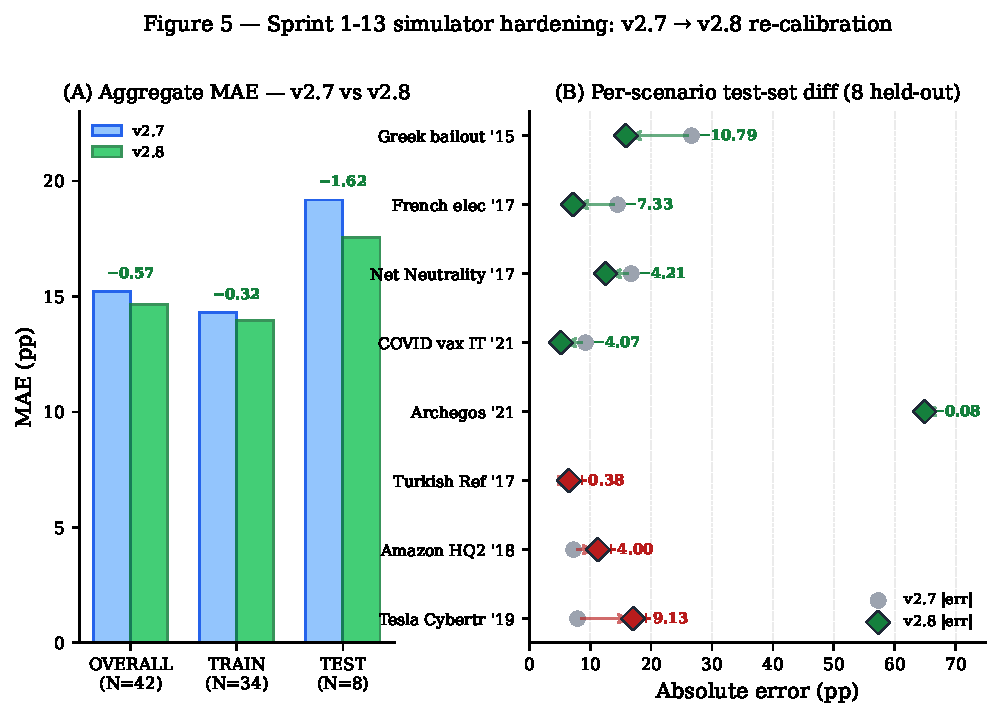
\includegraphics[width=\linewidth]{figures/fig5_v28_recalibration.pdf}
  \caption{Sprint 1-13 simulator hardening: v2.7 → v2.8 re-calibration.
    \textbf{(A)} Aggregate MAE on the same 42 empirical scenarios with
    identical SVI hyperparameters. \textbf{(B)} Per-scenario absolute
    error on the eight held-out test scenarios; arrows trace v2.7 → v2.8,
    green = improvement, red = regression. The four largest improvements
    correspond to scenarios (Greek 2015, French 2017, Net Neutrality
    2017, COVID vax IT 2021) where the country-alias and realism-gate
    fixes (sprints 6-7) reinstated previously-dropped stakeholders.}
  \label{fig:v28-recalibration}
\end{figure}

\subsubsection{10.4 Per-scenario test-set diff}\label{per-scenario-diff}

\begin{longtable}[]{@{}lllll@{}}
\toprule\noalign{}
Scenario & GT & v2.7 $|$err$|$ & v2.8 $|$err$|$ & $\Delta$ \\
\midrule\noalign{}
\endhead
Greek bailout (2015)     & 38.7 & 26.63 & 15.84 & $-10.78$ ✓ \\
French election (2017)   & 66.1 & 14.50 &  7.17 & $-7.32$ ✓ \\
Net Neutrality (2017)    & 83.0 & 16.74 & 12.53 & $-4.21$ ✓ \\
COVID vax IT (2021)      & 80.0 &  9.24 &  5.17 & $-4.07$ ✓ \\
Archegos Capital (2021)  & 35.0 & 65.00 & 64.92 & $-0.07$ ✓ \\
Turkish Ref. (2017)      & 51.4 &  6.11 &  6.49 & $+0.38$ ✗ \\
Amazon HQ2 (2018)        & 56.0 &  7.27 & 11.27 & $+3.99$ ✗ \\
Tesla Cybertruck (2019)  & 62.0 &  7.91 & 17.04 & $+9.13$ ✗ \\
\bottomrule\noalign{}
\end{longtable}

The four largest improvements are scenarios where the country-alias and
realism-gate fixes (sprints 6-7) reinstated previously dropped
stakeholders. The two regressions (Tesla Cybertruck, Amazon HQ2) are
flagged for v2.9 follow-up.

\subsubsection{10.5 Scope of unchanged
results}\label{scope-unchanged}

The apples-to-apples sim-lift evaluation (Section 6.10.4), the
contamination probe, the blinding protocol, the EnKF assimilation
result on Brexit, and the null-baseline benchmark all use trajectory
data and bench harness code that are independent of the simulator
calibration; their numbers carry through unchanged from v2.7. The
headline scientific claim --- that the calibrated ABM matches but does
not dominate naive persistence in retrospective trajectory space, and
earns its operational value from EnKF online assimilation plus its
blinding / benchmarking instrumentation --- is unaffected by v2.8.

\begin{center}\rule{0.5\linewidth}{0.5pt}\end{center}

\ldots{} --\textgreater{}

\section{Online Supplementary
Material}\label{online-supplementary-material}

The following appendices accompany the main manuscript as Online
Supplementary Material (SI). They are referenced from the main text as
``Appendix A'', ``Appendix B'', etc., but are not required to follow the
main argument. SI inclusion is for reproducibility and JASSS-mandated
documentation completeness:

\begin{itemize}
\tightlist
\item
  \textbf{Appendix A} --- implementation details (software stack,
  runtimes, gauge fixing, EMA standardisation, engine/market-context
  decomposition).
\item
  \textbf{Appendix B} --- regime-switching crisis dynamics (preliminary;
  not included in the main calibration).
\item
  \textbf{Appendix C} --- full 43-scenario corpus list.
\item
  \textbf{Appendix D} --- reproducibility of the v2.5 benchmark layer.
\item
  \textbf{Appendix E} --- Layer 0 scope analyzer and realism gate.
\item
  \textbf{Appendix F} --- contamination probing, blinding protocol, and
  trajectory metrics.
\item
  \textbf{Appendix G} --- ODD protocol description (Grimm et al.~2020)
  for the simulation model.
\end{itemize}

The main text gives an abridged version of Table C.1 (training/test
domain composition) inline as Table 2 (Section 5.1); the full
per-scenario breakdown is reproduced in Appendix C.1 of this supplement.

\subsection{Appendix A: Implementation
Details}\label{appendix-a-implementation-details}

\subsubsection{A.1 Software Stack}\label{a.1-software-stack}

The simulator and inference pipeline are implemented in Python using: -
\textbf{JAX} (0.9+) for differentiable simulation and automatic
differentiation. - \textbf{NumPyro} for probabilistic programming and
variational inference. - \textbf{SALib} for Sobol sensitivity analysis.
- All simulation code is \texttt{jax.jit}-compatible and uses
\texttt{jax.lax.scan} for sequential round stepping, avoiding Python
loops. - \textbf{Market data layer (v2.7)}: \texttt{yfinance} for
equity/volatility/yield feeds (VIX, UST 10Y and 5Y), a lightweight ECB
SDMX JSON client for euro-area long-term interest rates (IT/DE/AAA), and
the FRED public API for US corporate OAS (\texttt{BAMLC0A0CM}) and UK
10Y long-term interest rate (\texttt{IRLTLT01GBM156N}). Concurrent
fan-out is handled by \texttt{concurrent.futures.ThreadPoolExecutor}
(three workers, one per source), with a 300-second TTL cache on a
composite key and silent fallback to calibrated static priors on fetch
failure.

\subsubsection{A.2 Computational
Requirements}\label{a.2-computational-requirements}

\begin{longtable}[]{@{}
  >{\raggedright\arraybackslash}p{(\linewidth - 4\tabcolsep) * \real{0.3333}}
  >{\raggedright\arraybackslash}p{(\linewidth - 4\tabcolsep) * \real{0.3333}}
  >{\raggedright\arraybackslash}p{(\linewidth - 4\tabcolsep) * \real{0.3333}}@{}}
\toprule\noalign{}
\begin{minipage}[b]{\linewidth}\raggedright
Task
\end{minipage} & \begin{minipage}[b]{\linewidth}\raggedright
Runtime
\end{minipage} & \begin{minipage}[b]{\linewidth}\raggedright
Hardware
\end{minipage} \\
\midrule\noalign{}
\endhead
\bottomrule\noalign{}
\endlastfoot
SVI calibration (3000 steps, 42 scenarios) & 40.2 min & CPU (Apple
Silicon) \\
SBC (100 instances, NUTS) & 5.0 min & CPU \\
Sobol analysis (18,432 evaluations) & \textasciitilde10 min & CPU \\
SVI vs NUTS comparison (4 scenarios) & \textasciitilde15 min & CPU \\
EnKF online assimilation (50 members, 9 rounds) & \textasciitilde5 sec &
CPU \\
\end{longtable}

\subsubsection{A.3 Gauge Fixing}\label{a.3-gauge-fixing}

The softmax function is shift-invariant: softmax(α + c) = softmax(α) for
any scalar c.~With 5 forces and 4 free parameters, one weight must be
fixed to resolve the gauge. We fix α\_direct = 0, making the remaining
weights interpretable as log-odds ratios relative to direct LLM
influence. This is analogous to the reference category in multinomial
logistic regression.

\subsubsection{A.4 EMA Standardization}\label{a.4-ema-standardization}

The EMA standardization computes per-force, per-round statistics (mean
and standard deviation) across ALL agents in each round, accumulated via
exponential moving average over rounds with decay α = 0.3. The
current-round statistics are:

\[\mu_k^{\text{cur}}(t) = \frac{1}{n}\sum_i f_{k,i}(t), \quad \sigma_k^{\text{cur}}(t) = \sqrt{\frac{1}{n}\sum_i (f_{k,i}(t) - \mu_k^{\text{cur}})^2 + \epsilon}\]

The gradient-safe square root (adding ε = 10⁻⁸ before taking the root)
avoids NaN gradients when all agent forces are identical. These are then
smoothed temporally:

\[\mu_k(t) = \alpha \cdot \mu_k(t-1) + (1-\alpha) \cdot \mu_k^{\text{cur}}(t)\]

A permutation invariance test confirms that agent ordering does not
affect the standardized forces (max absolute difference \textless{} 6 ×
10⁻⁸ under random permutation of the agent array). This property holds
because mean and variance are symmetric statistics over the agent set.

\subsubsection{A.5 Engine Decomposition and Market-Context Dependency
Injection
(v2.7)}\label{a.5-engine-decomposition-and-market-context-dependency-injection-v2.7}

Two architectural changes were made in v2.7 that do not alter any
calibration, benchmark, or EnKF number in Sections 5--7 but are
prerequisites for the live market data layer of Section 5.9 and for the
per-scenario geography regimes used by the sovereign-spread and
local-index models.

\textbf{Engine decomposition.} The simulation entry point
(\texttt{core/simulation/engine.py}) was refactored from a 606-line God
Object that owned bootstrap, per-round stepping, evaluation, and
reporting into a thin 261-line coordinator and three
single-responsibility services: - \texttt{SimulationSetup}
(\texttt{core/simulation/setup.py}) --- scenario loading, agent roster
construction, market-context wiring, LLM client binding. -
\texttt{EvaluationService} (\texttt{core/simulation/evaluation.py}) ---
realism gate, scope analyzer, post-run diagnostic checks. -
\texttt{ReportingService} (\texttt{core/simulation/reporting.py}) ---
Markdown report and financial-impact JSON export.

The coordinator now holds only the per-round loop and delegates all
other responsibilities to these services. This eliminates several latent
bugs previously masked by a generic \texttt{except} block in engine
initialization (one of them, a silently swallowed \texttt{TypeError}
when \texttt{FinancialImpactScorer} was missing the
\texttt{relevant\_universe} kwarg, is fixed in the same commit).

\textbf{Market-context dependency injection.} The process-wide
\texttt{UniverseLoader} singleton, which had held the stock universe,
sector beta tables, and macro priors as module-level state, is replaced
by a per-scenario \texttt{MarketContext} object
(\texttt{core/orchestrator/market\_context.py}) bound at bootstrap time
to a geography regime (IT, US, EU, EM, default) and a
\texttt{MarketDataProvider} backend (static, live, or test).
\texttt{MarketContext} exposes two dedicated models ---
\texttt{SovereignSpreadModel} (BTP-Bund and analogous sovereign-spread
regressions, parameterised by geography) and \texttt{LocalIndexModel}
(primary local equity index and its political sensitivity, e.g.~FTSE MIB
for IT, S\&P 500 for US) --- which replace the previously hard-coded
BTP-Bund and FTSE MIB constants scattered across the financial impact
scorer. The \texttt{stock\_universe.json} schema gains a \texttt{macro}
block that declares calibrated base values and sensitivities for the six
supported geographies.

The consequence for downstream callers is that
\texttt{TickerRelevanceScorer}, \texttt{FinancialImpactScorer}, and
\texttt{backtest\_financials.py} all receive \texttt{MarketContext} via
constructor injection rather than reading from a global; tests can
inject a fake provider; and the live-feed overlay of Section 5.9 is
implemented by swapping the provider rather than patching a singleton.

\begin{center}\rule{0.5\linewidth}{0.5pt}\end{center}

\subsection{Appendix B: Regime Switching for Crisis Dynamics
(Preliminary)}\label{appendix-b-regime-switching-for-crisis-dynamics-preliminary}

\subsubsection{B.1 Motivation}\label{b.1-motivation}

The five worst-performing scenarios (Section 5.5) share a common
pattern: rapid, discontinuous opinion shifts that the base model's
linear force combination cannot reproduce. Financial crises (WeWork b\_s
= -1.378, SVB b\_s = -0.835, FTX b\_s = -0.727) exhibit trust collapses
where public opinion drops precipitously within 1--2 rounds. The base
model, with its smooth force mixing and capped step sizes, can only
produce gradual movements.

We address this with a regime-switching extension that introduces a
latent ``crisis regime'' with amplified dynamics, activated by
observable signals (shock magnitude, position velocity, institutional
trust).

\subsubsection{B.2 Two-Regime
Architecture}\label{b.2-two-regime-architecture}

The model switches between two regimes:

\begin{itemize}
\tightlist
\item
  \textbf{Regime 0 (Normal)}: Standard force-based opinion evolution as
  described in Section 3.
\item
  \textbf{Regime 1 (Crisis)}: Amplified step sizes, suppressed anchor
  rigidity, amplified herd and event forces, and a direct crisis push
  that bypasses the softmax mixing entirely.
\end{itemize}

The switching is \emph{soft}: regime probability P(crisis) ∈ (0, 1) is
computed via sigmoid, and all parameters are interpolated:

\[\boldsymbol{\theta}_{\text{eff}} = (1 - p) \cdot \boldsymbol{\theta}_{\text{normal}} + p \cdot \boldsymbol{\theta}_{\text{crisis}} \quad \text{(Eq. B.1)}\]

This preserves JAX differentiability and \texttt{jax.lax.scan}
compatibility---no discrete branching is needed.

\subsubsection{B.3 Regime Probability}\label{b.3-regime-probability}

The crisis probability is computed via logistic regression on four
observable signals:

\[\text{logit}(c_t) = \beta_0 + \beta_{\text{shock}} (m_t - \tau_{\text{shock}}) + \beta_{\text{vel}} (v_t - \tau_{\text{vel}}) + \beta_{\text{trust}} (1 - \text{trust}) + \beta_{\text{recovery}} \cdot r_t + \beta_{\text{momentum}} \cdot c_{t-1} \quad \text{(Eq. B.2)}\]

where m\_t is the shock magnitude, v\_t the mean absolute position
velocity, trust the scenario-level institutional trust, r\_t a soft
count of crisis rounds, and p\_\{t-1\} the previous crisis probability.

\subsubsection{B.4 Crisis Dynamics}\label{b.4-crisis-dynamics}

In the crisis regime, three modifications occur:

\begin{enumerate}
\def\labelenumi{\arabic{enumi}.}
\tightlist
\item
  \textbf{Step size amplification.} λ\_crisis = λ\_normal × 3.0, with
  relaxed caps.
\item
  \textbf{Force reweighting.} Herd amplified by log(2.0), event
  amplified by log(2.5), anchor suppressed by -2.0 in logit space.
\item
  \textbf{Direct crisis push.} A force that bypasses the softmax mixing:
  Δp\_i\^{}\{crisis\} = p · κ · m\_t · d\_t · (1 - ρ\_i), where κ = 0.4.
\end{enumerate}

\textbf{Table B.1: Crisis Parameter Defaults}

\begin{longtable}[]{@{}lll@{}}
\toprule\noalign{}
Parameter & Default & Role \\
\midrule\noalign{}
\endhead
\bottomrule\noalign{}
\endlastfoot
λ\_multiplier & 3.0 & Step size amplification in crisis \\
anchor\_suppression & 0.1 & Anchor force multiplied by this in crisis \\
event\_amplification & 2.5 & Event force amplified in softmax \\
herd\_amplification & 2.0 & Herd force amplified in softmax \\
contagion\_speed (κ) & 0.4 & Direct crisis push strength \\
shock\_trigger (τ\_shock) & 0.5 & Shock magnitude threshold \\
trust\_sensitivity & 1.5 & Low trust → higher crisis probability \\
crisis\_duration\_mean & 2.5 & Expected rounds before recovery \\
\end{longtable}

\subsubsection{B.5 Results}\label{b.5-results}

We compare the base model (v2) against the regime-switching model (v3)
on selected financial and corporate scenarios:

\textbf{Table B.2: v2 vs v3 on Financial/Corporate Scenarios}

\begin{longtable}[]{@{}
  >{\raggedright\arraybackslash}p{(\linewidth - 12\tabcolsep) * \real{0.1429}}
  >{\raggedright\arraybackslash}p{(\linewidth - 12\tabcolsep) * \real{0.1429}}
  >{\raggedright\arraybackslash}p{(\linewidth - 12\tabcolsep) * \real{0.1429}}
  >{\raggedright\arraybackslash}p{(\linewidth - 12\tabcolsep) * \real{0.1429}}
  >{\raggedright\arraybackslash}p{(\linewidth - 12\tabcolsep) * \real{0.1429}}
  >{\raggedright\arraybackslash}p{(\linewidth - 12\tabcolsep) * \real{0.1429}}
  >{\raggedright\arraybackslash}p{(\linewidth - 12\tabcolsep) * \real{0.1429}}@{}}
\toprule\noalign{}
\begin{minipage}[b]{\linewidth}\raggedright
Scenario
\end{minipage} & \begin{minipage}[b]{\linewidth}\raggedright
GT (\%)
\end{minipage} & \begin{minipage}[b]{\linewidth}\raggedright
v2 Error
\end{minipage} & \begin{minipage}[b]{\linewidth}\raggedright
v3 Error
\end{minipage} & \begin{minipage}[b]{\linewidth}\raggedright
Δ (pp)
\end{minipage} & \begin{minipage}[b]{\linewidth}\raggedright
Max P(crisis)
\end{minipage} & \begin{minipage}[b]{\linewidth}\raggedright
Crisis Rounds
\end{minipage} \\
\midrule\noalign{}
\endhead
\bottomrule\noalign{}
\endlastfoot
Dieselgate & 32.0 & 29.6 & 0.4 & +29.1 & 0.930 & 3 \\
FTX Crypto & 22.0 & 11.4 & 5.3 & +6.0 & 1.000 & 2 \\
Facebook→Meta & 26.0 & 14.6 & 6.4 & +8.2 & 0.911 & 2 \\
Archegos & 35.0 & 65.0 & 54.5 & +10.4 & 0.930 & 2 \\
Boeing 737 MAX & 40.0 & 9.5 & 23.7 & -14.2 & 0.833 & 1 \\
SVB Collapse & 38.0 & 38.8 & 61.9 & -23.1 & 0.989 & 2 \\
Twitter/X & 41.0 & 7.8 & 25.5 & -17.7 & 0.826 & 2 \\
\end{longtable}

Results are mixed. Regime switching produces substantial improvements
when crisis dynamics align with shock direction but degrades performance
when the crisis push amplifies the wrong direction. The high max
P(crisis) across all scenarios (0.67--1.0) with default thresholds
suggests the trigger is too sensitive and requires calibration via SVI.

\subsubsection{B.6 Design for
Calibration}\label{b.6-design-for-calibration}

The crisis parameters are designed to be learnable within the
hierarchical framework. The v3 model extends the v2 prior with 5
additional global parameters (crisis\_lambda\_mult,
crisis\_anchor\_supp, crisis\_event\_amp, crisis\_herd\_amp,
shock\_trigger), shared globally as crisis dynamics are hypothesized to
be a universal mechanism modulated by scenario-specific triggers.

\begin{center}\rule{0.5\linewidth}{0.5pt}\end{center}

\subsection{Appendix C: Full Scenario
List}\label{appendix-c-full-scenario-list}

\textbf{Table C.1: Full Empirical Dataset (43 scenarios)}

\emph{Scenario counts used in this paper.} The SVI calibration (Sections
4--5) and the multi-modal extension (Section 5.8) are fit on the first
42 scenarios (v2.5 training corpus). The v2.5 predictive-skill
benchmarks (Sections 6.6--6.8), the v2.7 contamination probe (Section
6.10), and the blinding A/B (Section 6.10.3) use the full 43-scenario
corpus, which adds
\texttt{CORP-2020-BOEING\_737\_MAX\_RETURN\_TO\_SERVICE} for evaluation
only. The SVI posterior is not re-fit on the 43rd scenario in this
version of the paper.

\begin{longtable}[]{@{}
  >{\raggedright\arraybackslash}p{(\linewidth - 14\tabcolsep) * \real{0.1250}}
  >{\raggedright\arraybackslash}p{(\linewidth - 14\tabcolsep) * \real{0.1250}}
  >{\raggedright\arraybackslash}p{(\linewidth - 14\tabcolsep) * \real{0.1250}}
  >{\raggedright\arraybackslash}p{(\linewidth - 14\tabcolsep) * \real{0.1250}}
  >{\raggedright\arraybackslash}p{(\linewidth - 14\tabcolsep) * \real{0.1250}}
  >{\raggedright\arraybackslash}p{(\linewidth - 14\tabcolsep) * \real{0.1250}}
  >{\raggedright\arraybackslash}p{(\linewidth - 14\tabcolsep) * \real{0.1250}}
  >{\raggedright\arraybackslash}p{(\linewidth - 14\tabcolsep) * \real{0.1250}}@{}}
\toprule\noalign{}
\begin{minipage}[b]{\linewidth}\raggedright
\#
\end{minipage} & \begin{minipage}[b]{\linewidth}\raggedright
Scenario ID
\end{minipage} & \begin{minipage}[b]{\linewidth}\raggedright
Domain
\end{minipage} & \begin{minipage}[b]{\linewidth}\raggedright
GT (\%)
\end{minipage} & \begin{minipage}[b]{\linewidth}\raggedright
Rounds
\end{minipage} & \begin{minipage}[b]{\linewidth}\raggedright
Polls
\end{minipage} & \begin{minipage}[b]{\linewidth}\raggedright
Split
\end{minipage} & \begin{minipage}[b]{\linewidth}\raggedright
Notes
\end{minipage} \\
\midrule\noalign{}
\endhead
\bottomrule\noalign{}
\endlastfoot
1 & COM-2017-IPHONE\_X & commercial & 65.0 & 5 & 2/5 & Train & \\
2 & COM-2019-TESLA\_CYBERTRUCK\_REVEAL & commercial & 62.0 & 7 & 1/7 &
Test & \\
3 & CORP-2015-DIESELGATE\_VW & corporate & 32.0 & 5 & 1/5 & Train & \\
4 & CORP-2017-UBER\_LONDON\_LICENSE & corporate & 65.0 & 9 & 1/9 & Train
& \\
5 & CORP-2017-UNITED\_AIRLINES\_DRAGGING & corporate & 28.0 & 6 & 1/6 &
Train & \\
6 & CORP-2018-AMAZON\_HQ2\_NYC & corporate & 56.0 & 7 & 1/7 & Test & \\
7 & CORP-2019-BOEING\_737\_MAX & corporate & 40.0 & 7 & 1/7 & Train & \\
7a & CORP-2020-BOEING\_737\_MAX\_RETURN\_TO\_SERVICE & corporate & 41.0
& 5 & 5/5 & Eval-only & v2.7 addition (benchmark / contamination
only) \\
8 & CORP-2021-FACEBOOK\_META\_REBRAND & corporate & 26.0 & 7 & 1/7 &
Train & \\
9 & CORP-2022-TWITTER\_X\_ACQUISITION & corporate & 41.0 & 5 & 1/5 &
Train & \\
10 & ENE-2012-JAPANESE\_NUCLEAR\_RESTART & energy & 35.0 & 6 & 4/6 &
Train & \\
11 & ENV-2018-GRETA\_CLIMATE\_STRIKES & environmental & 71.0 & 6 & 0/6 &
Train & \\
12 & FIN-2019-WEWORK\_IPO\_COLLAPSE & financial & 18.0 & 7 & 1/7 & Train
& \\
13 & FIN-2020-TESLA\_STOCK\_SPLIT & financial & 72.0 & 7 & 0/7 & Train
& \\
14 & FIN-2021-AMC\_SHORT\_SQUEEZE & financial & 62.0 & 7 & 0/7 & Train
& \\
15 & FIN-2021-ARCHEGOS\_CAPITAL\_COLLAPSE & financial & 35.0 & 7 & 0/7 &
Test & NEEDS\_VERIF \\
16 & FIN-2021-GAMESTOP & financial & 72.0 & 7 & 1/7 & Train & \\
17 & FIN-2022-FTX\_CRYPTO\_CRISIS & financial & 22.0 & 7 & 2/7 & Train
& \\
18 & FIN-2023-SVB\_COLLAPSE & financial & 38.0 & 6 & 2/6 & Train & \\
19 & LAB-2015-UBER\_VS\_TAXI\_FRANCE & labor & 45.0 & 7 & 2/7 & Train
& \\
20 & PH-2021-ASTRAZENECA\_HESITANCY & public\_health & 62.0 & 7 & 0/7 &
Train & \\
21 & PH-2021-COVID\_VAX\_IT & public\_health & 80.0 & 7 & 7/7 & Test
& \\
22 & PH-2021-MASKING\_MANDATE\_USA & public\_health & 63.0 & 5 & 2/5 &
Train & \\
23 & PH-2021-VACCINE\_HESITANCY\_USA & public\_health & 67.0 & 5 & 5/5 &
Train & \\
24 & PH-2022-MONKEYPOX\_CONCERN\_USA & public\_health & 47.0 & 7 & 1/7 &
Train & \\
25 & POL-2011-REFERENDUM\_DIVORZIO\_MALTA & political & 53.2 & 6 & 0/6 &
Train & \\
26 & POL-2014-SCOTTISH\_INDEPENDENCE & political & 44.7 & 7 & 7/7 &
Train & \\
27 & POL-2015-GREEK\_BAILOUT\_GREXIT & political & 38.7 & 5 & 0/5 & Test
& \\
28 & POL-2016-BREXIT & political & 51.9 & 6 & 6/6 & Train & \\
29 & POL-2016-REFERENDUM\_COSTITUZIONALE\_IT & political & 40.9 & 7 &
0/7 & Train & \\
30 & POL-2017-PRESIDENZIALI\_FRANCIA & political & 66.1 & 6 & 6/6 & Test
& \\
31 & POL-2017-INDIPENDENZA\_CATALOGNA & political & 48.0 & 5 & 1/5 &
Train & \\
32 & POL-2017-TURKISH\_CONSTITUTIONAL\_REF & political & 51.4 & 6 & 0/6
& Test & \\
33 & POL-2018-USA\_MIDTERM\_HOUSE & political & 53.4 & 6 & 6/6 & Train
& \\
34 & POL-2018-REFERENDUM\_ABORTO\_IRLANDA & political & 66.4 & 6 & 3/6 &
Train & \\
35 & POL-2019-EUROPEE\_ITALIA & political & 40.0 & 6 & 6/6 & Train & \\
36 & POL-2020-CHILE\_CONSTITUTIONAL\_REF & political & 78.3 & 6 & 6/6 &
Train & \\
37 & POL-2020-PRESIDENZIALI\_USA & political & 51.3 & 7 & 7/7 & Train
& \\
38 & POL-2022-PRESIDENZIALI\_BRASILE & political & 50.9 & 6 & 6/6 &
Train & \\
39 & SOC-2017-AUSTRALIA\_SAME\_SEX\_MARRIAGE & social & 61.6 & 7 & 7/7 &
Train & \\
40 & TECH-2017-NET\_NEUTRALITY\_REPEAL\_US & technology & 83.0 & 5 & 1/5
& Test & \\
41 & TECH-2018-GDPR\_ADOPTION & technology & 67.0 & 7 & 0/7 & Train & \\
42 & TECH-2020-TIKTOK\_US\_BAN\_DEBATE & technology & 60.0 & 6 & 1/6 &
Train & \\
\end{longtable}

Total: 43 scenarios (42 SVI corpus + 1 eval-only v2.7 addition). SVI
split: 34 train / 8 test. 10 domains. 1 flagged NEEDS\_VERIFICATION
(Archegos). 14 enriched with financial market data (all FIN-* and CORP-*
scenarios). Verified polling available for 31 scenarios (polling from
LLM estimation where sample\_size is not verified). Median scenario
length: 6 rounds.

Note: Scenario IDs are abbreviated in the table for readability. Full
IDs are available in the repository. The ``Polls'' column shows rounds
with verified sample sizes vs.~total rounds. Ground truth sources
include official election results, certified referendum outcomes, and
verified survey data.

\begin{center}\rule{0.5\linewidth}{0.5pt}\end{center}

\subsection{Appendix D: Reproducibility of the v2.5 Benchmark
Layer}\label{appendix-d-reproducibility-of-the-v2.5-benchmark-layer}

All numerical results in Sections 6.6--6.8 are produced by a
self-contained Python module released alongside the codebase. This
appendix documents the package, its command-line interface, and its
automated test suite so that the reference distribution can be rederived
from scratch and any modification to the sim can be re-evaluated against
it.

\subsubsection{D.1 Module Layout}\label{d.1-module-layout}

The \texttt{benchmarks/} package contains six first-class modules:

\begin{longtable}[]{@{}
  >{\raggedright\arraybackslash}p{(\linewidth - 2\tabcolsep) * \real{0.2727}}
  >{\raggedright\arraybackslash}p{(\linewidth - 2\tabcolsep) * \real{0.7273}}@{}}
\toprule\noalign{}
\begin{minipage}[b]{\linewidth}\raggedright
File
\end{minipage} & \begin{minipage}[b]{\linewidth}\raggedright
Responsibility
\end{minipage} \\
\midrule\noalign{}
\endhead
\bottomrule\noalign{}
\endlastfoot
\texttt{forecasters.py} & Closed-form null baselines: naive persistence,
running mean, OLS linear trend, AR(1). Exposes
\texttt{generate\_baseline\_trajectory} for one-step-ahead rolling
forecasts and \texttt{forecast\_errors} / \texttt{rmse} helpers. \\
\texttt{diebold\_mariano.py} & DM statistic with the
Harvey--Leybourne--Newbold correction. Student-\(t\) p-values computed
via the regularized incomplete beta identity
\(P(T > x) = \tfrac{1}{2} I_{\nu/(\nu+x^2)}(\nu/2, 1/2)\) with Lentz's
continued-fraction expansion --- no SciPy dependency. \\
\texttt{coverage.py} & Empirical coverage of an interval sequence
against realized values, plus a nonparametric bootstrap confidence band
on the coverage statistic itself. Includes a
\texttt{coverage\_from\_quantiles} helper for ensemble Monte Carlo
intervals. \\
\texttt{residual\_ci.py} & Residual-bootstrap predictive intervals that
turn any point-forecaster into a calibrated interval forecaster,
enabling the model-free coverage check of Section 6.7. \\
\texttt{scenario\_matrix.py} & Enumeration of the
\(7 \times 5 \times 4\) scenario-diversity axis, \texttt{ScenarioCell}
dataclass, and a \texttt{coverage\_report} that flags missing axis
values in any given corpus. \\
\texttt{historical.py} / \texttt{historical\_runner.py} & Loader that
normalizes the v1 and v2.2 empirical JSON scenarios into the common
\texttt{support} / \texttt{signed\_position} representation, derives
tension from per-scenario volatility, maps ISO country codes to regions,
and runs all baselines + DM tests + coverage + matrix report in one
pass. \\
\texttt{runner.py} & Parallel runner for the deterministic-trajectory
benchmark against the 7 scenarios stored in
\texttt{frontend/public/data/scenario\_*} (the sim-forecast case). \\
\end{longtable}

\subsubsection{D.2 Command-Line Usage}\label{d.2-command-line-usage}

The historical benchmark (Section 6.6--6.8) regenerates from scratch
with:

\begin{Shaded}
\begin{Highlighting}[]
\ExtensionTok{python} \AttributeTok{{-}m}\NormalTok{ benchmarks.historical\_runner }\DataTypeTok{\textbackslash{}}
    \AttributeTok{{-}{-}out}\NormalTok{ outputs/historical\_benchmark.json }\DataTypeTok{\textbackslash{}}
    \AttributeTok{{-}{-}markdown}\NormalTok{ outputs/historical\_benchmark.md}
\end{Highlighting}
\end{Shaded}

The deterministic-trajectory benchmark (sim-forecast case, for
continuous regression testing) runs with:

\begin{Shaded}
\begin{Highlighting}[]
\ExtensionTok{python} \AttributeTok{{-}m}\NormalTok{ benchmarks }\DataTypeTok{\textbackslash{}}
    \AttributeTok{{-}{-}out}\NormalTok{ outputs/benchmark\_report.json }\DataTypeTok{\textbackslash{}}
    \AttributeTok{{-}{-}markdown}\NormalTok{ outputs/benchmark\_report.md}
\end{Highlighting}
\end{Shaded}

Both commands are zero-configuration on the public repository and write
machine-readable JSON + human-readable Markdown reports.

\subsubsection{D.3 Automated Test Suite}\label{d.3-automated-test-suite}

The benchmark layer ships with 103 automated tests distributed across
five files and four markers (\texttt{slow}, \texttt{integration},
\texttt{perf}, \texttt{stress}):

\begin{longtable}[]{@{}
  >{\raggedright\arraybackslash}p{(\linewidth - 4\tabcolsep) * \real{0.4074}}
  >{\raggedright\arraybackslash}p{(\linewidth - 4\tabcolsep) * \real{0.2593}}
  >{\raggedright\arraybackslash}p{(\linewidth - 4\tabcolsep) * \real{0.3333}}@{}}
\toprule\noalign{}
\begin{minipage}[b]{\linewidth}\raggedright
Test file
\end{minipage} & \begin{minipage}[b]{\linewidth}\raggedright
Tests
\end{minipage} & \begin{minipage}[b]{\linewidth}\raggedright
Purpose
\end{minipage} \\
\midrule\noalign{}
\endhead
\bottomrule\noalign{}
\endlastfoot
\texttt{test\_benchmarks.py} & 18 & Unit tests for forecasters, DM,
coverage, scenario matrix. \\
\texttt{test\_benchmarks\_integration.py} & 8 & End-to-end runner tests,
including residual-bootstrap calibration on i.i.d. noise. \\
\texttt{test\_performance\_sla.py} & 5 & Throughput SLAs for DM,
coverage, baselines, and the runner (defaults: 1000 DM tests in
\textless{} 5 s, runner on 20 synthetic scenarios in \textless{} 3 s).
All thresholds env-overridable via \texttt{DTS\_SLA\_*}. \\
\texttt{test\_stress\_scenarios.py} & 57 & Adversarial-signal stress
tests (flat, monotone, alternating, spike, heavy-tail, near-constant),
DM sign-consistency under \(a \leftrightarrow b\) swap, coverage
boundedness under random intervals, per-cell smoke tests on the full
scenario matrix. \\
\texttt{test\_historical\_benchmark.py} & 15 & Unit + integration tests
for the empirical loader (including v1/v2.2 duplicate resolution,
\texttt{None}-field tolerance, and domain-alias collapse) and the
aggregate runner. Includes a corpus smoke test that fails loudly if the
matrix coverage regresses. \\
\end{longtable}

Total runtime on a laptop-class machine: 2.94 seconds for the full
103-test suite, which is kept under 5 seconds so it can run on every
commit without gating.

\subsubsection{D.4 Release Artifacts}\label{d.4-release-artifacts}

Running the two commands above produces four reproducible artifacts
shipped with the paper:

\begin{enumerate}
\def\labelenumi{\arabic{enumi}.}
\tightlist
\item
  \texttt{outputs/historical\_benchmark.json} --- the full per-scenario
  × per-metric × per-baseline score matrix (43 × 2 × 4 = 344 score
  rows).
\item
  \texttt{outputs/historical\_benchmark.md} --- the human-readable
  summary from which Tables 15a, 15b, 16, and 17 are extracted verbatim.
\item
  \texttt{outputs/benchmark\_report.json} --- the
  deterministic-trajectory benchmark on the 7 scenarios currently
  shipped with the frontend, used as a continuous regression signal.
\item
  \texttt{outputs/benchmark\_report.md} --- the corresponding Markdown
  summary.
\end{enumerate}

Any future modification to the simulator, the calibration pipeline, or
the EnKF can be A/B-tested against the v2.5 reference distribution by
running the two commands before and after the change. Disagreement on
any DM cell at \(p < 0.05\) constitutes a reproducibility-relevant
regression.

\begin{center}\rule{0.5\linewidth}{0.5pt}\end{center}

\subsection{Appendix E: Layer 0 --- Scope Analyzer and Realism
Gate}\label{appendix-e-layer-0-scope-analyzer-and-realism-gate}

This appendix documents the pre-simulation realism layer introduced in
Section 6.9. Layer 0 is implemented in the \texttt{briefing/} package
and is wired into \texttt{ScenarioBuilder.build\_from\_brief()} upstream
of the agent generator.

\subsubsection{E.1 Scope Analyzer}\label{e.1-scope-analyzer}

The analyzer consumes the free-text brief and optional web-research
context and produces a typed \texttt{BriefScope}:

\begin{verbatim}
sector               : str   # snake_case; e.g. fashion_retail, industrial_lighting
sub_sector           : str   # optional narrower tag; empty when absent
geography            : list[str]     # ISO country codes or GLOBAL
scope_tier           : {global, national, regional, niche}
named_entities       : list[str]     # extracted verbatim from the brief
stakeholder_archetypes : list[str]   # whitelist (advisory, used downstream)
excluded_archetypes  : list[str]     # denylist (hard-blocked by gate)
language_register    : {formal, informal, technical}
rationale            : str           # one-sentence trace for logs
\end{verbatim}

The analyzer runs a single JSON-constrained LLM call with temperature
0.2 and a ≈1500-token output budget. It is deliberately
\textbf{person-name-free}: it defines the boundaries within which names
are later selected, to avoid mixing boundary definition and candidate
proposal in the same call.

\subsubsection{E.2 Realism Gate}\label{e.2-realism-gate}

After the multi-step agent generator (scaffold → elite → institutional →
clusters) proposes a roster, every candidate agent is fed, in batches of
12, to a verdict prompt that carries the \texttt{BriefScope} and returns
\texttt{\{verdict,\ rationale\}} per agent. The gate prompt has four
structural properties:

\begin{enumerate}
\def\labelenumi{\arabic{enumi}.}
\tightlist
\item
  \textbf{Whitelist is advisory, denylist is hard.} The prompt
  explicitly states ``Do not reject on archetype mismatch alone when
  sector and geography clearly fit.'' Conversely, any agent tagged with
  a denylisted archetype is a hard block.
\item
  \textbf{Explicit acceptance of institutional shapes.} Industry
  associations, academic institutions, trade bodies, regulators, and
  media outlets are acceptable even when their archetype label is absent
  from the whitelist, provided sector and geography fit.
\item
  \textbf{Composition hint.} A conditional block injected into the
  elite/institutional generator prompts (not the gate) prefers
  specialist voices when \texttt{sub\_sector} is set or
  \texttt{scope\_tier\ ∈\ \{niche,\ regional\}}; softens to ``include
  2--3 specialist voices alongside generalists'' otherwise. The hint is
  sector-name-free: it references the abstract pattern (specialist
  critic, community curator, newsletter author, sub-sector historian)
  rather than any concrete firm or figure.
\item
  \textbf{Batch-level failure safety.} If the gate LLM call fails for a
  batch, every agent in that batch is marked \texttt{uncertain} with
  rationale \texttt{gate\ LLM\ error}, not rejected. This prevents LLM
  flakiness from masquerading as realism signal.
\end{enumerate}

\subsubsection{E.3 Enforcement Loop}\label{e.3-enforcement-loop}

\texttt{enforce\_realism(scope,\ brief,\ analysis,\ llm,\ rejection\_threshold=0.15,\ max\_passes=2)}
wraps the gate in a regeneration loop:

\begin{enumerate}
\def\labelenumi{\arabic{enumi}.}
\tightlist
\item
  Run the gate on the current roster. If the rejection rate is ≤ τ =
  0.15, return.
\item
  Otherwise, identify rejected agents and call the generator's elite or
  institutional regeneration prompt with the rejection rationales
  appended as feedback.
\item
  Re-run the gate on the new candidates, up to \(P = 2\) passes total.
\item
  Return \texttt{(final\_report,\ initial\_report)} so downstream
  consumers can observe both the baseline and the post-enforcement
  rosters; both are serialized under \texttt{\_realism\_report} and
  \texttt{\_realism\_initial\_report} in the scenario config.
\end{enumerate}

The two thresholds \((\tau, P) = (0.15, 2)\) were chosen to bound cost:
\(P = 2\) caps the worst-case roster cost at roughly 3× the baseline
(one generation + two gate calls + one regen), and \(\tau = 0.15\) is
loose enough that a single borderline rejection on a 30-agent roster
does not force a regeneration pass.

\subsubsection{E.4 Test Coverage}\label{e.4-test-coverage}

Layer 0 ships with 38 automated tests distributed across two files:

\begin{longtable}[]{@{}
  >{\raggedright\arraybackslash}p{(\linewidth - 4\tabcolsep) * \real{0.4074}}
  >{\raggedright\arraybackslash}p{(\linewidth - 4\tabcolsep) * \real{0.2593}}
  >{\raggedright\arraybackslash}p{(\linewidth - 4\tabcolsep) * \real{0.3333}}@{}}
\toprule\noalign{}
\begin{minipage}[b]{\linewidth}\raggedright
Test file
\end{minipage} & \begin{minipage}[b]{\linewidth}\raggedright
Tests
\end{minipage} & \begin{minipage}[b]{\linewidth}\raggedright
Purpose
\end{minipage} \\
\midrule\noalign{}
\endhead
\bottomrule\noalign{}
\endlastfoot
\texttt{test\_layer0\_scope.py} & 19 & \texttt{BriefScope} dataclass
shape, prompt-block rendering, \texttt{analyze\_scope} happy-path and
edge cases, gate-prompt semantics (Phase 6 regressions: whitelist
advisory, denylist hard, industry bodies explicitly acceptable),
\texttt{run\_realism\_gate} end-to-end with mocked LLM. \\
\texttt{test\_layer0\_integration.py} & 19 & Composition-hint
narrow-vs-broad behavior (Phase 7 regressions, domain-neutrality check),
\texttt{enforce\_realism} multi-pass loop, \texttt{agent\_generator}
scope threading, \texttt{entity\_researcher} scope threading. \\
\end{longtable}

Total runtime: \textless{} 1 s on a laptop-class machine.

\subsubsection{E.5 Pilot-Brief
Telemetry}\label{e.5-pilot-brief-telemetry}

For reproducibility, the per-brief realism telemetry below is emitted by
\texttt{scripts/smoke\_layer0.py}:

\begin{verbatim}
Brief: "Stone Island lancia linea donna AW26"
  Scope : [niche] fashion_retail/luxury_streetwear in IT
  Gate  : pre=0.00 post=0.96  Rejected=1/26  Cost≈$0.03

Brief: "AEC Illuminazione viene acquisita da Signify"
  Scope : [national] industrial_lighting/smart_infrastructure_integration in IT,EU
  Gate  : pre=0.29 (8/34)  post=0.94 (31/34)  Rejected=1/34  Cost=$0.029
\end{verbatim}

A corpus-wide audit of the gate against the legacy rosters of all 43
in-scope empirical scenarios (no roster regeneration) is shipped as
\texttt{scripts/layer0\_corpus\_audit.py} and produces
\texttt{outputs/layer0\_corpus\_audit.\{json,md\}}. The audit costs
\$0.048 in LLM calls and runs in 39 s. Its results, summarised in
Section 6.9.1, motivate the v2.7 gate refactor (Section 8.3, item 11):
full back-application requires the context-aware denylist before
re-calibration is informative.

\begin{center}\rule{0.5\linewidth}{0.5pt}\end{center}

\subsection{Appendix F: Contamination Probing, Blinding Protocol, and
Trajectory Evaluation Metrics
(v2.7)}\label{appendix-f-contamination-probing-blinding-protocol-and-trajectory-evaluation-metrics-v2.7}

This appendix documents the implementation details of the
benchmark-integrity layer introduced in Section 6.10. The material is
split into four subsections: probe prompts and graders (F.1), blinding
transformations and sidecar format (F.2), the trajectory-evaluation
metrics library (F.3), and the reproducibility and cost envelope (F.4).

\subsubsection{F.1 Probe Prompts, Graders, and Confidence
Scaling}\label{f.1-probe-prompts-graders-and-confidence-scaling}

The contamination probe is implemented in
\texttt{benchmarks/contamination\_probe.py} and uses four prompt
templates, one per axis. All prompts share a single system instruction:

\begin{quote}
``You are a research assistant answering factual questions about public
events. Answer only in valid JSON matching the requested schema. If you
genuinely don't remember a fact, set the field to \texttt{null} rather
than guessing --- we are measuring recall, not creativity.''
\end{quote}

The asymmetric incentive (``null beats a wrong guess'') is the key to
separating memorization from confabulation: a model that confabulates
with high confidence is penalized because the grader still compares its
guess against ground truth, whereas a model that declines is simply
scored 0 on that axis without loss.

\textbf{Outcome axis.} Prompt asks for (i) whether the event is
recalled, (ii) the winning side (\texttt{"pro"} / \texttt{"against"} /
\texttt{null}), (iii) the final pro-side percentage, (iv) a confidence
score in \([0, 1]\). The grader computes
\(s = 0.4 \cdot \mathbb{1}[\text{winner match}] + 0.6 \cdot \mathbb{1}[|\hat{p}_{\text{pro}} - p_{\text{pro}}^{\text{gt}}| \leq 2 \text{pp}] + 0.3 \cdot \mathbb{1}[2 \text{pp} < |\hat{p}_{\text{pro}} - p_{\text{pro}}^{\text{gt}}| \leq 5 \text{pp}]\),
caps \(s\) at \(1.0\), and returns \(s \cdot \max(0.3, c)\) where \(c\)
is the model's confidence (the floor of \(0.3\) prevents a model from
trivially scoring zero by reporting zero confidence).

\textbf{Trajectory axis.} Prompt asks for the qualitative shape of the
polling movement (one of \texttt{"tightened"}, \texttt{"blew\_out"},
\texttt{"flat"}, \texttt{"reversed"}) and which side led early and late.
The ground-truth shape is computed from the empirical signed-position
trajectory: \texttt{flat} if
\(|p_{\text{late}} - p_{\text{early}}| < 0.05\), else \texttt{blew\_out}
if the late lead exceeds the early lead in absolute value, else
\texttt{tightened} if the late absolute position is smaller than the
early, else \texttt{reversed}. Score is
\(0.4 \cdot \mathbb{1}[\text{shape match}] + 0.3 \cdot \mathbb{1}[\text{early match}] + 0.3 \cdot \mathbb{1}[\text{late match}]\),
scaled by confidence.

\textbf{Events axis.} Prompt asks for up to three named campaign events
with approximate dates. Score is the token-overlap recall: for each
claimed event, its lowercased word tokens of length \(> 3\) are
intersected with the token set of each ground-truth event description; a
claimed event counts as matched if any ground-truth event has \(\geq 2\)
token overlap. Recall is
\(\text{matched} / \max(1, n_{\text{gt events}})\), capped at \(1.0\)
and scaled by confidence. This is deliberately lenient: partial-overlap
matches score full credit, which biases the probe toward flagging
\emph{more} contamination rather than missing it.

\textbf{Actors axis.} Prompt asks for up to three pro-side and three
against-side leaders. Ground truth is derived from the scenario's agent
roster: pro leaders are agents with
\texttt{initial\_position\ \textgreater{}\ +0.2}, against leaders are
agents with \texttt{initial\_position\ \textless{}\ -0.2}. Scoring uses
per-token intersection on names (tokens of length \(> 3\)), counting a
claimed actor as a hit if any token of any ground-truth actor on the
same side appears in the claim. Raw score is
\(\min(1.0, (\text{pro hits} + \text{against hits}) / 6)\), scaled by
confidence.

The per-scenario contamination index is
\(\text{idx} = \frac{2 \cdot s_{\text{outcome}} + s_{\text{trajectory}} + s_{\text{events}} + s_{\text{actors}}}{5}\).
Double-weighting outcome reflects the fact that recalling the final
result is the most direct form of leakage --- a model that knows who won
a referendum but not who campaigned for which side is still unusable as
a retrospective benchmark substrate.

\textbf{Grader caveats documented in
\texttt{outputs/contamination\_report.md}.} Three known limitations of
the grader are carried through to the report so a reader can adjust
their interpretation of the index:

\begin{enumerate}
\def\labelenumi{\arabic{enumi}.}
\tightlist
\item
  \emph{Pro/against semantic flip.} For the Brexit scenario, the dataset
  encodes \texttt{pro\ =\ Leave} (matching the reform-accept convention
  of the corpus) while colloquial usage would have
  \texttt{pro-Brexit\ =\ Leave} and therefore also \texttt{=\ pro}. The
  LLM's factually correct answer (``Leave won, \(\approx 52\%\)'') is
  graded as wrong when it uses the opposite convention. This understates
  Brexit's true contamination; it has no effect on the A/B comparison
  because the same convention is used in both arms.
\item
  \emph{Confidence scaling floor.} Multiplying raw scores by
  \(\max(0.3, c)\) rewards honest
  \texttt{I\ don\textquotesingle{}t\ know} answers but also means that a
  model which is \emph{right but unsure} looks less contaminated than it
  actually is. Contamination indices should be read as a lower bound on
  the model's actual recall.
\item
  \emph{Actor-matching leniency.} Word-token intersection scores
  partial-name overlaps as hits (e.g.~``Boris'' hitting ``Boris
  Johnson''), which tends to reward memorized surnames over full-name
  recall. This makes the actors axis slightly optimistic toward
  contamination detection --- a feature, not a bug, for the purposes of
  conservative benchmark design.
\end{enumerate}

\subsubsection{F.2 Blinding Transformations and Sidecar
Format}\label{f.2-blinding-transformations-and-sidecar-format}

\texttt{benchmarks/blinding.py} implements the five transformation steps
of Section 6.10.2 as a deterministic pure function
\texttt{blind\_scenario(raw:\ dict)\ -\textgreater{}\ (blinded:\ dict,\ bmap:\ BlindingMap)}.
The blinded dict has the following field-by-field contract with the
input:

\begin{longtable}[]{@{}
  >{\raggedright\arraybackslash}p{(\linewidth - 4\tabcolsep) * \real{0.3404}}
  >{\raggedright\arraybackslash}p{(\linewidth - 4\tabcolsep) * \real{0.3191}}
  >{\raggedright\arraybackslash}p{(\linewidth - 4\tabcolsep) * \real{0.3404}}@{}}
\toprule\noalign{}
\begin{minipage}[b]{\linewidth}\raggedright
original field
\end{minipage} & \begin{minipage}[b]{\linewidth}\raggedright
blinded field
\end{minipage} & \begin{minipage}[b]{\linewidth}\raggedright
transformation
\end{minipage} \\
\midrule\noalign{}
\endhead
\bottomrule\noalign{}
\endlastfoot
\texttt{id} & \texttt{id} &
\texttt{"BLINDED\_"\ +\ sha1(original\_id){[}:10{]}} \\
\texttt{id} & \texttt{original\_id} & \textbf{retained} (bookkeeping
only; never read by the sim) \\
\texttt{title} & \texttt{title} & template:
\texttt{f"Binary\ \{domain\}\ referendum-style\ decision\ over\ \{n\}\ polling\ rounds"} \\
\texttt{country} & \texttt{country} &
\(\text{"Country\_"} + \text{sha1}(\text{country}.\text{upper}())[:2]\) \\
\texttt{date\_start}, \texttt{date\_end} & \texttt{date\_start\_rel},
\texttt{date\_end\_rel} & \(T - N d\) (relative to
\texttt{date\_end}) \\
\texttt{n\_rounds}, \texttt{round\_duration\_days} & same &
\textbf{unchanged} \\
\texttt{ground\_truth\_outcome} & same & \textbf{unchanged} (grader
only) \\
\texttt{polling\_trajectory} & \texttt{polling\_trajectory} & per-round
\texttt{pro\_pct}, \texttt{against\_pct}, \texttt{undecided\_pct}
unchanged; \texttt{date} rewritten as \texttt{T-N\ d} \\
\texttt{events} & \texttt{events} & per-event \texttt{shock\_magnitude},
\texttt{shock\_direction}, \texttt{round} unchanged;
\texttt{description} scrubbed; \texttt{date} rewritten \\
\texttt{agents} & \texttt{agents} & \texttt{initial\_position},
\texttt{influence}, \texttt{type} unchanged; \texttt{name} replaced with
role-rank alias; \texttt{description} scrubbed \\
\texttt{covariates} & same & \textbf{unchanged} \\
\end{longtable}

The sidecar map stored at
\texttt{calibration/empirical/blinding\_maps/\textless{}id\textgreater{}.map.json}
contains the original title, original country, original date\_end, and
the full alias→original table. This file is read only by the grader at
benchmark-scoring time; the simulator's prompts never include any field
from the sidecar.

The \texttt{\_scrub(text,\ rename\_map)} function applies three passes
to every free-text field:

\begin{enumerate}
\def\labelenumi{\arabic{enumi}.}
\tightlist
\item
  \textbf{Named-entity substitution.} The rename map (plus its
  token-split expansion, see Section 6.10.2) is applied as a sequence of
  word-boundary regexes, processed in descending order of key length so
  that longer names win over their token subsets.
\item
  \textbf{Stoplist substitution.} A fixed dictionary of \(\sim 50\)
  geography and political-lexicon tokens (see \texttt{STOPLIST} in
  \texttt{benchmarks/blinding.py}) is applied with the same
  word-boundary discipline. Entries mapping to an empty string are
  removed; others are replaced with a category token.
\item
  \textbf{Year scrubbing.} The regex
  \texttt{\textbackslash{}b(19\textbar{}20)\textbackslash{}d\{2\}\textbackslash{}b}
  is replaced with the literal string \texttt{YEAR}.
\end{enumerate}

The function is deterministic: given the same input
\texttt{(text,\ rename\_map)} it returns the same output. This
determinism is verified indirectly by the fact that
\texttt{python\ -m\ benchmarks.blinding} is idempotent --- re-running it
produces byte-identical files.

\subsubsection{F.3 Trajectory Evaluation Metrics
Library}\label{f.3-trajectory-evaluation-metrics-library}

\texttt{benchmarks/eval\_metrics.py} provides a compact, dependency-free
library used by the sim-vs-ground-truth comparison step (Section 8.3,
item 13). The library exposes:

\begin{itemize}
\tightlist
\item
  \texttt{dtw\_distance(a,\ b)} --- dynamic time warping with
  absolute-difference pointwise cost, rolling two-row DP,
  \(O(n \cdot m)\) time and \(O(\min(n, m))\) space. Returns the
  accumulated misalignment in input units (not squared).
\item
  \texttt{normalized\_dtw(a,\ b)} --- DTW divided by \(\max(|a|, |b|)\),
  so values from scenarios with different round counts are comparable.
\item
  \texttt{ks\_statistic(a,\ b)} --- two-sample Kolmogorov--Smirnov \(D\)
  between the empirical CDFs, without the associated p-value. Used to
  measure marginal-distribution disagreement between a forecast
  trajectory and a ground-truth trajectory independent of round-count
  alignment.
\item
  \texttt{rmse(a,\ b)} --- mean-squared error over the shortest prefix
  shared by both inputs.
\item
  \texttt{terminal\_error(forecast,\ gt\_value)} --- absolute error of
  the forecast's final round against a verified terminal ground-truth.
\item
  \texttt{bootstrap\_ci(values,\ n\_samples=2000,\ ci=0.95,\ seed=42)}
  --- percentile bootstrap CI on the mean, deterministic via a seeded
  \texttt{random.Random}.
\item
  \texttt{compare\_trajectories(forecast,\ ground\_truth,\ terminal\_gt=None)}
  --- convenience function returning a \texttt{TrajectoryComparison}
  dataclass with all of the above.
\end{itemize}

DTW is the primary metric because the simulator produces trajectories on
its own internal schedule and polling observations are irregularly
timed; RMSE punishes time-warp even when shapes match, while DTW is
invariant to local time-axis stretching. KS provides a
distribution-level check that complements DTW at the sequence level.
Bootstrap CI on error, combined with the existing Diebold--Mariano
machinery in \texttt{benchmarks/diebold\_mariano.py}, produces the
per-scenario row that Section 8.3(13) will consume: \emph{``sim DTW
\(= x\) with 95\% CI \([x_{\text{lo}}, x_{\text{hi}}]\), beats
best-baseline by \(\Delta\) with DM \(p = q\)''}.

\subsubsection{F.4 Reproducibility and Cost
Envelope}\label{f.4-reproducibility-and-cost-envelope}

The full v2.7 benchmark-integrity pipeline can be reproduced end-to-end
from a clean checkout with the following invocations. Total cost is
\$0.0363 across 216 LLM calls; total wall-clock is under 3 minutes on a
single laptop.

\begin{Shaded}
\begin{Highlighting}[]
\CommentTok{\# 1. Full{-}corpus contamination probe (172 calls, $0.0321, \textasciitilde{}90s)}
\ExtensionTok{python} \AttributeTok{{-}m}\NormalTok{ benchmarks.contamination\_probe }\AttributeTok{{-}{-}budget}\NormalTok{ 3.0 }\DataTypeTok{\textbackslash{}}
    \AttributeTok{{-}{-}out}\NormalTok{ outputs/contamination\_probe.json}
\ExtensionTok{python} \AttributeTok{{-}m}\NormalTok{ benchmarks.contamination\_report }\DataTypeTok{\textbackslash{}}
    \AttributeTok{{-}{-}input}\NormalTok{ outputs/contamination\_probe.json }\DataTypeTok{\textbackslash{}}
    \AttributeTok{{-}{-}output}\NormalTok{ outputs/contamination\_report.md}

\CommentTok{\# 2. Blinding protocol applied to all 43 scenarios (pure Python, deterministic)}
\ExtensionTok{python} \AttributeTok{{-}m}\NormalTok{ benchmarks.blinding}

\CommentTok{\# 3. A/B probe on the 11 high{-}leak scenarios in blinded configuration}
\CommentTok{\#    (44 calls, $0.0042, \textasciitilde{}10s)}
\ExtensionTok{python} \AttributeTok{{-}m}\NormalTok{ benchmarks.contamination\_probe }\DataTypeTok{\textbackslash{}}
    \AttributeTok{{-}{-}scenarios}\NormalTok{ POL{-}2014{-}SCOTTISH\_INDEPENDENCE\_REFEREND }\DataTypeTok{\textbackslash{}}
\NormalTok{                POL{-}2018{-}ELEZIONI\_MIDTERM\_USA\_2018\_HOU }\DataTypeTok{\textbackslash{}}
\NormalTok{                POL{-}2017{-}ELEZIONI\_PRESIDENZIALI\_FRANCIA }\DataTypeTok{\textbackslash{}}
\NormalTok{                POL{-}2016{-}REFERENDUM\_COSTITUZIONALE\_ITAL }\DataTypeTok{\textbackslash{}}
\NormalTok{                POL{-}2020{-}ELEZIONI\_PRESIDENZIALI\_USA\_202 }\DataTypeTok{\textbackslash{}}
\NormalTok{                POL{-}2022{-}ELEZIONI\_PRESIDENZIALI\_BRASILE }\DataTypeTok{\textbackslash{}}
\NormalTok{                POL{-}2020{-}CHILE\_CONSTITUTIONAL\_REFERENDU }\DataTypeTok{\textbackslash{}}
\NormalTok{                POL{-}2015{-}GREEK\_BAILOUT\_REFERENDUM\_GREF }\DataTypeTok{\textbackslash{}}
\NormalTok{                SOC{-}2017{-}AUSTRALIA\_SAME\_SEX\_MARRIAGE\_PO }\DataTypeTok{\textbackslash{}}
\NormalTok{                POL{-}2017{-}TURKISH\_CONSTITUTIONAL\_REFEREN }\DataTypeTok{\textbackslash{}}
\NormalTok{                POL{-}2018{-}REFERENDUM\_ABORTO\_IRLANDA\_2018 }\DataTypeTok{\textbackslash{}}
    \AttributeTok{{-}{-}blinded{-}dir}\NormalTok{ calibration/empirical/scenarios\_blinded }\DataTypeTok{\textbackslash{}}
    \AttributeTok{{-}{-}budget}\NormalTok{ 1.0 }\DataTypeTok{\textbackslash{}}
    \AttributeTok{{-}{-}out}\NormalTok{ outputs/contamination\_probe\_blinded.json}

\CommentTok{\# 4. Render the A/B delta report}
\ExtensionTok{python} \AttributeTok{{-}m}\NormalTok{ benchmarks.contamination\_delta }\DataTypeTok{\textbackslash{}}
    \AttributeTok{{-}{-}contaminated}\NormalTok{ outputs/contamination\_probe.json }\DataTypeTok{\textbackslash{}}
    \AttributeTok{{-}{-}blinded}\NormalTok{ outputs/contamination\_probe\_blinded.json }\DataTypeTok{\textbackslash{}}
    \AttributeTok{{-}{-}out}\NormalTok{ outputs/contamination\_delta.md}
\end{Highlighting}
\end{Shaded}

Artifacts produced:

\begin{itemize}
\tightlist
\item
  \texttt{outputs/contamination\_probe.json} --- full 43-scenario probe
  telemetry, per-axis scores, per-axis response payloads, and corpus
  summary.
\item
  \texttt{outputs/contamination\_report.md} --- human-readable probe
  report.
\item
  \texttt{outputs/contamination\_probe\_blinded.json} --- 11-scenario
  blinded probe telemetry.
\item
  \texttt{outputs/contamination\_delta.md} --- the A/B delta table
  (Table 22 of this paper).
\item
  \texttt{calibration/empirical/scenarios\_blinded/*.json} --- 43
  blinded scenario files.
\item
  \texttt{calibration/empirical/blinding\_maps/*.map.json} --- 43
  sidecar mapping files.
\end{itemize}

All artifacts are regenerated deterministically from the source
scenarios in \texttt{calibration/empirical/scenarios\_v2.2/} and
\texttt{calibration/empirical/scenarios/}; the only non-deterministic
step is the LLM call itself, whose stochasticity is bounded by
\texttt{temperature\ =\ 0.0} in the probe and by the fact that the
blinding transformations contain no LLM calls at all.

\begin{center}\rule{0.5\linewidth}{0.5pt}\end{center}

\subsection{Appendix G: ODD Protocol
Description}\label{appendix-g-odd-protocol-description}

We describe the simulation following the ODD (Overview, Design concepts,
Details) protocol of Grimm et al.~(2006, 2010, 2020), as recommended for
agent-based model documentation in JASSS. The text below is
self-contained: equations referenced as (Eq. \emph{k}) point to the
formulation in Section 3 but are not required to follow the description.

\subsubsection{G.1 Overview}\label{g.1-overview}

\paragraph{G.1.1 Purpose and Patterns}\label{g.1.1-purpose-and-patterns}

The model's purpose is to \textbf{reproduce the macro-level trajectory
of public opinion on a single binary issue} during a finite, discrete
information period (typically 5--9 rounds spanning the weeks before a
referendum, electoral test, corporate crisis decision, or institutional
ruling). The patterns the model is designed to reproduce are: (i) the
round-by-round share of ``Pro'' support on a {[}0, 1{]} scale; (ii) the
cross-sectional distribution of agent positions on {[}-1, +1{]}; (iii) a
scalar polarization index derived from that distribution; and (iv) the
qualitative shape of the trajectory (monotone drift, oscillation, late
swing, lock-in) under exogenous shocks.

The model is \textbf{not} designed to reproduce: individual-level voting
decisions, the content of any specific message, microscopic network
rewiring, or the timing of named real-world events at sub-round
granularity. The empirical patterns the model is calibrated against
(Section 5) are therefore aggregate poll points and final outcome
shares, not individual choice data.

\paragraph{G.1.2 Entities, State Variables, and
Scales}\label{g.1.2-entities-state-variables-and-scales}

The model contains four entity classes:

\begin{enumerate}
\def\labelenumi{\arabic{enumi}.}
\item
  \textbf{Elite agents} (typically 8--20 per scenario). Represent named
  institutional or political principals (heads of state, party leaders,
  central-bank governors, media owners, regulators). Each elite agent
  carries a textual \texttt{name}, \texttt{role}, \texttt{bio}, and
  \texttt{style} provided by the scenario file (or by the blinded alias
  map in the contamination-controlled arm), plus the dynamic state
  variables below.
\item
  \textbf{Institutional agents} (typically 5--15 per scenario).
  Represent collective entities with stable formal identity (newspapers,
  parties, courts, regulatory agencies). Same dynamic state as elites
  but updated through a batched LLM call rather than per-agent prompts.
\item
  \textbf{Citizen clusters} (typically 8--18 per scenario). Each cluster
  represents a stratum of the broader population (e.g., ``urban
  professionals, age 30--45, centre-left baseline''); cluster
  \texttt{size} is in the thousands-to-millions range, set from census
  or polling crosstab proportions. Clusters carry the same dynamic state
  as elites plus a \texttt{dominant\_sentiment} categorical and a
  \texttt{sentiment\_distribution} dictionary.
\item
  \textbf{Events} (one per round). Each event has a
  \texttt{timeline\_label}, a free-text narrative \texttt{event} field,
  a continuous \texttt{shock\_magnitude} ∈ {[}0.1, 0.6{]} and
  \texttt{shock\_direction} ∈ {[}-1, +1{]}, and a list of
  \texttt{key\_actors\_affected}.
\end{enumerate}

\textbf{Per-agent dynamic state.} - \texttt{position} \emph{p\_i(t)} ∈
{[}-1, +1{]} --- stance on the binary issue. - \texttt{position\_orig}
\emph{p\_i\^{}orig(t)} ∈ {[}-1, +1{]} --- slowly drifting anchor (rate
δ\_drift). - \texttt{emotional\_state} ∈ \{combative, satisfied,
worried, cautious, furious, triumphant\} --- categorical, LLM-set per
round. - \texttt{alliances}, \texttt{targets}: lists of agent IDs (used
for coalition reconstruction and edge weighting in \emph{W}). - Static
parameters: type \emph{τ\_i} ∈ \{elite, citizen\} (institutional agents
are processed as elites); rigidity \emph{ρ\_i} ∈ {[}0, 1{]} (elite ≈
0.7, institutional ≈ 0.6, citizen ≈ 0.3); tolerance \emph{θ\_i} ∈ {[}0,
1{]} (elite ≈ 0.3, citizen ≈ 0.6).

\textbf{Aggregate state.} - \texttt{pro\_pct(t)} ∈ {[}0, 100{]} ---
soft-classification readout (Eq. 12). - \texttt{polarization(t)} ∈ {[}0,
10{]} --- population-weighted absolute mean position rescaled to a
10-point operator-readable scale. - Per-agent memory of the previous
round's posts and the reactions they received (string fields, capped to
\textasciitilde500 tokens).

\textbf{Spatial scale.} None --- the model is non-spatial. Agent--agent
interaction is mediated by a sparse weighted graph \emph{W} ∈
ℝ\^{}\{n×n\} constructed from LLM-assigned influence scores via
5-nearest-neighbours (Section 3.1). Citizen clusters do not interact
pairwise; each cluster updates against the round-level macro state and
the viral content feed.

\textbf{Temporal scale.} One round = a discrete period mapped by the
scenario file to a real-world interval (range across the corpus: 1 day
for high-tempo crises like Boeing 737 MAX RTS, up to 8 weeks for
slow-burn referendum campaigns; the modal scenario uses 1 round ≈ 1
week). The simulator does not enforce wall-clock alignment; the round is
the irreducible time unit. Total duration \emph{T} ∈ \{3, 5, 7, 9\}
rounds depending on scenario (Appendix C.1).

\paragraph{G.1.3 Process Overview and
Scheduling}\label{g.1.3-process-overview-and-scheduling}

Each round \emph{t} = 1, \ldots, \emph{T} executes the following ordered
phases:

\begin{verbatim}
Phase 1.  Event injection
              if t == 1: emit scenario.initial_event
              else:      LLM generates event from history + current state
                         (EventInjector.generate_event)
              → updates: round event narrative, m_t, d_t

Phase 2.  Elite agent step (per-agent, async-parallel, semaphore=5)
              for each elite agent i:
                  prompt = ELITE_ROUND_PROMPT(memory, viral_posts, event)
                  response = await LLM(prompt)
                  → updates: posts, position p_i(t+1), emotional_state,
                             alliances, targets

Phase 3.  Institutional agent step (single batched LLM call)
              prompt = INSTITUTIONAL_BATCH_PROMPT(all institutional agents)
              response = await LLM(prompt)
              → updates: position, posts, sentiment for all institutionals

Phase 4.  Citizen cluster step (per-cluster, async-parallel)
              for each cluster c:
                  prompt = CLUSTER_PROMPT(profile, viral_posts, prev_state)
                  response = await LLM(prompt)
                  → updates: dominant_sentiment, shift_from_last_month,
                             engagement_level, sample_posts, position

Phase 5.  Force computation and position update (deterministic, JAX)
              for each agent i:
                  compute (Eqs. 1-5) raw forces
                  standardize via per-round EMA (Eq. 6)
                  combine via softmax mixture (Eqs. 7-9)
                  update position with tanh-clamped step (Eqs. 10-11)

Phase 6.  Readout and metrics
              pro_pct(t)        ← soft-classify positions (Eq. 12)
              polarization(t)   ← weighted |mean position|
              viral_posts(t)    ← top-K posts by reach × engagement
              checkpoint        ← write state_<scenario>_r<t>.json

Phase 7.  Optional online assimilation (EnKF only, Section 7)
              if a poll y_t is available at the end of round t:
                  apply EnKF update to (state, parameters)
              else:
                  free-running prior step
\end{verbatim}

\textbf{Scheduling within a phase.} Within a phase agents are updated
\emph{in parallel} via \texttt{asyncio.gather} with a global semaphore
of 5 in-flight LLM calls (Section 3, ``Concurrency''). The order of
completion does not enter any update equation: Phase 5 reads the
round-end snapshot of all positions and posts, and the per-round EMA
standardisation (Eq. 6) is a symmetric function over the agent set whose
permutation-invariance is empirically confirmed (max
\textbar Δpro\_fraction\textbar{} \textless{} 6 × 10⁻⁸ under random
permutation; Section 3.3). Between phases the schedule is strictly
sequential: Phase \emph{k} + 1 may not start until Phase \emph{k}
completes for all agents.

\subsubsection{G.2 Design Concepts}\label{g.2-design-concepts}

\textbf{Basic principles.} The model integrates three lineages: (i)
bounded-confidence opinion dynamics (Deffuant et al.~2000; Hegselmann \&
Krause 2002) for the smooth-gated social term (Eq. 4); (ii)
anchor-and-adjust models from political-psychology decision research for
the rigidity term (Eq. 3); and (iii) generative-agent simulation (Park
et al.~2023; Argyle et al.~2023) for narrative generation, message
production, and per-agent reactive position adjustment Δ\_i\^{}LLM (Eq.
1). The mixing weights between these mechanisms are not fixed by theory;
they are estimated from data via hierarchical SVI (Section 4) and may
differ across domains (Section 5).

\textbf{Emergence.} The aggregate trajectory \texttt{pro\_pct(t)}, the
polarization index, the formation and dissolution of coalitions
(reconstructed from \texttt{alliances} and \texttt{targets} fields), and
the time-evolution of the influence graph \emph{W} all \emph{emerge}
from individual decisions and are not directly specified. The shape of
the trajectory under a given event sequence is the primary object of
empirical evaluation (Section 6.10).

\textbf{Adaptation.} Agents adapt by updating \texttt{position} in
response to (i) their own LLM-generated reactive shift Δ\_i\^{}LLM, (ii)
the weighted opinion of their network neighbours within the
bounded-confidence window, (iii) the round-level event shock, (iv)
memory of how their previous posts were received. The adaptation rule is
the softmax-mixed force update (Eqs. 7--11); it is monotone in the sense
that the post-clamp step is a contraction in the L\^{}∞-norm of the
update.

\textbf{Objectives.} Agents do not maximise an explicit objective
function. Their behaviour is driven by the LLM's role-prompted reasoning
under the system prompt of \texttt{ELITE\_SYSTEM\_PROMPT} (Section
``domains/political/prompts.py''). The system prompt instructs the model
to ``use the typical tone of your public role'' and bounds position
shifts to ±0.15 per round.

\textbf{Learning.} No agent updates a long-run learnable parameter
during a single simulation run. The hierarchical SVI calibration
(Section 4) is the \emph{cross-scenario} learning step: it estimates the
four softmax-mixing weights θ\_s and the two-level discrepancy biases
(b\_d, b\_s) from the empirical corpus.

\textbf{Prediction.} Agents have no explicit forward-prediction
mechanism. The LLM may implicitly reason about future moves when
generating a post or a position shift, but this reasoning is not exposed
to the simulator and does not enter the dynamics equations.

\textbf{Sensing.} Agents sense (i) the round event narrative; (ii) their
own previous posts and reaction memory; (iii) the viral-posts feed of
the current round (top-K by engagement); (iv) macro indicators (current
polarization, dominant sentiment, top narratives). They do \emph{not}
sense the full position vector of every other agent, only the
network-weighted feed.

\textbf{Interaction.} Direct agent--agent interaction is mediated by
\emph{W}: an agent's social force (Eq. 4) sums over its
5-nearest-neighbours weighted by influence × bounded-confidence gating.
Indirect interaction is mediated by viral content: any post may enter
the round-level viral feed and influence all agents that consume that
feed. Citizen clusters do not interact with each other directly; they
interact with elites/institutionals through the viral feed.

\textbf{Stochasticity.} Two stochastic sources operate at runtime: (i)
the LLM sampling temperature (0.6--0.85 across components; 0.0 in the
contamination probe), and (ii) the stochastic ordering of asyncio task
completion. Both are bounded: clamping in (Eq. 11) limits per-step
displacement, and permutation-invariance of (Eq. 6) means asyncio
completion order does not affect the deterministic phase. The
hierarchical Bayesian inference layer is itself stochastic via
mini-batch SVI (Section 4.5).

\textbf{Collectives.} Coalitions are \emph{emergent collectives}
reconstructed post-hoc from \texttt{alliances}/\texttt{targets} edges;
they are not first-class entities at simulation time. Domains and
crisis-archetypes (used for partial pooling in the hierarchical model,
Section 4.2 and Section 5) are first-class collectives at the
calibration layer but are static metadata at simulation time.

\textbf{Observation.} The model writes
\texttt{state\_\textless{}scenario\textgreater{}\_r\textless{}t\textgreater{}.json}
checkpoints after every round (used by the trajectory extractor in
\texttt{benchmarks.sim\_lift\_runner}), a final dashboard HTML, a
markdown report, a SQLite database of all generated posts
(\texttt{outputs/social\_\textless{}id\textgreater{}.db}), and the
per-round \texttt{confidence\_interval.pro\_pct\_mean} used for
trajectory metrics.

\subsubsection{G.3 Details}\label{g.3-details}

\paragraph{G.3.1 Initialisation}\label{g.3.1-initialisation}

A scenario file
(\texttt{calibration/empirical/scenarios\_v2.1/\textless{}id\textgreater{}.json})
specifies, at \emph{t} = 0:

\begin{itemize}
\tightlist
\item
  \texttt{initial\_event}: free-text description anchoring the scenario.
\item
  \texttt{elite\_agents}: list of \{name, role, bio, style,
  initial\_position, traits\}.
\item
  \texttt{institutional\_templates}: dict of institutional agent
  templates with \texttt{category}, \texttt{key\_trait},
  \texttt{graph\_connections}.
\item
  \texttt{citizen\_clusters}: list of \{profile, size,
  initial\_position, info\_channel, sentiment\_baseline\}.
\item
  \texttt{num\_rounds} \emph{T}.
\item
  \texttt{timeline\_labels}: list of length \emph{T} labelling each
  round (e.g., ``Week 1'', ``Day 0--3'').
\item
  Domain identifier (used to select the prompt pack and the calibration
  regime).
\end{itemize}

Initial positions p\_i(0) are drawn from the scenario file. Initial
influence weights \emph{W}(0) are constructed by the LLM during a
one-shot graph-construction prompt (Section 3.1) producing a scalar
influence score \emph{s\_ij} ∈ {[}0, 1{]} for each ordered pair, then
sparsified via 5-nearest-neighbours per agent. The same \emph{W}(0) is
reused across runs of the same scenario for reproducibility unless a new
scenario file is generated.

For the \textbf{blinded variant} (Appendix F, Section 6.10), the
initialisation file is the deterministic image of the source scenario
under the blinding transformation: title is replaced by a template,
country is replaced by \texttt{Country\_NN}, agent names are replaced by
\texttt{PRO\_LEADER\_N} / \texttt{AGAINST\_LEADER\_N}, dates are
replaced by \texttt{T-Nd} offsets, and a stoplist scrub plus multi-token
expansion ensures no surface entity leaks. Positions, network structure,
cluster sizes, and round count are preserved.

\paragraph{G.3.2 Input Data}\label{g.3.2-input-data}

The simulator does \textbf{not} ingest external time-series data during
a run (no exogenous polling, no news feed). All round-level events are
generated by the LLM event-injector from the scenario context and the
prior history (Section 3, ``EventInjector''). The hierarchical Bayesian
calibration ingests the empirical corpus of 42 scenarios (Appendix C.1,
plus 1 eval-only addition for benchmarks) consisting of per-round
polling counts where available and final-outcome shares otherwise. The
EnKF online module (Section 7) is the only component that ingests
streaming observations into a running simulation, and it does so only
when a real polling time-series is provided.

\paragraph{G.3.3 Submodels}\label{g.3.3-submodels}

Each force in (Eqs. 1--5) is a submodel; the complete mathematical
specification is given in Section 3.2. We summarise the parameter
dependencies here:

\begin{longtable}[]{@{}
  >{\raggedright\arraybackslash}p{(\linewidth - 6\tabcolsep) * \real{0.2500}}
  >{\raggedright\arraybackslash}p{(\linewidth - 6\tabcolsep) * \real{0.2500}}
  >{\raggedright\arraybackslash}p{(\linewidth - 6\tabcolsep) * \real{0.2500}}
  >{\raggedright\arraybackslash}p{(\linewidth - 6\tabcolsep) * \real{0.2500}}@{}}
\toprule\noalign{}
\begin{minipage}[b]{\linewidth}\raggedright
Submodel
\end{minipage} & \begin{minipage}[b]{\linewidth}\raggedright
Equation
\end{minipage} & \begin{minipage}[b]{\linewidth}\raggedright
Free parameters
\end{minipage} & \begin{minipage}[b]{\linewidth}\raggedright
Calibrated?
\end{minipage} \\
\midrule\noalign{}
\endhead
\bottomrule\noalign{}
\endlastfoot
Direct LLM influence & Eq. 1 & ρ\_i (frozen), Δ\_i\^{}LLM (LLM-emitted)
& Mixing weight α\_direct ≡ 0 (gauge) \\
Herd consensus pull & Eq. 2 & θ\_h (frozen, default 0.5), τ\_H = 0.02 &
α\_h calibrated per scenario \\
Anchor rigidity & Eq. 3 & ρ\_i (frozen), δ\_drift (frozen) & α\_a
calibrated per scenario \\
Bounded-confidence social & Eq. 4 & θ\_i (frozen), τ\_BC = 0.02 & α\_s
calibrated per scenario \\
Exogenous event shock & Eq. 5 & m\_t, d\_t (LLM-emitted, clamped) & α\_e
calibrated per scenario \\
Force standardisation & Eq. 6 & EMA decay α = 0.3 & Frozen \\
Softmax mixing & Eqs. 7--9 & α\_h, α\_a, α\_s, α\_e & Calibrated
(gauge-fixed) \\
Position update & Eqs. 10--11 & λ\_τ (frozen), c\_τ (frozen) & Frozen \\
Readout & Eq. 12 & Threshold 0.05, temperature 0.02 & Frozen \\
Readout discrepancy & Eqs. 16--18 & b\_d, b\_s & Calibrated \\
Observation & Eqs. 19--20 & φ, σ\_obs & Calibrated \\
\end{longtable}

The LLM prompts that emit Δ\_i\^{}LLM, the round-level event, and post
content are themselves submodels with deterministic structure (the
prompt template) and stochastic content (the LLM completion). Their
templates are reproduced verbatim in
\texttt{domains/political/prompts.py} and the parallel domain modules;
they are part of the model definition.

\paragraph{G.3.4 Initialisation, Input, and Submodel
Determinism}\label{g.3.4-initialisation-input-and-submodel-determinism}

A simulation run is reproducible up to LLM stochasticity given: (i) the
scenario file at the named git commit; (ii) the model identifier
\texttt{gemini-3.1-flash-lite-preview} (or the substitute reported in
the run manifest); (iii) the hierarchical posterior sample passed to the
simulator (the calibrated θ\_s); (iv) the temperature settings per LLM
call (0.85 for events, 0.6 for retries, lower for cluster updates). For
the contamination probe and blinded benchmark all LLM calls are forced
to \texttt{temperature\ =\ 0.0}. The blinding transformation itself is
\emph{fully deterministic} and contains no LLM call (Appendix F, Section
F.2).

\begin{center}\rule{0.5\linewidth}{0.5pt}\end{center}

\subsection{References}\label{references}

Argyle, L. P., Busby, E. C., Fulda, N., Gubler, J. R., Rytting, C., \&
Wingate, D. (2023). Out of one, many: Using language models to simulate
human samples. \emph{Political Analysis}, 31(3), 337--351.

Blei, D. M., Kucukelbir, A., \& McAuliffe, J. D. (2017). Variational
inference: A review for statisticians. \emph{Journal of the American
Statistical Association}, 112(518), 859--877.

Deffuant, G., Neau, D., Amblard, F., \& Weisbuch, G. (2000). Mixing
beliefs among interacting agents. \emph{Advances in Complex Systems},
3(01n04), 87--98.

DeGroot, M. H. (1974). Reaching a consensus. \emph{Journal of the
American Statistical Association}, 69(345), 118--121.

Diebold, F. X., \& Mariano, R. S. (1995). Comparing predictive accuracy.
\emph{Journal of Business \& Economic Statistics}, 13(3), 253--263.

Evensen, G. (2003). The Ensemble Kalman Filter: Theoretical formulation
and practical implementation. \emph{Ocean Dynamics}, 53(4), 343--367.

Gao, C., Lan, X., Li, N., Yuan, Y., Ding, J., Zhou, Z., \ldots{} \& Li,
Y. (2023). Large language models empowered agent-based modeling and
simulation: A survey and perspectives. \emph{arXiv preprint
arXiv:2312.11970}.

Grazzini, J., Richiardi, M. G., \& Tsionas, M. (2017). Bayesian
estimation of agent-based models. \emph{Journal of Economic Dynamics and
Control}, 77, 26--47.

Grimm, V., Berger, U., Bastiansen, F., Eliassen, S., Ginot, V., Giske,
J., \ldots{} \& DeAngelis, D. L. (2006). A standard protocol for
describing individual-based and agent-based models. \emph{Ecological
Modelling}, 198(1--2), 115--126.

Grimm, V., Berger, U., DeAngelis, D. L., Polhill, J. G., Giske, J., \&
Railsback, S. F. (2010). The ODD protocol: A review and first update.
\emph{Ecological Modelling}, 221(23), 2760--2768.

Grimm, V., Railsback, S. F., Vincenot, C. E., Berger, U., Gallagher, C.,
DeAngelis, D. L., \ldots{} \& Ayllón, D. (2020). The ODD protocol for
describing agent-based and other simulation models: A second update to
improve clarity, replication, and structural realism. \emph{Journal of
Artificial Societies and Social Simulation}, 23(2), 7.

Harvey, D., Leybourne, S., \& Newbold, P. (1997). Testing the equality
of prediction mean squared errors. \emph{International Journal of
Forecasting}, 13(2), 281--291.

Hegselmann, R., \& Krause, U. (2002). Opinion dynamics and bounded
confidence: models, analysis and simulation. \emph{Journal of Artificial
Societies and Social Simulation}, 5(3).

Holley, R. A., \& Liggett, T. M. (1975). Ergodic theorems for weakly
interacting infinite systems and the voter model. \emph{The Annals of
Probability}, 3(4), 643--663.

Horton, J. J. (2023). Large language models as simulated economic
agents: What can we learn from homo silicus? \emph{NBER Working Paper
31122}.

Kennedy, M. C., \& O'Hagan, A. (2001). Bayesian calibration of computer
models. \emph{Journal of the Royal Statistical Society: Series B},
63(3), 425--464.

Mistry, D., Litvinova, M., Chinazzi, M., et al.~(2021). Inferring
high-resolution human mixing patterns for disease modeling. \emph{Nature
Communications}, 12(1), 323.

Park, J. S., O'Brien, J. C., Cai, C. J., Morris, M. R., Liang, P., \&
Bernstein, M. S. (2023). Generative agents: Interactive simulacra of
human behavior. In \emph{Proceedings of the 36th Annual ACM Symposium on
User Interface Software and Technology}.

Park, J. S., Popowski, L., Cai, C., Morris, M. R., Liang, P., \&
Bernstein, M. S. (2022). Social simulacra: Creating populated prototypes
for social computing systems. In \emph{Proceedings of the 35th Annual
ACM Symposium on User Interface Software and Technology}.

Platt, D. (2020). A comparison of economic agent-based model calibration
methods. \emph{Journal of Economic Dynamics and Control}, 113, 103859.

Reich, S., \& Cotter, C. (2015). \emph{Probabilistic Forecasting and
Bayesian Data Assimilation}. Cambridge University Press.

Saltelli, A., Ratto, M., Andres, T., Campolongo, F., Cariboni, J.,
Gatelli, D., \ldots{} \& Tarantola, S. (2008). \emph{Global Sensitivity
Analysis: The Primer}. John Wiley \& Sons.

Sobol, I. M. (2001). Global sensitivity indices for nonlinear
mathematical models and their Monte Carlo estimates. \emph{Mathematics
and Computers in Simulation}, 55(1--3), 271--280.

Talts, S., Betancourt, M., Simpson, D., Vehtari, A., \& Gelman, A.
(2018). Validating Bayesian inference algorithms with simulation-based
calibration. \emph{arXiv preprint arXiv:1804.06788}.

Shiller, R. J. (2015). \emph{Irrational Exuberance} (3rd ed.). Princeton
University Press.

Tetlock, P. E. (2015). \emph{Superforecasting: The Art and Science of
Prediction}. Crown.

Thiele, J. C., Kurth, W., \& Grimm, V. (2014). Facilitating parameter
estimation and sensitivity analysis of agent-based models: A cookbook
using NetLogo and R. \emph{Journal of Artificial Societies and Social
Simulation}, 17(3), 11.

Yahoo Finance. (2024). \emph{yfinance: Yahoo! Finance market data
downloader} {[}Python package{]}. https://github.com/ranaroussi/yfinance

\end{document}
